\documentclass[openany,12pt]{book}
\usepackage[utf8]{inputenc}
\usepackage{etoolbox}
\usepackage{hyperref}
\usepackage{geometry}
\usepackage{titlesec}
\usepackage{fancyhdr}

\usepackage{colortbl}
\usepackage{graphicx}
\graphicspath{ {../Assets/} }
\usepackage{float}
\usepackage{caption}
\usepackage{subcaption}

\usepackage{soul}
\usepackage{enumitem}
\usepackage{array}
\usepackage{booktabs}

\usepackage{amsthm}
\usepackage{amsmath}
\usepackage{multicol}
\usepackage{multirow}
\usepackage{tabularx}

\usepackage{pdfpages}

\usepackage[dvipsnames, table]{xcolor}


\usepackage{tikz}
\usetikzlibrary{shapes.geometric, arrows.meta, positioning}


% =====================================================
% ================== New Commands =====================
% =====================================================
\newcommand{\code}[1]{\texttt{#1}}
\newcommand{\red}[1]{\textcolor{Red}{#1}}
\newcommand{\blue}[1]{\textcolor{RoyalBlue}{#1}}
\newcommand{\gray}[1]{\textcolor{gray}{#1}}
\newcommand{\green}[1]{\textcolor{Green}{#1}}
\newcommand{\purple}[1]{\textcolor{Purple}{#1}}
\newcommand{\orange}[1]{\textcolor{BurntOrange}{#1}}

\definecolor{tableHeaderBlue}{HTML}{4F81BD}
\definecolor{tableCellGray}{HTML}{F2F2F2}
\definecolor{tableTextGray}{HTML}{808080}
\definecolor{tableArrowRed}{HTML}{C00000}

% --- Color Definitions ---
% Defines the colors used in the table to match the image
\definecolor{tableBlue}{RGB}{219, 229, 241}
\definecolor{headerRed}{RGB}{192, 80, 77}
\definecolor{lineRed}{RGB}{192, 80, 77}

% --- Custom Horizontal Line ---
% Creates a new command for the thick red horizontal rule
\newcommand{\redhline}{\noalign{\color{lineRed}\hrule height 1.5pt}}



\definecolor{textcolor}{HTML}{1E293B}

% =====================================================
% ============== Listings Formats =====================
% =====================================================
\usepackage{listings}
\lstset{
    language=C++,
    basicstyle=\ttfamily\footnotesize,     % the size of the fonts used for the code
    keywordstyle=\color{blue}\bfseries,    % keywords
    ndkeywordstyle=\color{magenta},        % more keywords like types (int, char, etc.)
    identifierstyle=\color{black},         % variable names
    commentstyle=\color{Green}\itshape,     % comments
    stringstyle=\color{teal},              % strings
    numberstyle=\tiny\color{gray},         % line numbers
    numbers=left,                          % line number position
    numbersep=8pt,                         % distance of line numbers from code
    backgroundcolor=\color{white},         % background color
    showspaces=false,                      % show spaces (only for debugging)
    showstringspaces=false,                % underline spaces in strings?
    showtabs=false,                        % show tabs (only for debugging)
    tabsize=4,                             % tab space width
    breaklines=true,                       % automatic line breaking
    breakatwhitespace=true,                % only break at whitespace
    % frame=lines,                           % draw a frame at the top and bottom
    captionpos=b,                          % caption position
    escapeinside={(*@}{@*)},               % for LaTeX escapes
    morekeywords={nullptr, size_t, uint32_t, int32_t, override, final, constexpr, noexcept},
    columns=fullflexible,                  % better alignment
    keepspaces=true                        % keep spaces in text, useful for indentation
}


% =====================================================
% =========== Page Headers & Chapters =================
% =====================================================
\geometry{margin=1in} 
\setlength{\headheight}{15pt} % Add this command to your preamble to fix the fancyhdr warning
\titleformat{\section}{\large\bfseries}{\thesection}{1em}{}
\pagestyle{fancy}
\fancyhead[L]{Operating Systems}
\fancyhead[C]{\rightmark}
\fancyhead[R]{Spring 2025}



\newcounter{Topic}
% Format titles to look like chapters
\titleformat{\chapter}[display]
  {\normalfont\Huge\bfseries}{\chaptername\ \thechapter}{20pt}{\Huge}
\newcommand{\topicchaptername}{Topic}
% Custom "Topic Chapter"
\newcommand{\Topic}[1]{%
  \clearpage
  \refstepcounter{Topic}
  \renewcommand{\chaptername}{\topicchaptername}%
  \addcontentsline{toc}{chapter}{\topicchaptername\ \theTopic: #1}
  \chapter*{Topic \theTopic: #1}
  \markboth{Topic\theTopic}{#1}
}


% =====================================================
% ================== Title Page =======================
% =====================================================

\title{Operating Systems (02340123)\\ Summary - Spring 2025}
\author{%
    \begin{tabular}{c} % Creates a container with one centered column
        Razi \& Yara \\[2cm]
        \small
        Based on the course lectures by Dr. Leonid Raskin, \\
        \small
        the slides of Prof. Dan Tsafrir, and the tutorial slides. \\[1.5cm]
        \itshape \small
        This is not official course material, but a summary of the course by students. \\
        \itshape \small
        All copyrights belong to the original authors.
    \end{tabular}%
}
\date{\today}

\begin{document}

\maketitle
\tableofcontents
\newpage



% ====================================================
% ====================================================
% ====================================================
% ------------------- Notes Section ------------------
% ====================================================
% ====================================================
% ====================================================


\part{Lectures \& Tutorials}


% =====================================================
% ================== Lecture 1 ========================
% =====================================================

\Topic{Introduction}

\paragraph{Operating System (OS)}%
An Operating System's job is:
\begin{itemize}
  \item Coordinate the execution of all SW, mainly user apps.
  \item Provide various common services needed by users \& apps.
  \item An OS of a physical server controls its physical devices, e.g. CPU, memory, disks, etc.
  \item An OS of a virtual server only \textit{believes} it does. There's another OS underneath, called \textbf{hypervisor} which fakes it.
\end{itemize}

\vspace{1em}
\noindent Using an OS allows us to take advantage of \textbf{\textit{"virtualization"}}:
\begin{itemize}
  \item \textbf{Server Consolidation:} Run multiple servers on one physical server. This is allows for better resource utilization, smaller spaces, and less power consumption.
  \item \textbf{Disentangling SW from HW:} allows for backing up/restoring, live migration, and HW upgrade. This give us the advantage of easier provisioning of new (virtual) servers = "virtual machines", and easier OS-level development and testing.
\end{itemize}

\vspace{1em}
Most importantly, an OS is \textbf{reactive}, "event-driven" system, which means it waits for events to happen and then reacts to them. This is in contrast to typical programs which run from start to end without waiting for external events to occur to invoke them.

\begin{center}
  \rowcolors{2}{gray!15}{white}
  \begin{tabular}{|>{\raggedright\arraybackslash}p{4.5cm}
    |>{\raggedright\arraybackslash}p{6.5cm}
    |>{\raggedright\arraybackslash}p{5.5cm}|}
    \hline
    \rowcolor{blue!30}
     & \textbf{Typical Programs}                                                    & \textbf{OS} \\
    \hline
    \textbf{What does it typically do?}
     & Get some input, do some processing, produce output, terminate
     & Waits \& reacts to ``events''                                                              \\
    \hline
    \textbf{Structure}
     & Has a \texttt{main} function, which is (more or less) the entry point
     & No \texttt{main}; multiple entry points, one per event                                     \\
    \hline
    \textbf{Termination}
     & End of \texttt{main}
     & Power shutdown                                                                             \\
    \hline
    \textbf{Typical goal}
     & $\sim$ Finish as soon as possible
     & Handle events as quickly as possible $\Rightarrow$ more time for apps to run               \\
    \hline
  \end{tabular}
\end{center}

\paragraph{Event Synchronousation} OS events can be classified into two:
\begin{itemize}
  \item \textbf{Asynchronous interrupts:} keyboard, mouse, network, disk, etc. These are events that can happen at any time and the OS must be ready to handle them.
  \item \textbf{Synchronous:} system calls, divide by zero, page faults, etc. These are events that happen as a result of the program's execution and the OS must handle them immediately.
\end{itemize}


\paragraph{Multiplexing}
Multiplexing is the ability of an OS to share a single resource (e.g. CPU, memory, disk) among multiple processes or threads. This allows for better utilization of resources and enables multiple applications to run concurrently.
*Multiprogramming  means multiplexing the CPU recourse.


Notable services provided by an OS:
\begin{enumerate}
  \item \textbf{Isolation:} Allow multiple processes to coexist using the same resources without stepping on each other's toes.
        Usually achieved by multiplexing the CPU, memory, and other resource done by the OS. However, some physical resources know how to multiplex themselves, e.g. network cards, sometimes called \textit{"self-virtualizing devices"}.
  \item \textbf{Abstraction:} Provides convenience \& portability by:
        \begin{itemize}
          \item offering more meaningful, higher-level interfaces
          \item hiding HW details, making interaction with HW easier.
        \end{itemize}
\end{enumerate}



\paragraph{CPL (Current Privilege Level)} The CPU defines two levels: (1) User mode, CPL=3, (2) Kernel mode, CPL=0. \blue{Privileged instructions} require kernel mode to execute them, such as disk access. Syscalls (system calls) our only gateway as users to execute commands in kernel mode, where a syscall raises the CPL to 0 and executes a specific request.


% =====================================================
% ================== Lecture 2 ========================
% =====================================================


\Topic{Processes \& Signals}
\section*{Processes}

\begin{center}
  \begin{minipage}[t]{0.6\textwidth}
    \vspace{0pt} % force top alignment
    Each process is an instance of a program in execution, which includes:
    \begin{itemize}
      \item \textbf{Program code:} The actual code of the program.
      \item \textbf{Process state:} The current state of the process, including the program counter, registers, and memory management information.
      \item \textbf{Process control block (PCB):} A data structure used by the OS to manage the process, containing information such as process ID, process state, CPU registers, memory management information, and I/O status information.

            A process \ul{doesn't have direct access to its PCB}, it is managed by the OS (kernel space), which is \code{task\_struct current}.

            Each PCB contains: \code{real\_parent}, \code{parent}, \code{children}, \code{siblings},...\\
            Each process has a \code{task\_struct current} pointer to its PCB.

      \item \textbf{Process ID (PID):} A unique \blue{32-bit} identifier assigned to each process by the OS. Typically only the \blue{15 LSB bits} are used. The OS keeps a hash table of \(\text{PID}\rightarrow\text{PCB}\).
    \end{itemize}
  \end{minipage}%
  \hspace{1em}
  \begin{minipage}[t]{0.35\textwidth}
    \vspace{0pt} % force top alignment
    \centering
    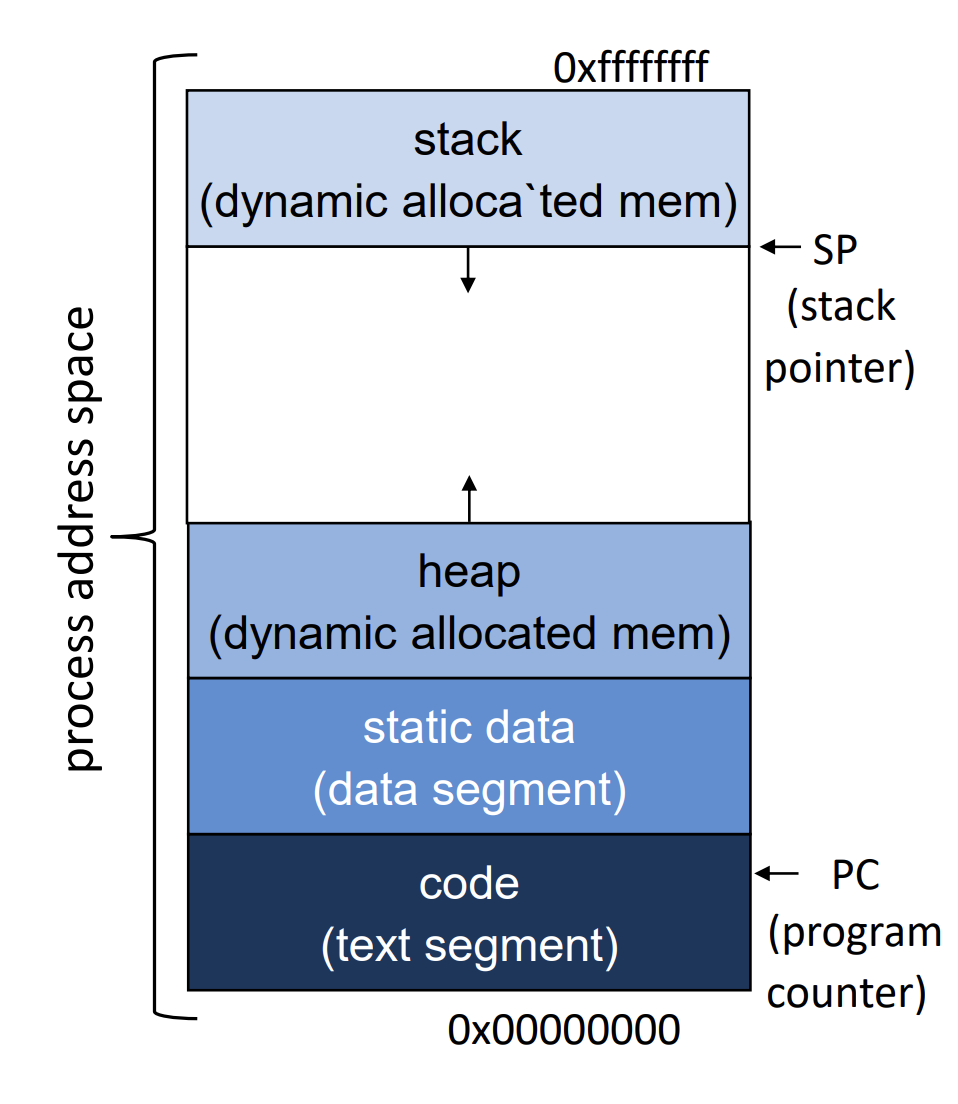
\includegraphics[width=\linewidth]{../Assets/process_memory.png}
  \end{minipage}
\end{center}



\paragraph{Process States}
A process can be in one of the following states:
\begin{itemize}
  \item \textbf{Running:} The process is currently being executed by the CPU.
  \item \textbf{Ready:} The process is ready to be executed but is waiting for the CPU to become available.
  \item \textbf{Waiting:} The process is waiting for an event to occur, such as I/O completion or a signal.
  \item \textbf{Zombie:} The process has terminated but its PCB is still in the system, waiting for the parent process to read its exit status. In this state, the process has released almost all of its resources, but \blue{the PCB is still in the system}.
\end{itemize}



\begin{figure}
  \centering
  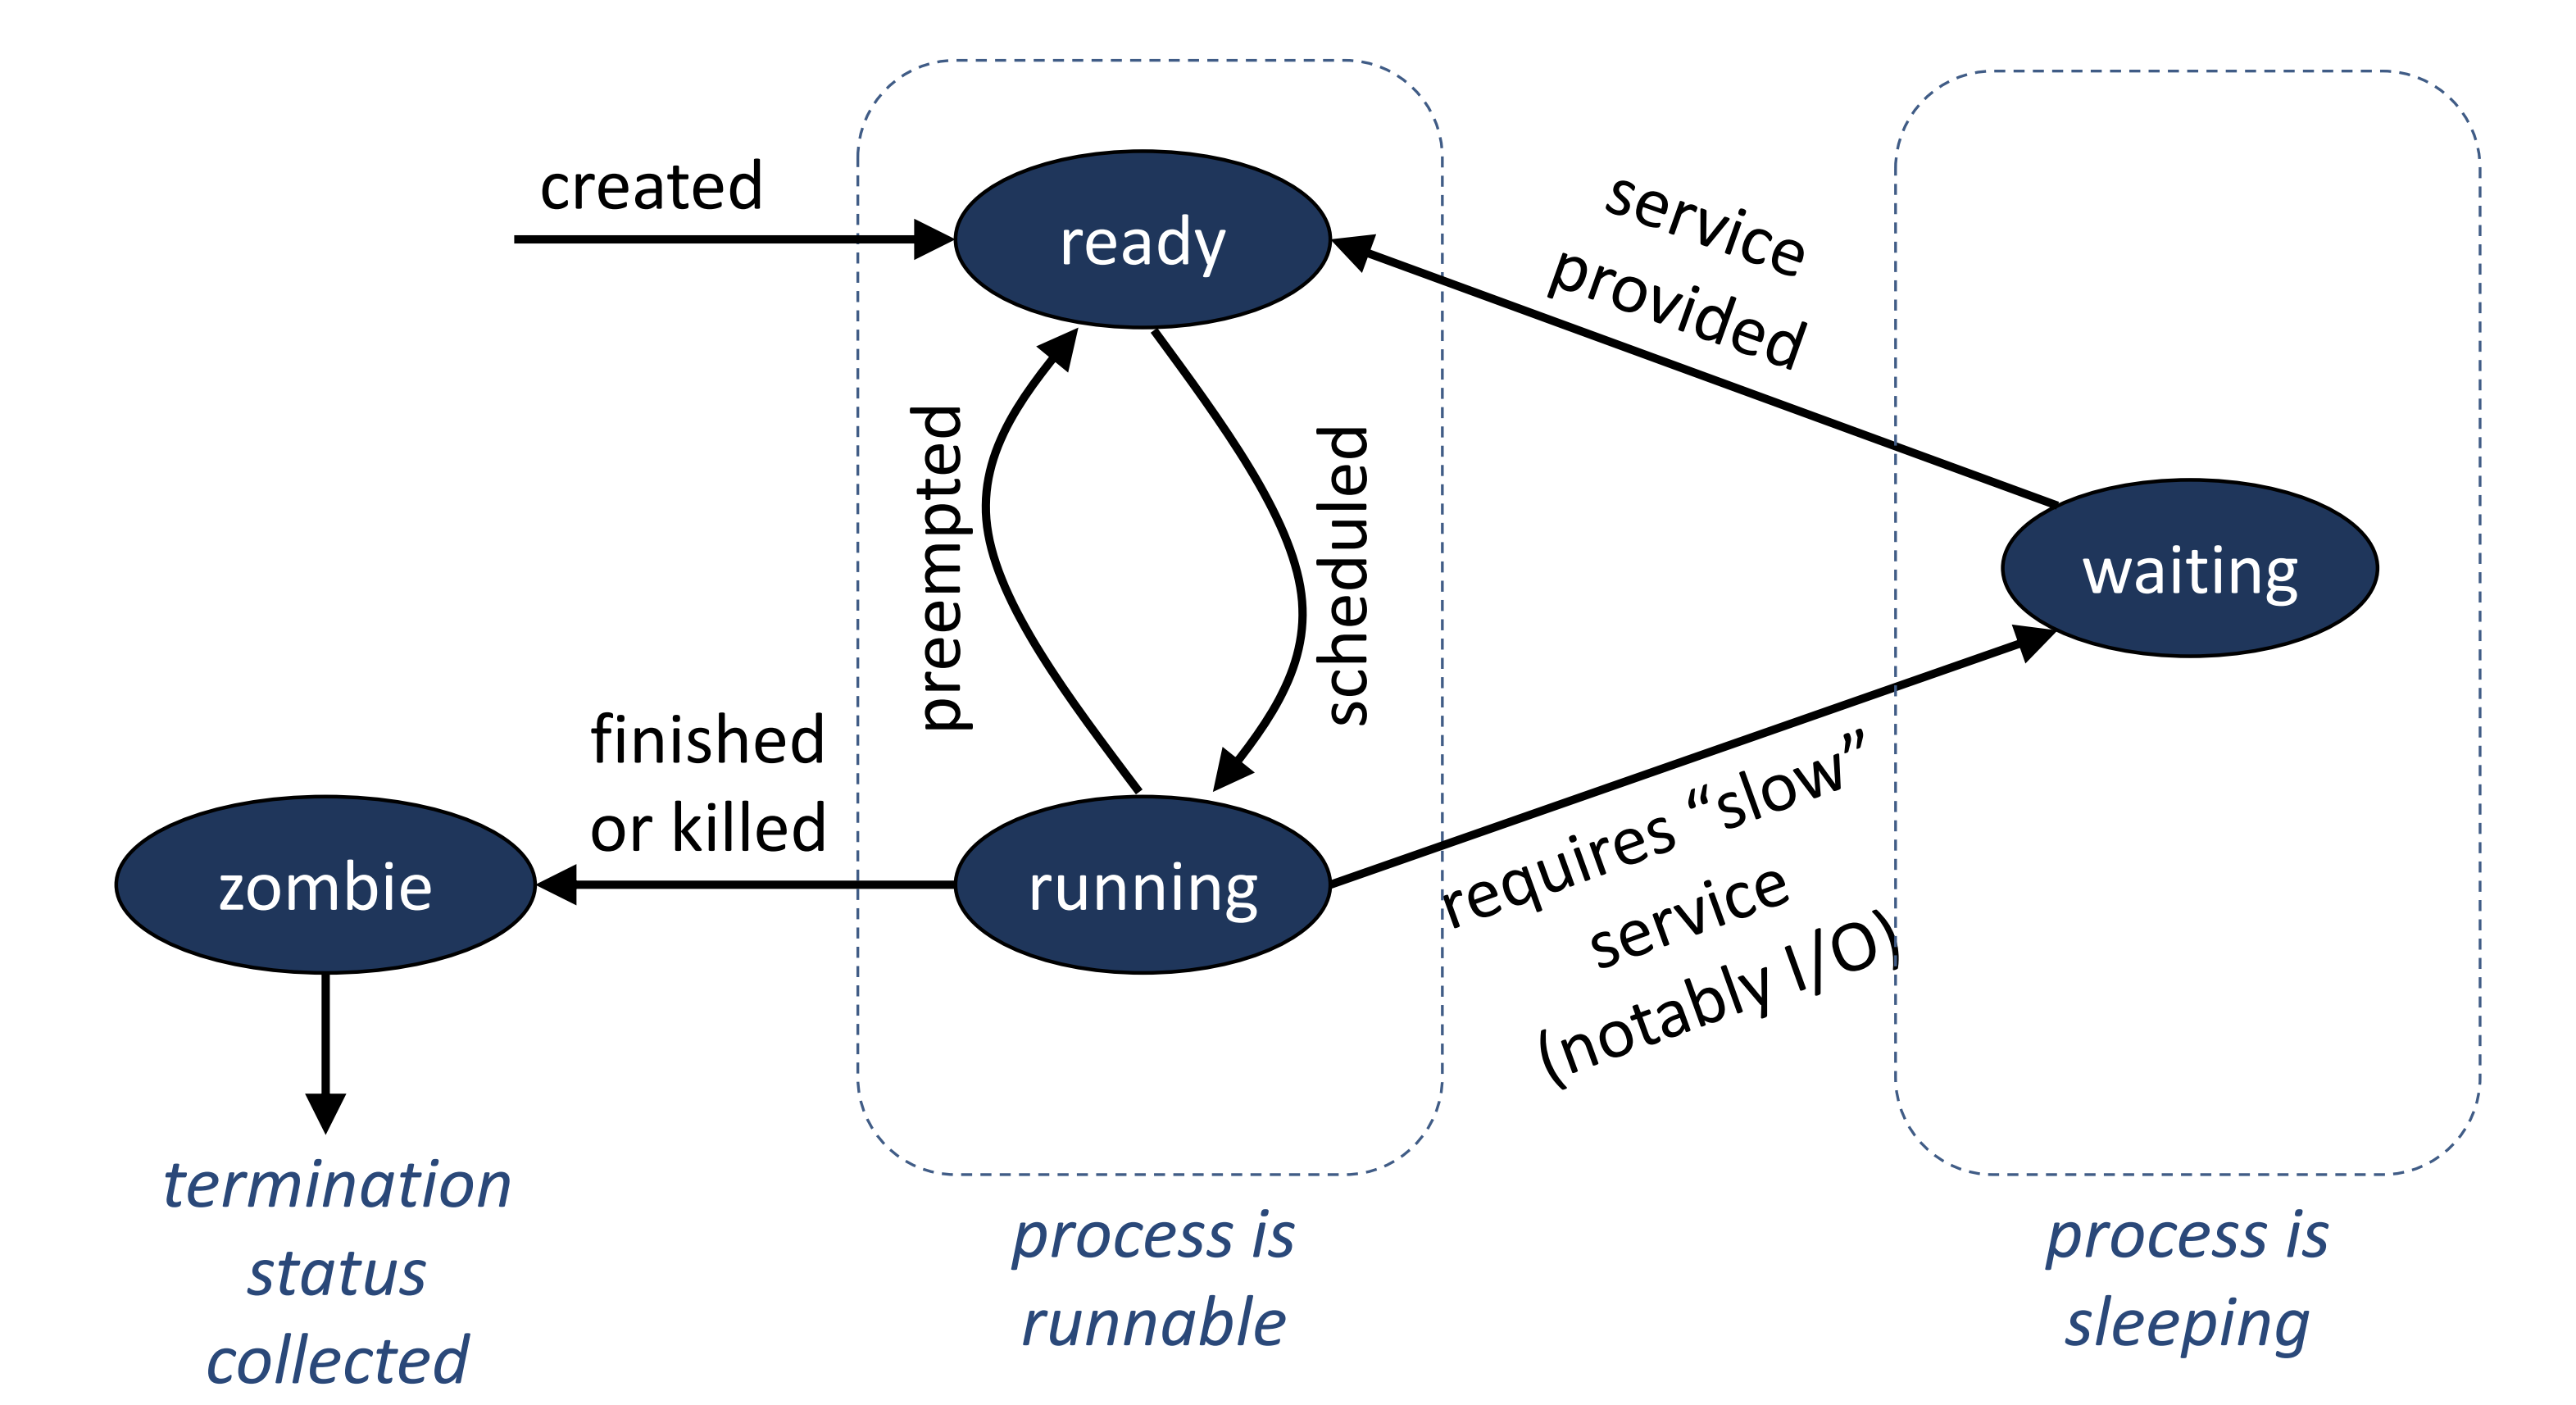
\includegraphics[width=0.8\textwidth]{../Assets/process_states.png}
  \caption{Process States}
  \label{fig:process_states}
\end{figure}


\paragraph{\code{state} Field in PCB} Each PCB keeps a \blue{32bit} \code{state} variable where each bit indicates one of the following states:
\begin{enumerate}
  \item \code{\textbf{TASK\_RUNNING :}} The task is either running or ready to run

  \item \code{\textbf{TASK\_ZOMBIE :}} The task has terminated but is still in the system

  \item \code{\textbf{TASK\_INTERRUPTIBLE :}} The task is waiting for an event to occur, but it can be interrupted by signals and come back to TASK\_RUNNING state.

  \item \code{\textbf{TASK\_UNINTERRUPTIBLE :}} The task is waiting for an event to occur, but it cannot be interrupted by signals. \gray{e.g. page fault, you can't run anything (or handle any other signals) until the page fault is handled to an end.}

  \item \code{\textbf{TASK\_STOPPED :}} The task has been stopped in a controlled manner by a \green{different} task, e.g. by a debugger or by the user pressing Ctrl+Z in the terminal.
\end{enumerate}


As we saw in "ATAM", each process can only access a certain set of utilities and functions, those who require privilege level 3 (user mode). So to access the OS services, a process must use \textbf{system calls} which are functions provided by the OS that allow processes to request services from the OS. System calls are typically implemented in the OS kernel and provide a controlled interface for processes to interact with the OS.

\vspace{1em}

Each \textit{syscall}, in case of an error, will change the \texttt{errno} variable to indicate the error type. The \texttt{errno} variable is a global variable that is set by system calls and some library functions in the event of an error to indicate what went wrong. It is defined in the header file \texttt{errno.h}. {\color{blue}\textbf{Note:} \texttt{errno} is not reset to 0 after a successful syscall, so it must be checked immediately after the syscall, and be reset before usage if need be} (if there is not any other way to make sure there is an error indeed).\\
i.e. \code{errno = <Number of Last Syscall Error>;}

\vspace{1em}

As noted above, each process must be \code{wait()}ed for by its parent process to be able to release its PCB and resources. This is done by the \texttt{wait()} syscall, which suspends the calling process until one of its children terminates. In case {\color{red} the parent process terminates before the child}, the child process {\color{red} becomes an orphan process and is adopted by the init process (PID 1)}, which will then wait for it to terminate and release its resources.


\paragraph{Process Management} The OS offers various system calls to manage processes, including: \gray{(More details in the functions reference)}
\begin{itemize}
  \item \texttt{fork()}: Creates a new process by duplicating the calling process. The new process is called the child process, and the calling process is called the parent process. For the child, the return value is \code{0}, and for the parent its the pid of the child, (on failure \(-1\) for parent).
  \item \texttt{exec()}: Replaces the current process image with a new process image, effectively running a different program in the same process.
  \item \texttt{wait()}: Suspends the calling process until one of its children terminates.
  \item \texttt{exit()}: Terminates the calling process and releases its resources.
  \item \texttt{getpid()}: Returns the process ID of the calling process.
  \item \texttt{getppid()}: Returns the process ID of the parent process.
  \item \texttt{kill()}: Sends a signal to a process, which can be used to terminate or suspend the process.
\end{itemize}

\paragraph{Parent Vs. Real Parent Process}
The real parent process is the one that created the current process using \code{fork()}, or the one that adopted it in case the real parent terminated before the child.

The parent process is the one \textit{tracing} the current process, e.g. using \code{ptrace()}. The parent process is the one that will receive signals from the current process, e.g. \texttt{SIGCHLD} when the current process terminates.

In most cases, the parent process is the real parent process, but it can be different in some cases, e.g. when a process is being traced by a debugger.



\paragraph{Daemon Processes}
A daemon process is a background process not controlled by the user.
To run a process as a daemon use \code{nohup <command> \&}.

Daemon names usually end with the letter "d", e.g. \texttt{sshd} (SSH daemon), \texttt{httpd} (HTTP daemon), etc.


\paragraph{Idle \& Init} The \code{idle} process is the first one that the system loads, with \code{pid=0}, and it utilized \code{hlt} when no process is ready to run. The next one is \code{init} which is created by idle, with \code{pid=1}, and it created all other processes. Every orphan process becomes the child of \code{init}.

\paragraph{Process List} The OS maintains a \blue{cyclic double linked list} of all processes, allowing for efficient process management and scheduling. The list starts with \code{idle} then \code{init}, where \code{idle} is the head of the list pointed to by \blue{\code{init\_task}}.


% ===================================================== Signals Section
\newpage
\section*{Signals}
\paragraph{Signals}
Signals are "notifications" sent to a process to asynchronously notify it that some event has occurred.

* Receiving a signal only occurs when returning from kernel mode, which in turn invokes the corresponding signal handler, i.e. \blue{signal handling is in user mode}.

** Default signal handling actions: Either die or ignore

*** In case of several signals from different types, they will be handled by the order of their definition in the signals register.


\vspace{1em}

Each signal has a name, a number (1-31), and a default action. All but 3 signals can be blocked, i.e. ignored until the process is ready to handle them. The 3 signals that cannot be blocked are:
\begin{itemize}
  \item \texttt{SIGKILL}: Used to forcefully terminate a process. (Process becomes a zombie)
  \item \texttt{SIGSTOP}: Used to suspend the receiving process. (Make it sleep) The signals is sent when the user presses Ctrl+Z in the terminal. {\color{gray}Note: In truth Ctrl+Z sends the \texttt{SIGTSTP} signal, however, we don't learn about the differences between the two signals in this course.}
  \item \texttt{SIGCONT}: Used to resume a suspended process, usually sent after a \texttt{SIGSTOP} signal. The handler for this signal can be customized but it {\color{red}will always} resume the process.
\end{itemize}
\texttt{SIGSTOP} and \texttt{SIGCONT} are useful for debugging purposes, allowing the user to pause and resume the execution of a process.

\paragraph{Signal Handling}
A process can define a custom signal handler for a specific signal using the \texttt{signal()} or \texttt{sigaction()} {\color{gray}preferred} system calls.
To ignore a signal, the process can set its handler to \texttt{SIG\_IGN}. To restore the default action for a signal, the process can set its handler to \texttt{SIG\_DFLT}. \blue{code{signal\_struct}} is the kernel structure in PCB that holds the signal handlers for the process.

\paragraph{Signal Masking}
A process can block signals using the \texttt{sigprocmask()} system call, which allows the process to specify a set of signals to block. This is allows the process to overcome \textit{Race Conditions} resulted from the asynchronous nature of signals.\\
\indent This is achieved by maintaining a set of currently blocked signals \& a set of masked signals which is saved in the {\color{blue}PCB}.\\
\texttt{Blocked Signals} = mask array.\\
\texttt{Pending Signals} = signals that were sent to the process while it was blocked, and will be handled when the process unblocks them.

When handling a signal, the handler masks signals of the same type (of the one being handled), to prevent problems of reentrancy.

\paragraph{Common Signals} the following are some of the most common signals:
\begin{enumerate}
  \item \textbf{\code{SIGSEGV, SIGBUS, SIGILL, SIGFPE}}: These are driven by the associated \blue{(HW) interrupts} - The OS gets the associated interrupt, then the OS interrupt handler sees to it that the misbehaving process gets the associated signal, lastly the signal handler is invoked.
        \begin{itemize}
          \item \texttt{SIGSEGV}: Segmentation violation (illegal memory reference, e.g., outside an array).
          \item \texttt{SIGBUS}: Dereference invalid address (null/misaligned, assume it's like SEGV).
          \item \texttt{SIGILL}: Illegal instruction (trying to invoke privileged instruction).
          \item \texttt{SIGFPE}: Floating-point exception (despite the name, \textit{all} arithmetic errors, not just floating point. e.g., division by zero).
        \end{itemize}

  \item \textbf{\code{SIGCHLD}}: Parent \gray(and then real parent) get it whenever \code{fork()}ed child terminates or is \code{SIGSTOP}-ed.

  \item \textbf{\code{SIGALRM}}: Get a signal after some specified time, can be set using the \blue{\code{alarm()} \& \code{setitimer()}} system calls.

  \item \textbf{\code{SIGTRAP}}: When debugging/single-stepping a process, the debugger can set a breakpoint in the code, which will cause the process to receive a \texttt{SIGTRAP} signal when it reaches that point.

  \item \textbf{\code{SIGUSR1, SIGUSR2}}: User-defined signals, user can decide the meaning of these signals and their handlers.

  \item \textbf{\code{SIGPIPE}}: Write to pipe with no readers.

  \item \textbf{\code{SIGINT}}: Sent when the user presses Ctrl+C in the terminal. The default action is to terminate the process, but it can be customized.

  \item \textbf{\code{SIGXCPU}}: Delivered when a process used up more CPU than its soft-limit allows: soft/hard limits are set using the \blue{\code{setrlimit()}} system call. Soft-limits warn the process its about to exceed the hard-limit, Exceeding the hard-limit will cause \code{SIGKILL} to be sent to the process.

  \item \textbf{\code{SIGIO}}: Can configure file descriptors such that a signal will be delivered whenever some I/O is ready.

        Typically makes sense when also configuring the file descriptor to be \textit{non-blocking}, e.g., when \code{read()}ing from a non-blocking file descriptor, the system call immediately returns to user if there's currently nothing to read. In this case, \code{errno} will be set to \code{EAGAIN=EWOULDBLOCK}.


  \item \textbf{Signal 0:} The null signal, which is used to test for the existence of a process.
\end{enumerate}


\begin{samepage}
  \begin{center}
    \textbf{Signals Vs. Interrupts}
    \rowcolors{2}{gray!15}{white}
    \begin{tabular}{|>{\raggedright\arraybackslash}p{4.5cm}|>{\raggedright\arraybackslash}p{5.5cm}|>{\raggedright\arraybackslash}p{5.5cm}|}
      \hline
      \rowcolor{blue!30}
       & \textbf{interrupts}                                                                      & \textbf{signals} \\
      \hline
      Who triggers them? \newline Who defines their meaning?
       & Hardware: \newline CPU cores (sync) \& other devices (async)
       & Software (OS), \newline HW is unaware                                                                       \\
      \hline
      Who handles them? \newline Who (un)blocks them?
       & OS
       & processes                                                                                                   \\
      \hline
      When do they occur?
       & Both synchronously \& asynchronously
       & Likewise, but, technically, \newline invoked when returning \newline from kernel to user                    \\
      \hline
    \end{tabular}
  \end{center}
\end{samepage}





% =====================================================
% ================== Lecture 3 ========================
% =====================================================


\Topic{IPC - Inter-Process Communication}

\section*{Threads \& IPC}


\paragraph{Multiprocessing}
Using several CPU cores (=processors) for running a single job to solve a single "problem".


\begin{center}
  \begin{minipage}{0.45\textwidth}
    \vspace{0pt} % force top alignment
    \centering
    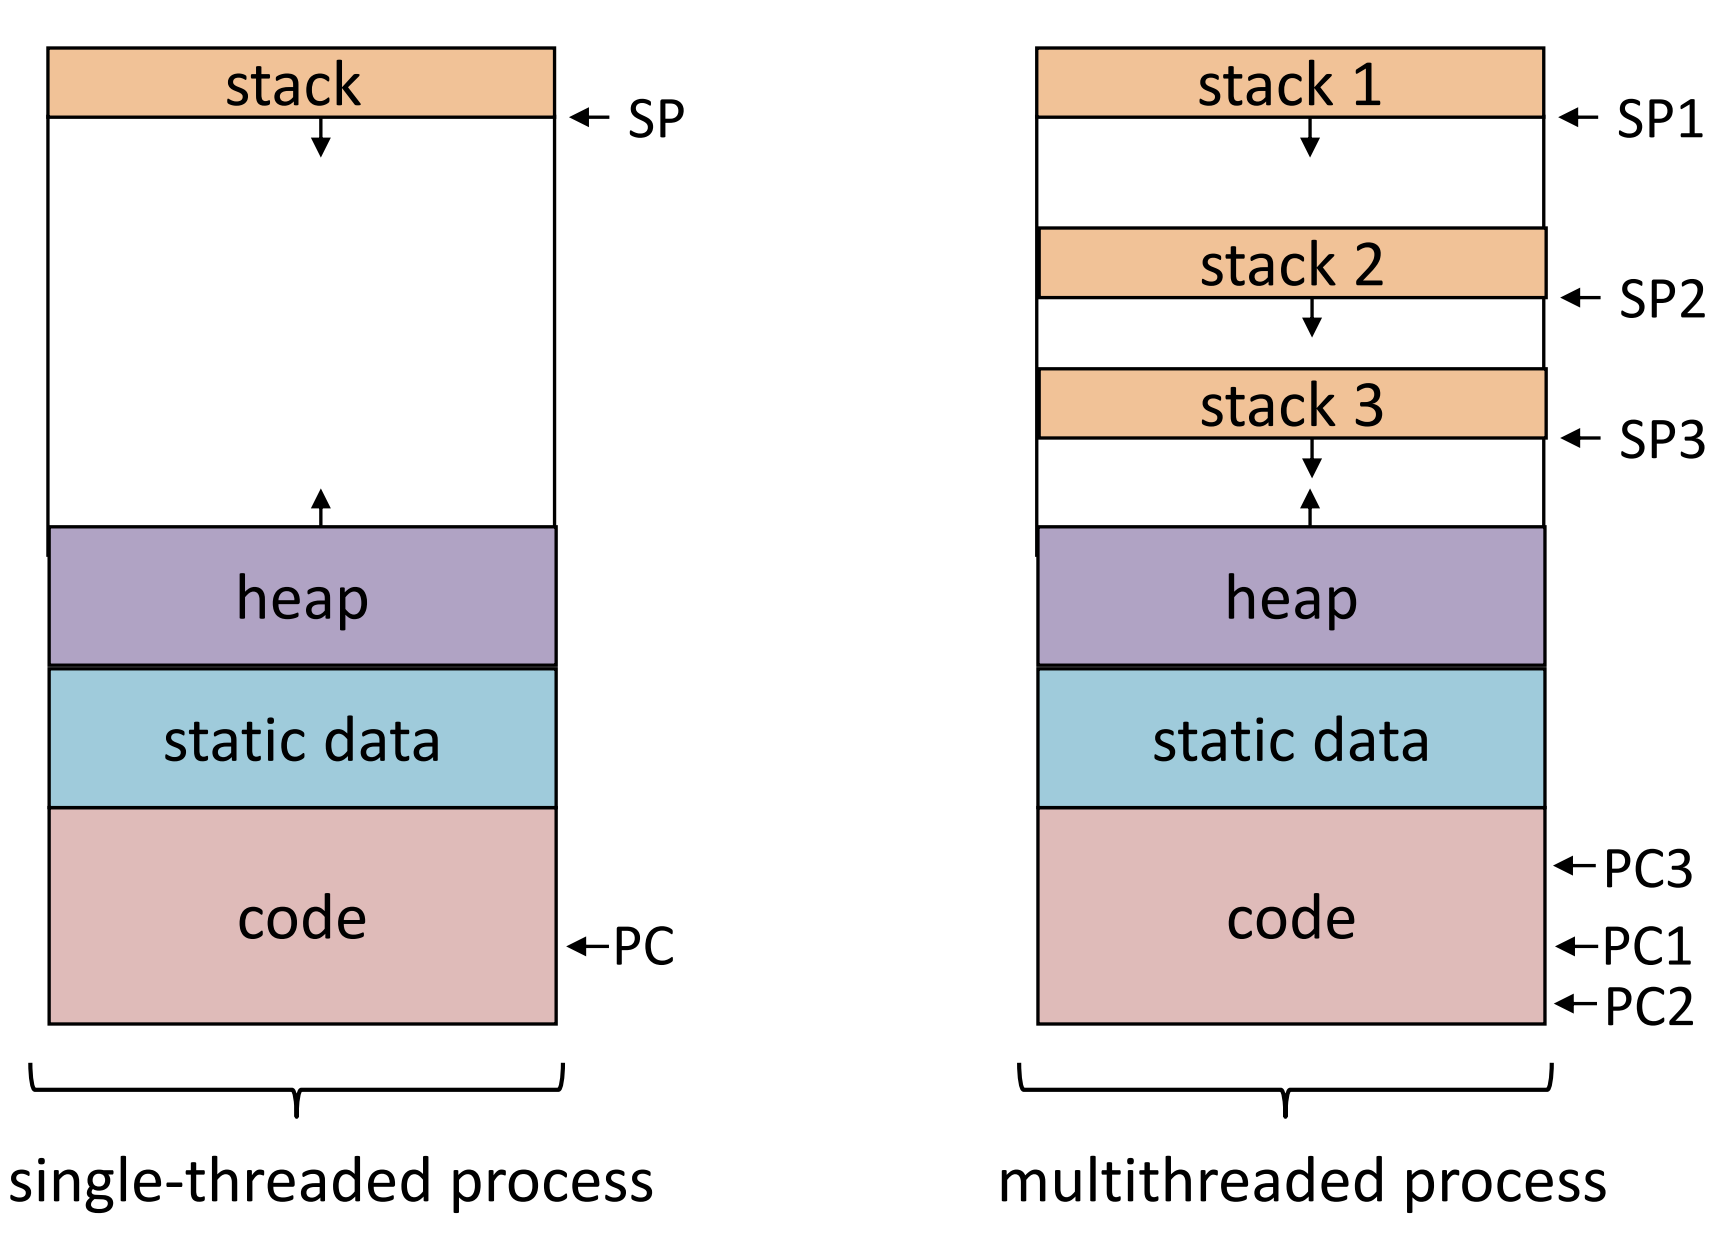
\includegraphics[width=\linewidth]{../Assets/thread_stack.png}
  \end{minipage}\hfill
  \begin{minipage}{0.5\textwidth}
    \vspace{0pt} % force top alignment  
    \paragraph{Threads}
    A process can have multiple threads, which share (nearly) everything, including the process's memory space, file descriptors, heap, static data, code segment and more.

    \hspace*{2em}However, each thread has its own stack, registers, and program counter. But they can still access each other's stack since they share the same memory space.
  \end{minipage}
\end{center}

Note that \blue{\textit{Global/Static Variables \& Dynamically Allocated Memory}} are shared between threads since they are stored in the Static Data Segment and the Heap, respectively, which are shared between all threads of a process. However, \red{\textit{Local Variables}} are not shared between threads since they are stored in the stack, which is unique to each thread.


\begin{samepage}
  \begin{center}
    \rowcolors{2}{gray!15}{white}
    \begin{tabular}{|>{\raggedright\arraybackslash}p{6cm}|
      >{\centering\arraybackslash}p{4cm}|
      >{\centering\arraybackslash}p{4cm}|}
      \hline
      \rowcolor{blue!30}
                                       & \textbf{Unique to Process} & \textbf{Unique to pthread} \\
      \hline
      Registers (notably PC)           & Y                          & Y                          \\
      Execution stack                  & Y                          & Y                          \\
      Memory address space             & Y                          & \red{N}                    \\
      Open files                       & Y                          & \red{N}                    \\
      Per-open-file position (=offset) & Y                          & \red{N}                    \\
      Working directory                & Y                          & \red{N}                    \\
      User/group credentials           & Y                          & \red{N}                    \\
      Signal handling                  & Y                          & \red{N}                    \\
      \hline
    \end{tabular}
  \end{center}
\end{samepage}


\newpage
\paragraph{OpenMP} Open Multi-Processing (OpenMP) consists of a set of compiler \textit{'pragma'} directives that allows the compiler to generate multi-threaded code for parallel execution.

\begin{center}
  \begin{minipage}{0.9\textwidth}
    \begin{lstlisting}
    #pragma omp parallel for
    for (i = 0; i < N; i++) {
            arr[i] = 2*i;
    } \end{lstlisting}
  \end{minipage}
\end{center}


\paragraph{Pthreads} POSIX threads (pthreads) is a standard for multi-threading in C/C++. It provides a set of functions to create and manage threads, as well as to synchronize them. 




\noindent % Prevents indentation before the first minipage
% --- BEGIN LEFT COLUMN (TEXT) ---
\begin{minipage}[t]{0.48\textwidth}
\begin{center}
  \textbf{Common Functions}
\end{center}
The following are some of the most commonly used pthread functions:
\begin{itemize}
    \item \textbf{\code{pthread\_create(...)}}: Creates a new thread that starts executing a given function. The thread ID is stored in a pointer.
    
    \item \textbf{\code{pthread\_self()}}: Returns the thread ID of the calling thread. This ID is internal to the pthread library.

    \item \textbf{\code{pthread\_exit(...)}}: Terminates the calling thread and makes its exit status available to any thread that joins it.

    \item \textbf{\code{pthread\_cancel(...)}}: Sends a request to terminate a specified thread. The thread's exit status is set to \code{PTHREAD\_CANCELED}.

    \item \textbf{\code{pthread\_join(...)}}: Blocks the calling thread until a specified thread terminates, then retrieves its exit status and frees its resources.
\end{itemize}
\end{minipage}
\hfill % This creates a flexible space between the two columns
% --- BEGIN RIGHT COLUMN (TABLE) ---
\begin{minipage}[t]{0.5\textwidth}
  \begin{center}
    \textbf{Thread Termination}
  \end{center}
\centering % Centers the table within the minipage
\rowcolors{2}{gray!15}{white}
% Note: Column widths have been adjusted to fit inside the minipage
\begin{tabular}{|>{\raggedright\arraybackslash}p{0.45\linewidth}|
    >{\centering\arraybackslash}p{0.2\linewidth}|
    >{\centering\arraybackslash}p{0.25\linewidth}|}
    \hline
    \rowcolor{blue!30}
    \textbf{Reason for Termination} & \textbf{Thread Terminates?} & \textbf{Process Terminates?} \\
    \hline
    Calling \code{pthread\_exit()} & Yes & Not necessarily \\
    Calling \code{pthread\_cancel()} & Yes & Not necessarily \\
    Return from \code{start\_routine} & Yes & Not necessarily \\
    \hline
    Calling \code{exit()} & Yes & Yes \\
    Illegal operation & Yes & Yes \\
    Return from \code{main} & Yes & Yes \\
    \hline
\end{tabular}
\end{minipage}

\paragraph{Threads in Linux} In Linux, threads are implemented as *processes* with a shared memory space. Each thread has its own PCB, but they share the same memory address space, file descriptors, and other resources. Threads do not have family ties between one another.

\paragraph{Thread Groups} A thread group is a collection of threads that share the same process ID (PID) and are managed by the same process. In Linux, each thread group has a unique group ID (TGID), which is the PID of the first thread in the group. The TGID is used to manage signals and other resources shared by the threads in the group.

Since each thread has his own PCB and PID, to send a signal to all threads in a thread group, the signal must be sent to the TGID (the PID of the first thread in the group). Each PCB contains a field \code{thread\_group} which points to the head of the linked list of all threads in the group. 

The syscall \code{getpid()} returns the \code{TGID} of the calling thread. The personal "PID" of each thread is called \code{TID} (Thread ID), which is the same as the personal "PID" of the thread's PCB. The syscall \code{gettid()} returns the TID of the calling thread.


\paragraph{\code{clone()}} The syscall:
\code{clone(int (*fn)(void *), void *child\_stack, int flags, void *arg);}  
is used to create a child process that shares resources with the parent process. The parameters are:
\begin{itemize}
  \item \code{fn}: A pointer to the function that will be the main function of the child process.
  \item \code{child\_stack}: A pointer to the \gray{user} stack that will be used by the child process. \gray{The highest address of the stack is passed, i.e. the top of the stack.}
  \item \code{arg}: A pointer to the argument that will be passed to the function \code{fn}.
  \item \code{flags}: A bitmask that specifies which resources will be shared between the parent and child processes. The flags can include:
  \begin{itemize}
    \item \code{CLONE\_VM}: Share the same memory address space.
    \item \code{CLONE\_FS}: Share the same filesystem information (e.g., current working directory).
    \item \code{CLONE\_FILES}: Share the same file descriptor table.
    \item \code{CLONE\_PARENT}: Share the same parent process as the parent of the calling thread.
    \item \code{CLONE\_THREAD}: Create a new thread in the same thread group.
  \end{itemize}
\end{itemize}
The return value is the TID of the child.






\paragraph{File Descriptors} A non-negative integer representing an I/O "channel" on some device. File descriptors are saved in the process's \code{PCB} inside the \code{FDT} (File Descriptor Table), which is an array of pointers to \textit{file objects}, each representing an open file or device. So in fact, an FD is an index to a kernel array of channels.

Processes \red{don't} share \code{PCB} nor \code{FDT} but they \blue{can share file descriptors}, i.e. two processes can have the same file descriptor pointing to the same file object, which allows them to share the same open file or device. Upon forking, the child process inherits a copy of the parent's \code{FDT}. \blue{Note:} Threads \blue{do} share the same \code{FDT}.



\paragraph{Pipes} A pipe is a unidirectional communication channel between two processes, allowing one process to send data to another. Pipes are a pair of two file descriptors \code{int pipe\_fd[2]}. Each integer is a handle to a kernel communication object ("file"), \ul{pipes reside }\red{\ul{only}}\ul{ on DRAM (memory) and never on the disk, and they are not in the filesystem}. \gray{(pipes are anonymous shared pages)}
\begin{itemize}
  \item \code{pipe\_fd[0]} = read side of the communication channel.
  \item \code{pipe\_fd[1]} = write side of the communication channel.
  \item Everything written via \code{pipe\_fd[1]} can be read via \code{pipe\_fd[0]}.
  \item \red{Blocking}: If the read side is empty, the read operation will block until data is written to the write side. If the write side doesn't have enough space for \ul{all} the data, the write operation will block until space is available.
  \item \red{EOF}: If the write side is closed and the pipe is empty, the read operation will return 0, indicating EOF (End of File). 
  \item \red{\code{SIGPIPE}}: Writing to a pipe whose read end is \code{close()}d will result in a \code{SIGPIPE} signal.
\end{itemize}

\paragraph{FIFO (Named Pipe)} A FIFO is a named pipe that allows for communication between unrelated processes (no family connection), i.e. it's a public "file". FIFO is a file even though \ul{it is NOT on the disk}, though it can be swapped there. 

To make a FIFO, use the \code{mkfifo(const char *pathname, mode\_t mode)} system call, which creates a special file in the filesystem with path \code{pathname} and permissions \code{mode}. The FIFO can then be opened by any process using the \code{open()} system call, just like a regular file. The FIFO is bidirectional, thus having one FD. 

A process that opens FIFO for read only, will block until another process opens it for write, and vice versa. If one opens it as both read \& write (O\_RDWR) then it will \red{not} be blocking. *The read write rules are similar to the one of pipe.

FIFOs are \red{not} removed from the system automtically (unlike pipes whom do), so they have to be \textit{explicitly} removed by \code{rm}\code{unlink} for example. Meaning a closed FIFO can be reopened until removed completely.

\begin{samepage}
  \begin{center}
    \rowcolors{2}{gray!15}{white}
    \begin{tabular}{|>{\raggedright\arraybackslash}p{4cm}|
      >{\raggedright\arraybackslash}p{6cm}|
      >{\raggedright\arraybackslash}p{5cm}|}
      \hline
      \rowcolor{blue!30}
      \textbf{Multi-tasking} & \textbf{Multi-programming} & \textbf{Multi-processing} \\
      \hline
      Having multiple processes \textit{time slice} on the same CPU core.
                             &
      Having \textit{multiple jobs} in the system (either on the same core or on different cores). \gray{i.e. the existence of multiple processes in the system, regardless of whether they are running on the same core or not.}
                             &
      Using \textit{multiple processors (CPU cores) for the same job} in parallel. \gray{i.e. creating multiple threads to run on different cores for the same process.}
      \\
      \hline
    \end{tabular}
  \end{center}
\end{samepage}





\newpage
\section*{Intro. Context Switching \& Caching}
\paragraph{Context Switching} is the process of saving the state of a currently running process and restoring the state of another process to allow it to run. This is done by the OS kernel and is necessary for multitasking, allowing multiple processes to share the CPU.
\begin{itemize}
  \item \textbf{Context} = the state of a process, including its registers, program counter, stack pointer, and memory management information.
  \item \textbf{Context Switch} = the process of saving the context of the currently running process and restoring the context of another process.
\end{itemize}

\paragraph{Context Switch Overhead} consists of two components:
\begin{itemize}
  \item \textbf{Direct Overhead:} The measurable time it takes to perform the context switch, which includes saving the current process's state and restoring the next process's state.
  \item \textbf{Indirect Overhead:} The time it takes for the CPU to cache the new process's data, which can be significant if the new process's data is not already in the CPU cache.
\end{itemize}

\paragraph{Cashing} The CPU cache is a small, fast memory that stores frequently accessed data to speed up access times. The Cache allows the CPU access to a fast memory that is closer to the CPU than the main memory (DRAM), and a larger one than the CPU registers. The cache works because of the \blue{\textit{Principle of Locality}}:
\begin{itemize}
  \item \textbf{Temporal Locality:} If at one point in time a particular memory location is referenced, then it is likely that the same location will be referenced again soon.
  \item \textbf{Spatial Locality:} If a particular memory location is referenced at a particular time, then it is likely that nearby memory locations will be referenced soon.
\end{itemize}



\paragraph{Copy-on-Write (COW)} The \code{fork()} system call creates a copy of the address space of the parent, but:
\begin{itemize}
  \item It only creates a \textit{logical} copy.
  \item There is no physical duplication of the memory pages, until we really need to write to them (from either process). And even then, only the page that is being written to is duplicated. \gray{(More details in the virutal memory lectures)}
\end{itemize}


\paragraph{User Level Threads (ULTs)} are threads that are managed by the user-level library, rather than the OS kernel. ULTs are not visible to the OS, which means that the OS does not know about them and does not schedule them. This allows for faster context switching between ULTs, but it also means that the OS cannot take advantage of multiple CPU cores to run ULTs in parallel.

The usage of ULTs is mainly for concurrent programming, where we want multiple multiple tasks to progress in parallel without the overhead of kernel-level threads.





% =====================================================
% =============== BOOT AND MODULES ====================
% =====================================================


\newpage
\Topic{Boot \& Modules}

\section*{Booting the OS}

\paragraph{Operating System at Power ON} When powering on a PC, the OS has yet to load into the memory, as it resides on the disk. So we need to load the OS from the disk to the memory, but we need the OS to do that! So the solution is hierarchal booting: 
\begin{enumerate}
  \item The \blue{BIOS} code is loaded into the memory (DRAM) and the CPU starts executing it.

  \item The BIOS loads \blue{the first sector of the disk (MBR)} to the memory

  \item The MBR code loads the \blue{boat loader}

  \item The boot loader loads the \blue{kernel} of Linux

  \item The kernel loads the init process (\code{/init}) and runs it
\end{enumerate}


\paragraph{BIOS (Basic Input/Output System)} The BIOS is located in the motherboard, loaded to the same memory location always, and is the first code that runs when the computer is powered on. It performs the following tasks:
\begin{itemize}
  \item Identify the hardware components of the system that are connected.
  \item Check if basic hardware components are working properly (screen, keyboard, etc)
  \item Search for the device (from a pre-defined list) that enables booting (bootable device)
  \item If the device is not found, the BIOS shows an error message and stops the booting process. Otherwise, it loads the \ul{first sector} of the device to a constant place in memory.
\end{itemize}


\paragraph{MBR (Master Boot Record)} The bootable device holds in the first sector (512 bytes), the MBR, which is a very basic assembly program that is used to load the boot loader, since it requires more space than the MBR can provide. 

\paragraph{Boot Loader (Grub)} GRUB (GRand Unified Bootloader) is a boot loader package from the GNU Project. It allows users to choose between multiple operating systems at boot time and can load a variety of operating systems, including Linux, Windows, and others. 


\paragraph{Loading the Kernel} The boot loader loads the kernel in the following steps:
\begin{enumerate}
  \item Load the compressed kernel image from the disk to the memory.
  \item Load a basic initial filesystem (initramfs or initrd)
  \begin{itemize}
    \item The initial filesystem includes the necessary modules for the linux kernel to find and load the real filesystem.
  \end{itemize}
  \item The kernel runs the script \code{/init} (typically a shell script) from the initial filesystem.
  \item The \code{/init} script loads the necessary drivers and mounts the real filesystem instead of the initial one.
  \item After the real filesystem is mounted, the linux kernel runs the \code{/sbin/init} program.
\end{enumerate}


\section*{Modules}

\paragraph{Kernel Modules} are pieces of code that can be loaded into the kernel at \red{runtime}, without need to recompile the kernel. New modules can be loaded only in kernel mode (CPL=0). The primary use for modules is to implement drivers for hardware devices, but they can also be used to implement new system calls, filesystems, and other kernel features. Beware Modules run in kernel mode so they have access to everything.

The advantages of using kernel modules are: (1) Allowing to add functionality without rebooting, (2) Allowing for faster compile time of the kernel, (3) The kernel will use less space, (4) Allowing to add support for new hardware.


To implement a module we use (Beware to use kernel functions and not user functions, e.g. "kprintf" instead of "printf"):
\begin{itemize}
  \item \code{int init\_module(void)}: The function that is called when the module is loaded into the kernel. 

  \item \code{void cleanup\_module(void)}: The function that is called when the module is unloaded from the kernel.

  \item \code{module\_param(name, type, perm)}: A macro to declare a module parameter. each parameter must have a default value.
\end{itemize}



\paragraph{Devices \& Drivers} Devices are represented by special files in the filesystem, which are called \textbf{device files}, which are located in \code{/dev}. To communicate with a device, we use the standard file operations (open, read, write, close) on the device file. The kernel uses \textbf{device drivers} to handle the communication with the device. Device drivers are kernel modules that implement the necessary functions to communicate with the device.

\paragraph{Block vs Character Devices} Character devices are ones that can be accessed as a stream of bytes (e.g. keyboard, mouse, etc.), typically for transferring data and in a sequential matter. Block devices are ones that can be accessed only in multiples of blocks (e.g. hard drives), typically for storing data in random-access data.

\paragraph{Character Devices} Each character device is represented by a \textbf{major number (1-512)} and a \textbf{minor number (0-255)}. The major number identifies the driver associated with the device, while the minor number identifies the specific device. Each major number can have multiple minor numbers, and vice versa. Both numbers are found in the \code{inode} of the device file.

\vspace*{1em}
Registering a new device is done by: (default permissions are write for owner, read for others)
\begin{center}
  \textbf{\code{mknod}} \code{<Name> <Type (c for character, b for block)> <Major Number> <Minor Number>}
\end{center}


\paragraph{Pseudo-Devices} Linux provides pseudo-character devices that are not connected to any physical hardware. All of these devices share a \blue{major number of 1}.

{
\centering
\renewcommand{\arraystretch}{2.2} % Increase row height for readability
\begin{tabular}{|p{5.5cm}|p{5.5cm}|l|}
\hline
\textbf{write()} & \textbf{read()} & \textbf{device file} \\
\hline

\multirow{2}{5.5cm}{Succeeds and does nothing (data is discarded).} 
& Immediately returns EOF (end of file). 
& \texttt{/dev/null} \\
\cline{2-3}

& \multirow{2}{5.5cm}{Returns a sequence of null bytes (\texttt{\char`\\0}) of the requested length.} 
& \texttt{/dev/zero} \\
\cline{1-1}\cline{3-3}

Immediately returns ENOSPC (no space left on device). 
& 
& \texttt{/dev/full} \\
\hline

Contributes to the kernel's entropy pool from "noise".
& Returns a stream of random bytes generated at runtime.
& \begin{tabular}{@{}l@{}}
    \texttt{/dev/random}\\ 
    \texttt{/dev/urandom}\\ 
    \texttt{/dev/arandom}
  \end{tabular} \\
\hline

\end{tabular}
}





\begin{figure}[H]
  \centering
  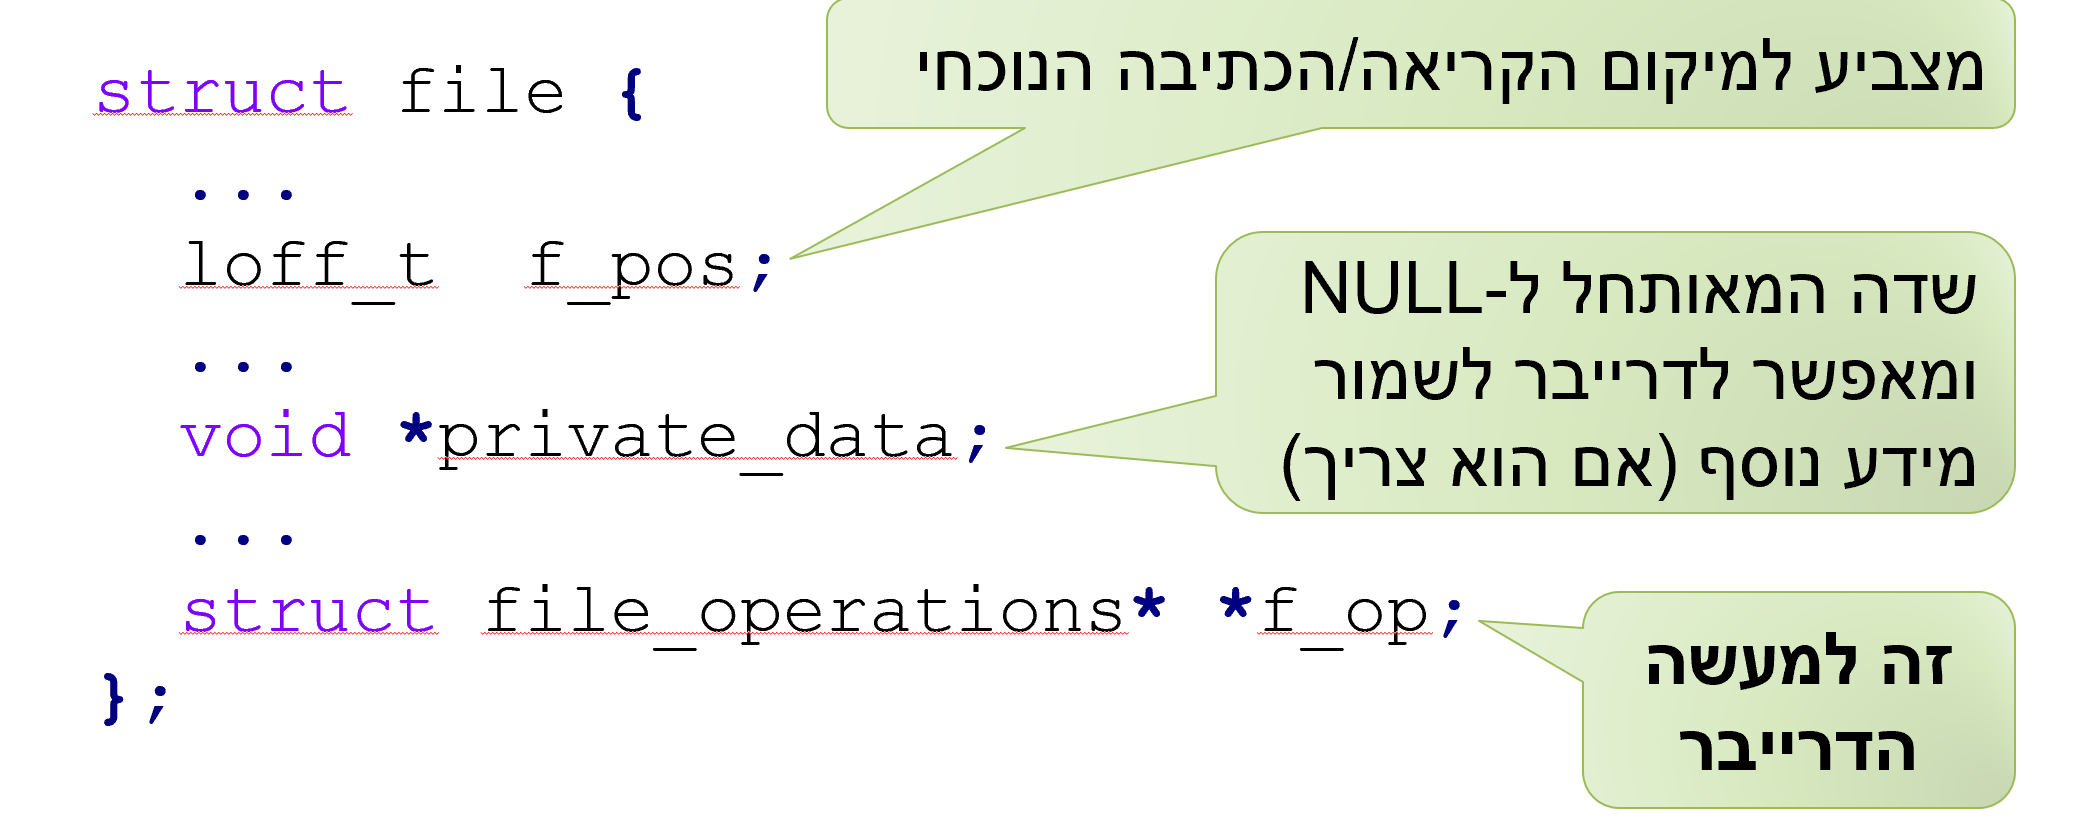
\includegraphics[width=0.8\textwidth]{fileOperations.png}
  \caption{File struct and file operations}
  \label{fig:fileOperations}
\end{figure}


\paragraph{file operations} Each file struct has a \texttt{file\_ops} field, which is a pointer to a struct that contains pointers to functions that implement the file operations for that file. These functions include:
\begin{itemize}
  \item \code{int (*open) (struct inode *, struct file *)}: Called when the file is opened. If open is null, it will succeed.  

  \item \code{int (*release) (struct inode *, struct file *)}: Called when the \ul{last} instance of the file is closed. If release is null, it will succeed.

  \item \code{int (*flush) (struct file *)}: Called when the file is closed (every time an FD is closed, not just the last one). If flush is null, it will succeed.

  \item \code{ssize\_t (*read) (struct file *, char *, size\_t, loff\_t *)}: Called when the file is read. If read is null, it will return (-EINVAL).
  
  \item \code{ssize\_t (*write) (struct file *, const char *, size\_t, loff\_t *)}: Called when the file is written to. If write is null, it will return (-EINVAL).
  
  \item \code{loff\_t (*llseek) (struct file *, loff\_t, int)}: Called when the file's offset is to be changed.
  
  \item \code{int (*ioctl) (struct inode *, struct file *, unsigned int \textbf{cmd\_id}, unsigned long \textbf{arg})}: Allows adding additional functionality to the device. Arg is an optional parameter.
\end{itemize}





\paragraph{Drivers as Modules} Drivers can be implemented as kernel modules, where \code{init\_module()} will register the driver using \code{register\_chrdev()}. Note that registering a driver only connects it with a major number, and not to a device. Unregistering a driver is done through \code{cleanup\_module()} that uses \code{unregister\_chardev()}.


\begin{figure}[H]
  \centering
  \begin{subfigure}[b]{0.48\textwidth}
    \centering
    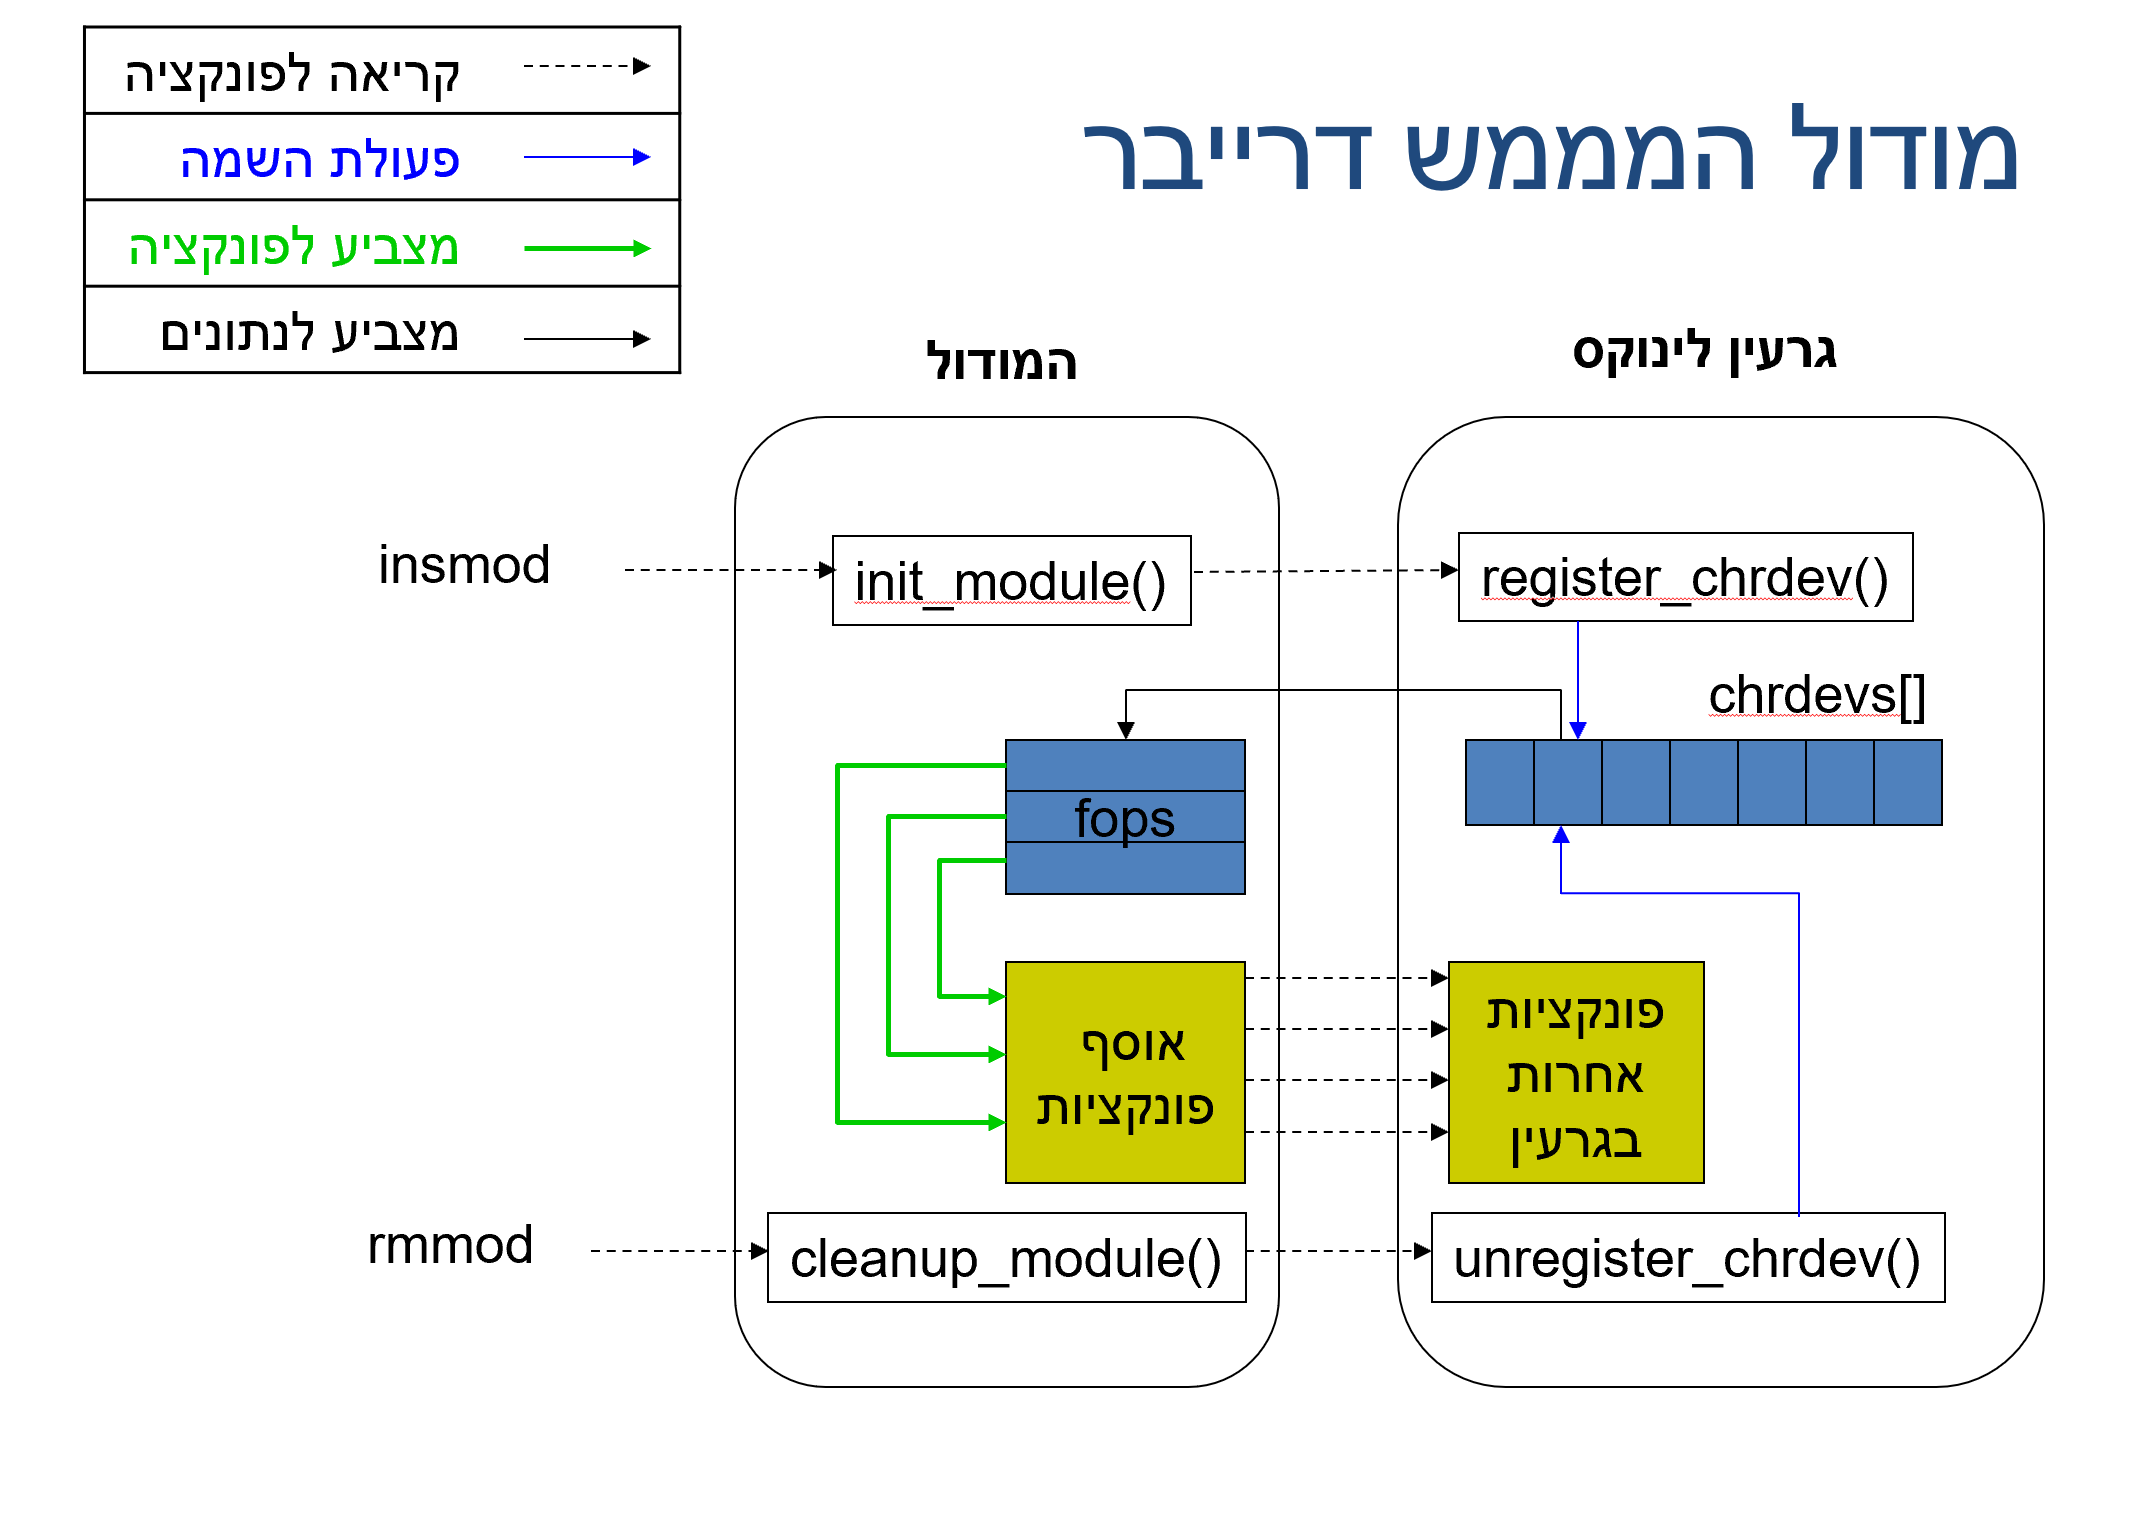
\includegraphics[width=\textwidth]{module_driver.png}
    \caption{Driver Module Flow}
    \label{fig:driver_module_flow}
  \end{subfigure}
  \hfill
  \begin{subfigure}[b]{0.48\textwidth}
    \centering
    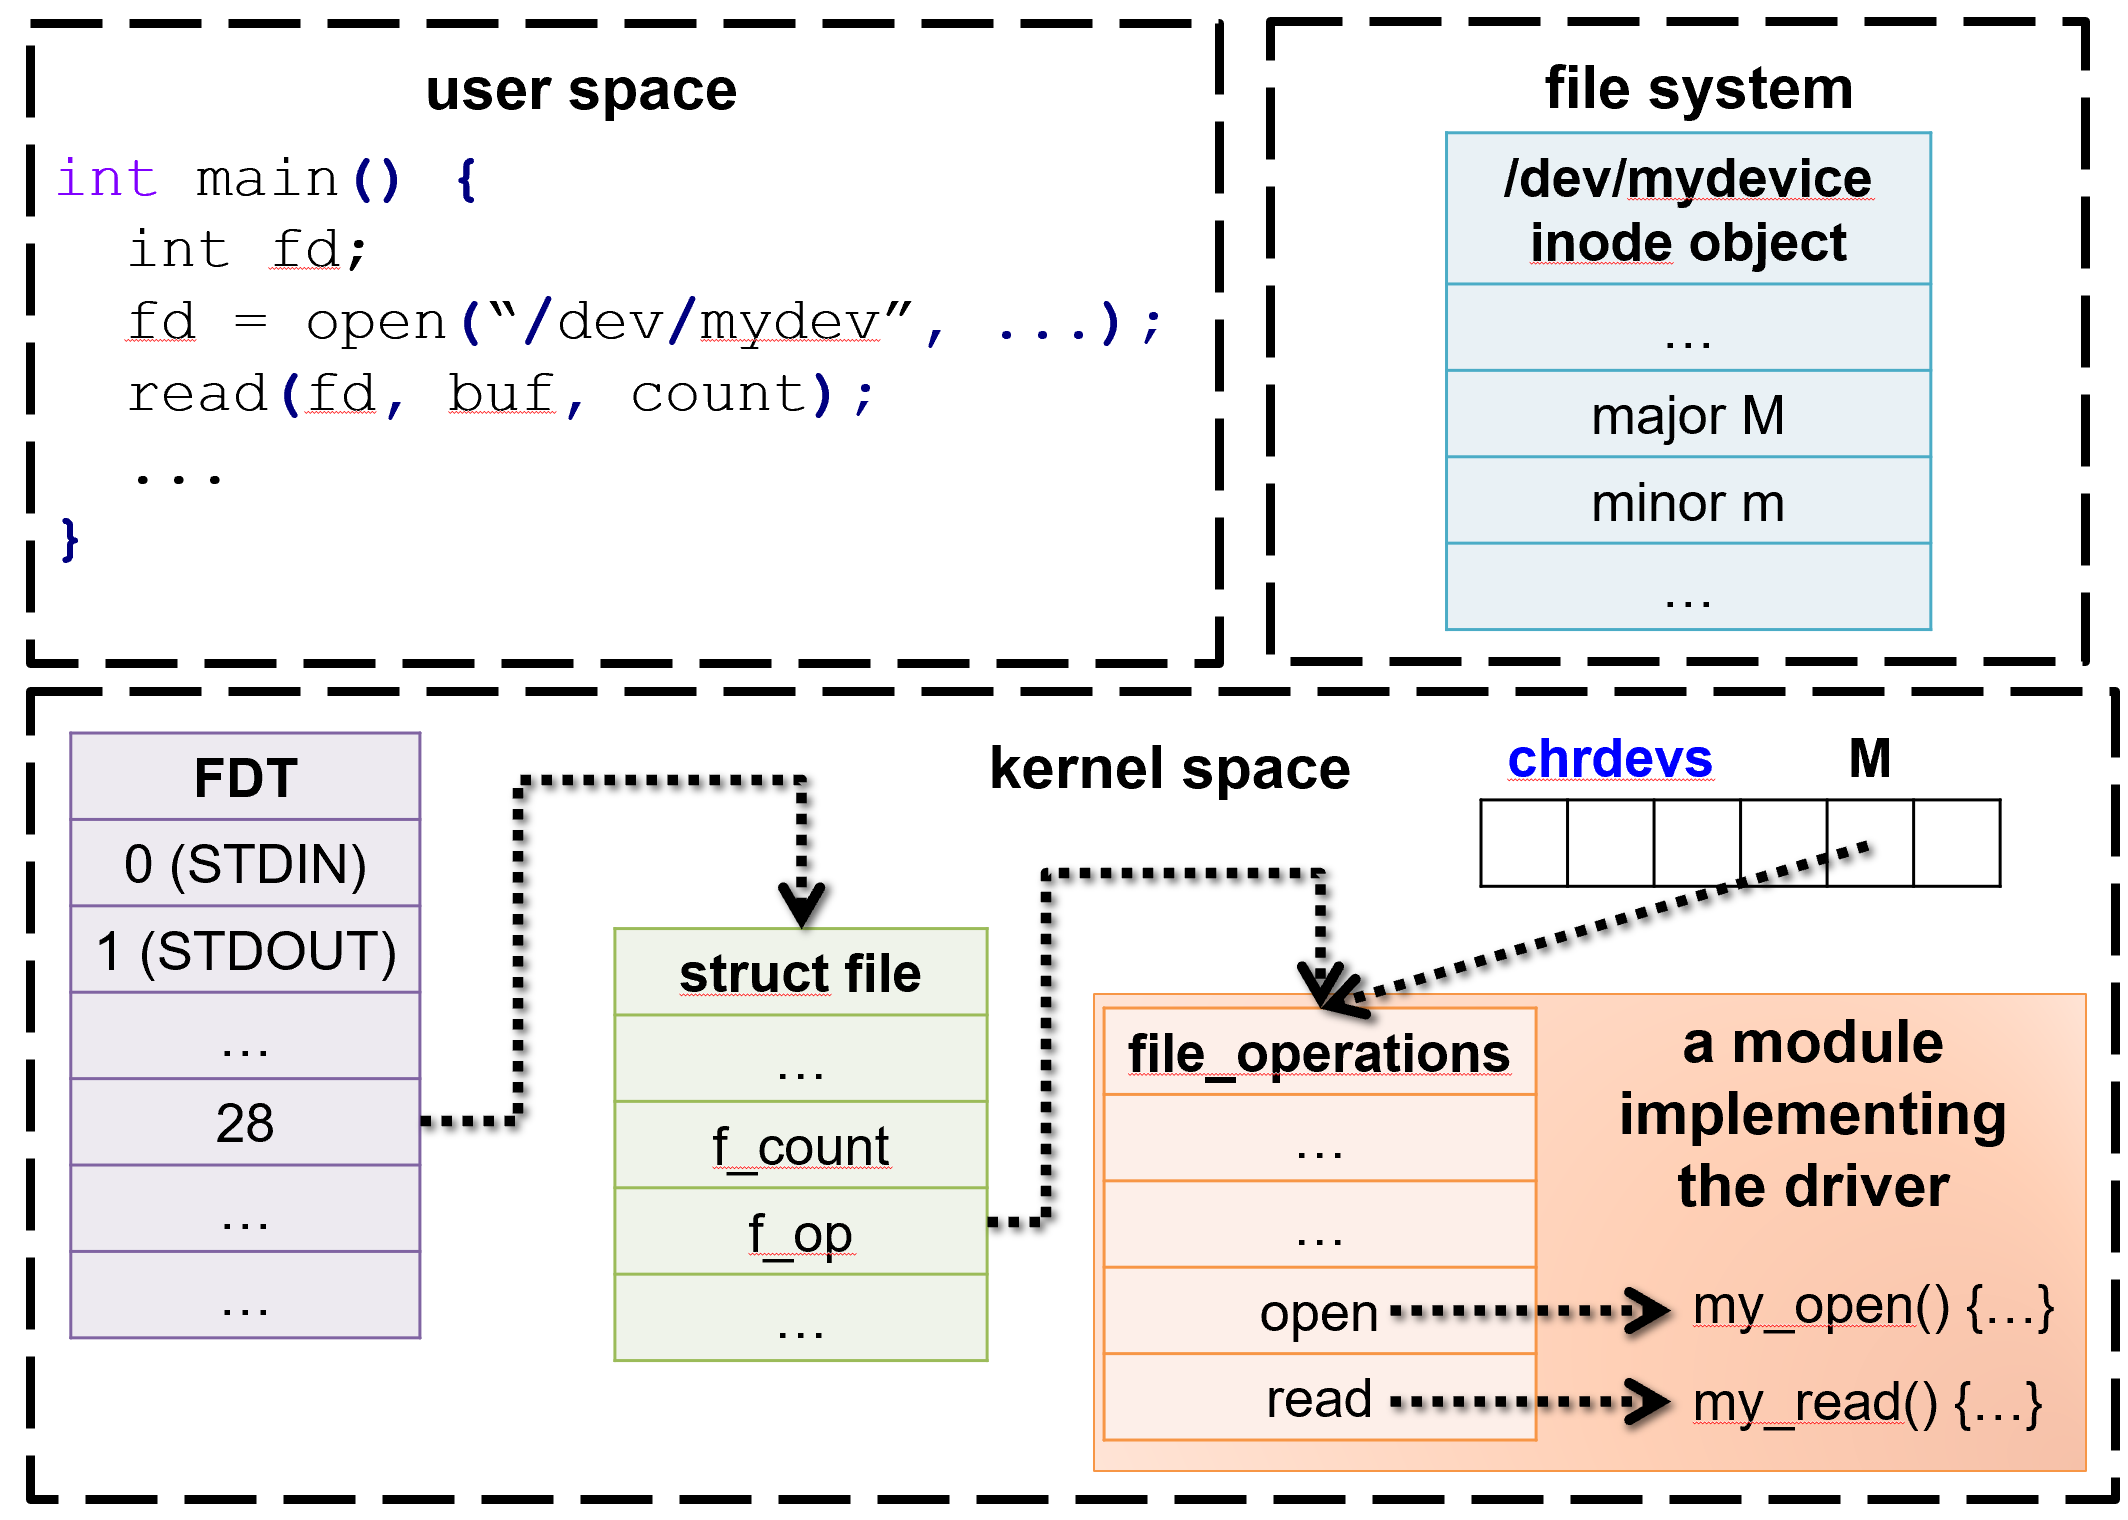
\includegraphics[width=\textwidth]{module_file.png}
    \caption{Module File Flow}
    \label{fig:module_file_flow}
  \end{subfigure}
  \caption{Driver and Module File Flows}
\end{figure}


\paragraph{Registering a Driver} 
To register a driver, we use the \code{register\_chrdev()} function, which adds the driver to the kernel's array of character drivers, \blue{\code{chrdevs[]}}, where the index is the \blue{major} number. It also adds the driver to \code{/proc/devices} file, which lists all registered drivers and their major numbers \gray{(both character \& block drivers)}, character \& block devices use different arrays thus multiples of the same number can exist. \code{chrdevs[]} is an array of driver names + pointers to their \code{file\_ops} structs.


To allocate a major number, Linux allows 512 number options, and each driver can register itself with a major number of its choice (could cause conflicts), or could use \(0\) which then returns the first available number from 512 to 1.


Unregistering a driver using \code{unregister\_chrdev()} will remove the driver from \code{chrdevs[]}, \red{but will not} remove the device from \code{/dev}. 



% =====================================================
% ================== Lecture 4 ========================
% =====================================================


\newpage
\Topic{Scheduling}
\section*{Batch (Non-Preemptive) Scheduling}

\paragraph{Supercomputers} Supercomputers are compromised of multiple nodes, each with multiple CPU cores, and are used for running large-scale computations. Users submit \textbf{batch jobs} to the supercomputer with a specified time limit and size.
Terminology:
\begin{itemize}
  \item \textbf{Size} = the number of CPU cores to use for the job. Jobs are said to be \textit{wide/big} or \textit{narrow/small}.

  \item \textbf{Runtime} = the time limit for the job to run. Jobs are said to be \textit{short} or \textit{long}.
\end{itemize}

\paragraph{Metrics for Performance Evaluation}
When evaluating the performance of a \underline{batch} scheduling algorithm, we use the following metrics:
\begin{itemize}
  \item \textbf{Average Wait Time:} The wait time of a job is the interval between the time the job is submitted to the time the job starts to run. i.e.
        \begin{equation*}
          \text{waitTime} = \text{startTime} - \text{submitTime}
        \end{equation*}

  \item \textbf{Average Response Time:} The response time of a job is the interval between the time the job is submitted to the time the job is terminated. i.e.
        \begin{equation*}
          \text{responseTime} = \text{terminateTime} - \text{submitTime}
        \end{equation*}

        \red{\textbf{Note:}} Average wait time and response time differ only by a constant factor, which is the job's average runtime.

  \item \textbf{The Slowdown / Expansion Factor:} The ratio between a job's response time and its runtime. i.e.
        \begin{equation*}
          \begin{aligned}
            \text{slowdown} & = \frac{\text{responseTime}}{\text{runtime}}                \\
                            & = \frac{(\text{waitTime} + \text{runtime})}{\text{runtime}} \\
                            & = 1 + \frac{\text{waitTime}}{\text{runtime}}
          \end{aligned}
        \end{equation*}

  \item \textbf{Utilization:} The percentage of time the resource (CPU) is busy.

  \item \textbf{Throughput:} How much work is done in one time unit.
\end{itemize}


\subsection*{Batch Scheduling Algorithms}
\begin{center}
  \begin{minipage}{0.30\textwidth}
    \vspace{0pt} % force top alignment
    \centering
    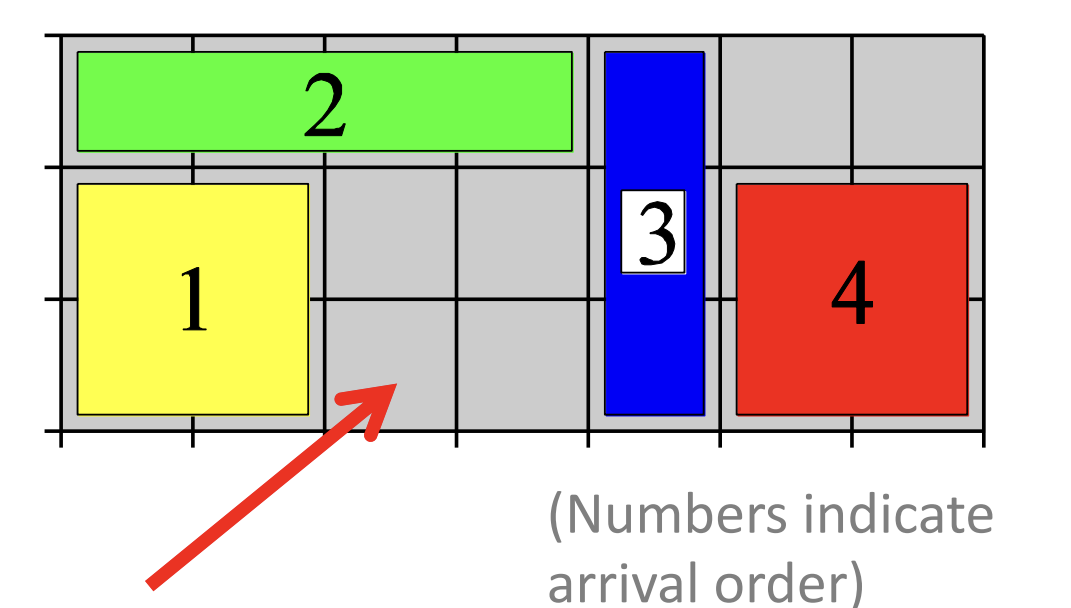
\includegraphics[width=\linewidth]{FCFS.png}
  \end{minipage}\hfill
  \begin{minipage}{0.65\textwidth}
    \vspace{0pt} % force top alignment 
    \paragraph{First-Come, First-Served (FCFS)} Jobs are scheduled by their arrival time. If there are enough free cores, a newly arriving job starts to run immediately, otherwise it wait, sorted by arrival time, until enough cores are available.
    \begin{itemize}
      \item \textbf{Pros:} Simple to implement (FIFO Queue), fair to all jobs.
      \item \textbf{Cons:} Creates \textit{\ul{fragmenation}}, small/short jobs might wait a long time.
    \end{itemize}
  \end{minipage}
\end{center}

\noindent\rule{\linewidth}{0.4pt}


\begin{center}
  \begin{minipage}{0.65\textwidth}
    \vspace{0pt} % force top alignment
    \paragraph{EASY Scheduling (= FCFS + backfilling)} Backfilling optimization: A short waiting job can jump over the head of the wait queue (i.e. start at an earlier time) provided that \red{it doesn't delay} the job \@ head of the FCFS queue.\\

    The algorithm: whenever a job arrives or terminates, try to start the job \@ head of the FCFS wait queue. Then, iterate over the rest of teh waiting jobs (in FCFS order) and try to backfill them.

    \begin{itemize}
      \item \textbf{Pros:} Better utilization (less fragmentation), short jobs have a better chance of running sooner.
      \item \textbf{Cons:} Must know runtimes in advance.
    \end{itemize}
  \end{minipage}\hfill
  \begin{minipage}{0.3\textwidth}
    \vspace{0pt} % force top alignment 
    \centering
    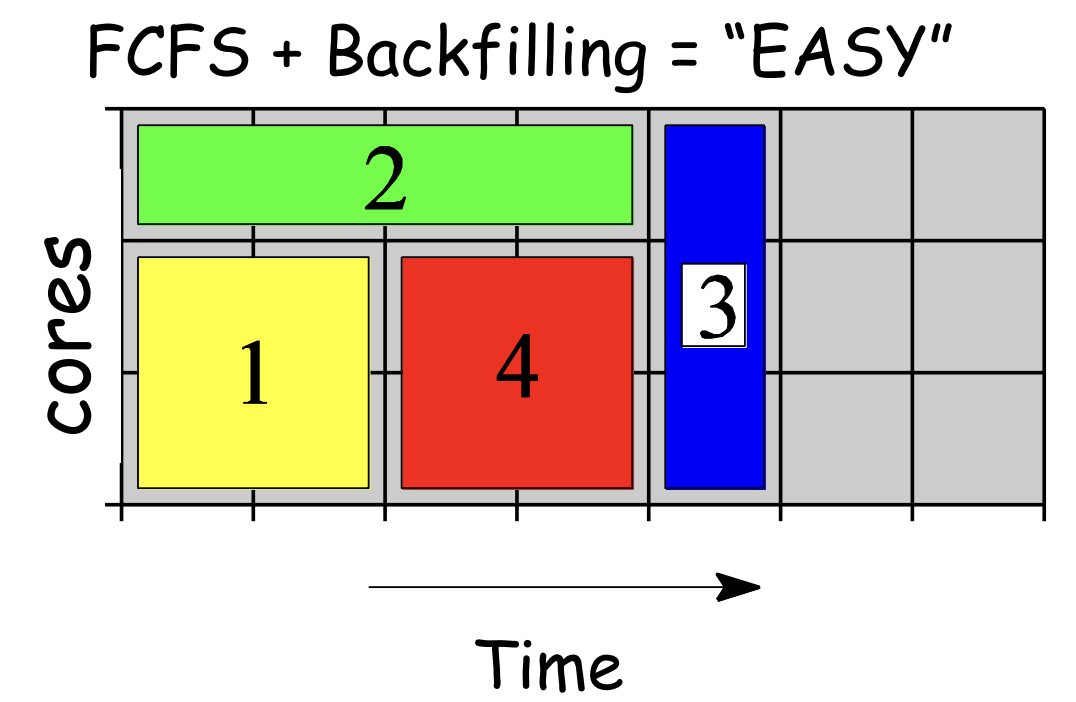
\includegraphics[width=\linewidth]{EASY.png}
  \end{minipage}
\end{center}

\noindent\rule{\linewidth}{0.4pt}


\paragraph{Shortest Job First (SJF)} Instead of ordering jobs by their arrival time, we order them by \blue{their (typically estimated) runtimes}.
\begin{itemize}
  \item \textbf{Pros:} \red{Optimal} in terms of performance (min. avg. wait time).
  \item \textbf{Cons:} Unfair as it may cause \textbf{starvation} of long jobs. \gray{starvation = can theorically wait forever}
\end{itemize}

\noindent\rule{\linewidth}{0.4pt}



\paragraph{Convoy Effect} Slowing down all \gray{(possibly short)} processes due to currently servicing a very long process. \textit{FCFS} suffers from this effect, as does \textit{EASY} scheduling but to a lesser extent. \textit{SJF} \red{without assumptions} also suffers from this effect but to an even lesser extent.

\begin{samepage}
  \paragraph{Optimality of SJF} As mentioned above, SJF is optimal in terms of performance, in particular, it minimizes the average wait time. \blue{\textbf{Claim:}}\\
  Given:
  \begin{enumerate}
    \item A 1-core system where all jobs are serial.
    \item All process arrive together.
    \item Their runtimes are known in advance.
  \end{enumerate}
  Then: \textit{The average wait time of SJF is equal to or less than the average wait time of any other batch scheduling order.}
\end{samepage}


\paragraph{Fairer Varients of SJF} Motivation: disallow job starvation.
\begin{itemize}
  \item \textbf{Shortest-Job Backfilled First (SJBF):} Exactly like EASY in terms of servicing the head of the wait queue in FCFS order (and not allowing anyone to delay it), but the \textit{backfilling} traversal is done in SJF order, i.e. the next job to be backfilled is the one with the shortest estimated runtime.

  \item \textbf{Largest eXpansion Factor (LXF):} LXF is similar to EASY, but instead of ordering the wait queue in FCFS, it orders jobs based on their current slowdown \red{(greater slowdown = higher priority)}.

        \indent On every job arrival or termination, the expansion factors are recalculated and the wait queue is resorted, so that the job with the largest expansion factor is always at the head of the queue. Both the head of the queue and the backfilled jobs are serviced in LXF order.
\end{itemize}



\newpage
\section*{Preemptive Schedulers}
\paragraph{Preemption} \textit{is the act of suspending one job (process) in favor of another even though it is not finished yet.}

Why do we need preemption? Preemption is necessary for \textbf{responsiveness} and when the runtime of jobs vary or unknown in advance.

\paragraph{Quantum} \textit{is the maximum amount of time a process is allowed to run before it is preempted.} Quantum is typically milliseconds to 10s of milliseconds, and is \textit{often set per-process}. Usually a CPU-bound process gets long quanta while an I/O-bound process gets short quanta with higher priority.

\paragraph{Performance Metrics for Preemptive Schedulers} we use the following:
\begin{itemize}
  \item \textbf{Average Wait Time:} As before, the wait time of a job is the interval between the time the job \textbf{is submitted} to the time the job \textbf{starts to run}. \textit{Note} that the wait time \red{does not include} the preemption wait times (i.e. the time the job is waiting for its turn to run again after being preempted).

  \item \textbf{Response Time (=Turnaround Time):} Like before, the response time is the time from process submission to process completion. \textit{Note} that with preemption we get:
        \begin{equation*}
          \text{responseTime} \geq \text{waitTime} + \text{runtime}
        \end{equation*}
        due to the preemption wait times and \textbf{Context Switches} cost.

  \item \textbf{Overhead:} How long a context switch takes, and how often context switches happen. (Should be minimized)

  \item \textbf{Utilization \& Throughput:} Same as before, but we may want to account for context switch overhead.

  \item \textbf{Makespan Time:} The time it takes for the system to finish all jobs in the system.

\end{itemize}


\paragraph{Round Robin (RR) Scheduling} \textit{Processes are arranged in a cyclic read-queue}. The algorithm works in the following steps:
\begin{enumerate}
  \item  The head process runs until its quantum is exhausted.
  \item The head process is then preempted (suspended) and moved to the tail of the queue.
  \item The scheduler resumes the next process in the circular list.
  \item When we've cycled through all processes in the run-list (and we reach the head process again), we say that the current \textbf{"epoch"} is over, and the next epoch begins.
\end{enumerate}
\textbf{Note:} RR Requires a timer interrupt; Typically it's a periodic interrupt (fires every few milliseconds) and upon receiving the interrupt, the OS checks if its time to preempt.
\textbf{Note 2:} For \ul{small enough} quantum, it's like everyone of the N processes advances in \(1/N\) of the speed of the core \gray{called sometimes virtual time}.
With \ul{huge} quantum \gray{infinity}, RR becomes FCFS.

\paragraph{Gang Scheduling} Think of it as RR for \textit{parallel} systems. It works as follows:
\begin{itemize}
  \item Time is divided to slots (seconds or minutes).
  \item Every job has a \textbf{"native"} time slot.
  \item Algorithm attempts to fill holes in time slots by assigning to them jobs from other native slots (called \textbf{"alternative"} slots).
  \item Algorithm attempts to minimize slot number using \textbf{slot unification} when possible.
  \item Rarely used in practice, if lots of memory is swapped out upon context switch, context switch overhead is too high.
\end{itemize}
Detailed explanation about alternative slots and slot unification:

\paragraph{Alternative Slots} To further enhance resource utilization, the gang scheduling algorithm attempts to fill holes in time slots. A job has a "native" time slot where it is primarily scheduled to run. However, if there are idle processors in other time slots (termed "alternative" slots), the scheduler can assign jobs from their native slots to run in these otherwise unused resources. This allows jobs to get more processing time without interfering with the primary scheduling of other jobs.

\paragraph{Slot Unification}This technique aims to minimize the total number of active time slots. If, after some jobs have completed, the remaining jobs in two different time slots can fit into a single slot without conflict, the scheduler can merge them. By unifying slots, the overall cycle time of the matrix is reduced, which can lead to shorter job turnaround times and improved system throughput.

\begin{figure}[H]
  \centering
  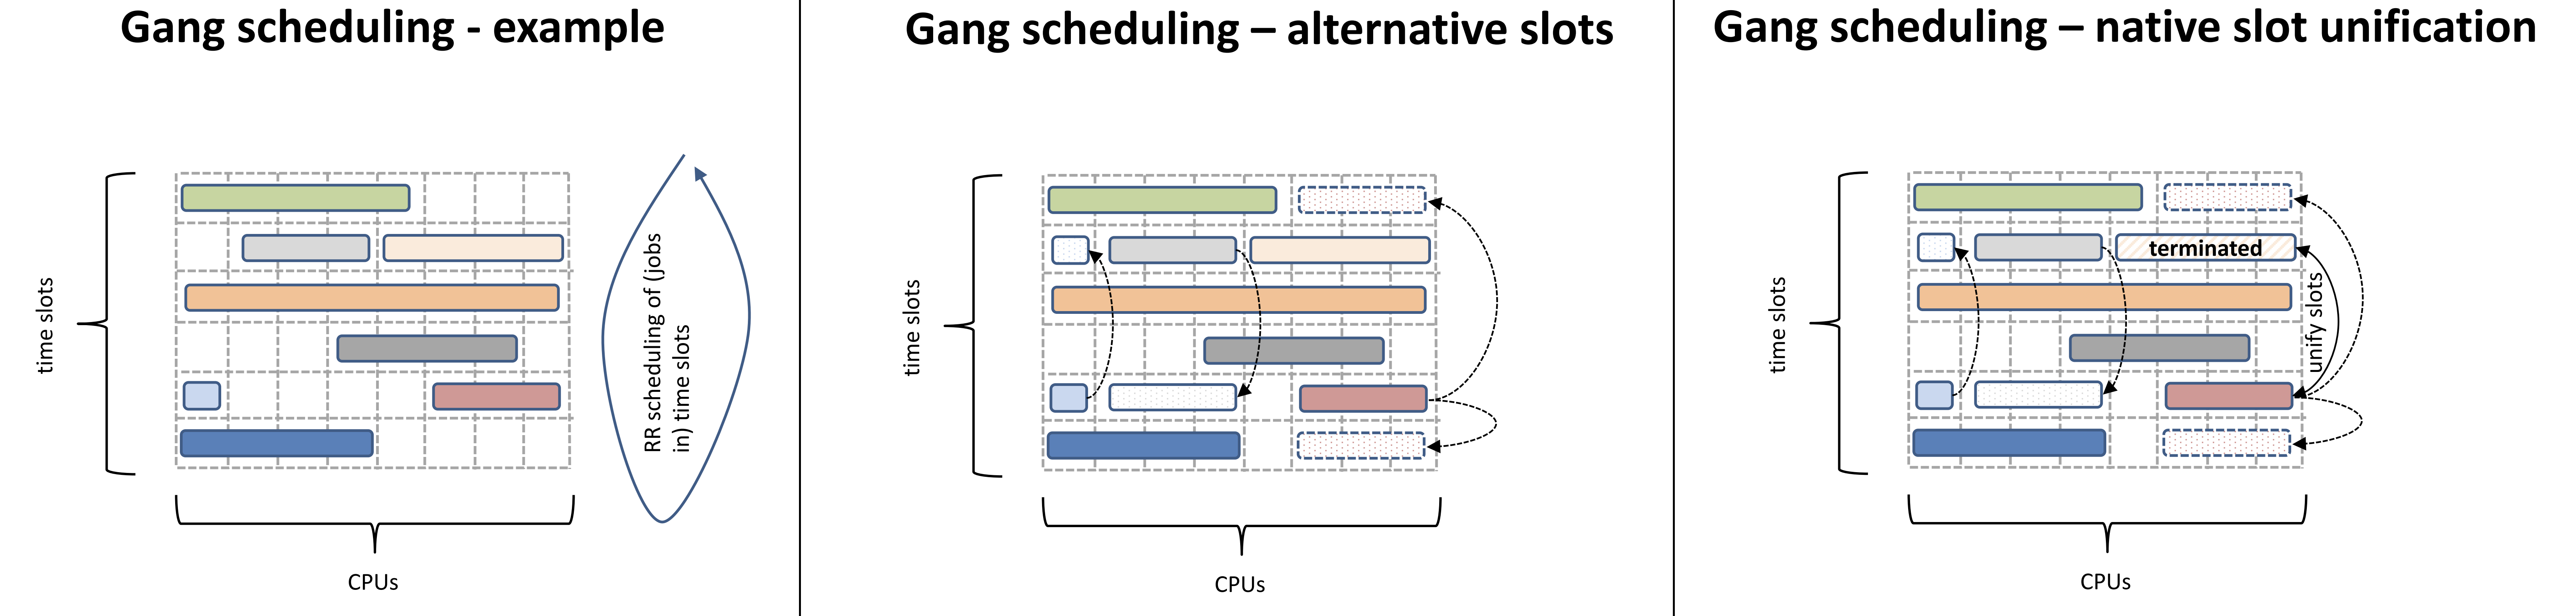
\includegraphics[width=1\textwidth]{GangScheduling.png}
  \caption{Gang Scheduling}
  \label{fig:Gang_Scheduling}
\end{figure}


\begin{samepage}
  \paragraph{Batching vs. Preemption} \textbf{Assume:} (1) A single core system (2) All jobs arrive together (3) Context switch price = 0. \textbf{Then:} There \ul{exists} a non-preemptive algorithm such that:
  \begin{equation*}
    \text{avgResponseTime}(\text{non-preemptive}) \leq \text{avgResponseTime}(\text{preemptive})
  \end{equation*}
  As a result, SJF is also optimal relative to preemptive scheduling (if our assumptions hold).
  \begin{equation*}
    \text{avgResponseTime}(\text{SJF}) \leq \text{avgResponseTime}(\text{batch or preemptive scheduler})
  \end{equation*}
\end{samepage}


\paragraph{Connection Between RR \& SJF} \textbf{Assume:} (1) A single core system (2) All jobs arrive together \gray{(and only use CPU, no I/O)} (3) Quantum is uniform + \red{no} context switch overhead. \textbf{Then:}
\begin{equation*}
  \text{avgResponse}(\text{RR}) \leq 2\cdot \text{avgResponse}(\text{SJF})
\end{equation*}
i.e. RR at best is as good as SJF, and at worst is \(2X\) slower.


\paragraph{Shortest Remaining Time First (SRTF)} If we remove the assumption that all jobs arrive together, then SJF is not optimal anymore, as it may cause a convoy effect. \textbf{SRTF} is a preemptive version of SJF, where the scheduler always runs the job with the shortest remaining time. i.e. when a new job arrives or an old one finishes, the scheduler runs the job with the shortest remaining time, even if it means preempting the currently running job. This is \ul{optimal} in terms of average response time, but it can cause starvation for long jobs.


\paragraph{Selfish RR} Selfish RR is a variant of RR where only "old enough" processes are running in the run-queue. i.e.
\begin{itemize}
  \item New processes wait in a FIFO queue, not yet scheduled.
  \item Older processes scheduled using RR.
  \item New processes are scheduled when either of the following happens:
        \begin{enumerate}
          \item The run-queue is empty (i.e. no ready-to-run "old" processes exist).
          \item "Aging" is being applied to new processes \gray{(a per-process counter increases over time)}; When the counter passes a certain threshold, the "new" process becomes "old" and is transferred to the RR queue.
        \end{enumerate}
  \item \textbf{Fast Aging} = Algorithm resembles RR, \textbf{Slow Aging} = Algorithm resembles FCFS.
\end{itemize}


\section*{General Purpose Schedulers (Priority-Based \& Preemptive)}

\paragraph{Scheduling using priority} Every process is assigned a priority. The priority reflects how "important" it is in that time instance, and it changes dynamically over time. Process with higher priority are favored, as they are scheduled before lower priority processes. The concept of priority can be also applied in batch scheduling. e.g. SJF:priority = runtime (smaller runtime = higher priority), FCFS:priority = arrival time (earlier arrival = higher priority), etc.

\paragraph{Negative Feedback Principle} The schedulers of all general-purpose OSes employ a negative feedback policy: \ul{Running reduces priority to run more} \& \ul{Not running increases priority to run}.
As a result, I/O-bound processes (that seldom use the CPU) get higher priority than CPU-bound processes (that use the CPU a lot). This ensures that I/O-bound processes are responsive.

\paragraph{Multi-Level Priority Queue} A multi-level priority queue consists of several RR queues, each associated with a priority. processes migrate between the queues so they have a dynamic priority, "important" processes move up (e.g. I/O-bound) and "unimportant" processes move down (e.g. CPU-bound). Priority is greatly affected by the \textbf{negative feedback principle}, i.e. by CPU consumption:
\begin{itemize}
  \item I/O-bound \(\Longleftrightarrow\) move up
  \item CPU-bound \(\Longleftrightarrow\) move down
\end{itemize}
Some schedulers allocate short quanta to higher priority queues, and some don't or even do the opposite.



\section*{Linux \(\leq\) 2.4 Scheduler}
All of the definitions below are relative only to the Linux \(\leq\) 2.4 scheduler, which is a preemptive priority-based scheduler that uses a multi-level priority queue. \textbf{Note:} A task is either a process or a thread.

\paragraph{Standard POSIX Scheduling Policies} POSIX dictates that each task is associated with one of three scheduling policies:
\begin{itemize}
  \item \textbf{"Realtime"} Policies:
        \begin{enumerate}
          \item \code{SCHED\_RR} (round-robin): The time slice is calculated as \((100 * HZ)/ 1000\) \gray{HZ = number of times interrupts per second}.
          \item \code{SCHED\_FIFO} (first-in, first-out): doesn't give up the CPU unless: (1) voluntarily using \code{sched\_yeild()}, (2) I/O operation, (3) preempted by a higher priority task.
        \end{enumerate}
  \item The default policy:
        \begin{enumerate}
          \setcounter{enumi}{2}
          \item \code{SCHED\_OTHER} (the default time-sharing policy)
        \end{enumerate}
\end{itemize}
POSIX defines the meaning of \code{SCHED\_OTHER} (aka \code{SCHED\_NORMAL} in Linux) is decided by the OS. Typically employs some multi-level priority queue with the negative feedback loop.

\vspace*{1em}

\textit{Realtime} tasks are \blue{always favored} by the scheduler. Only an \ul{admin} can set a task to run with a \textit{realtime} policy, the users can set a policy using the \code{sched\_setscheduler} syscall. The multi-level priority queue is leveled from 0-99: \ul{In kernel} - 0 is the highest, \ul{In user} - 99 is the highest (e.g. syscalls), as kernel calculates (99-input).




\paragraph{Epoch} As mentioned before,every runnable task gets allocated a quantum, which is the CPU time the task is allowed to consume before is it's stopped by the OS. Whenever all quanta of all \textit{runnable} tasks become zero a \textbf{new epoch} begins. In this case we allocate additional running time to \textit{all tasks} (runnable or not).

\subsection*{Definitions}
\begin{itemize}
  \item \textbf{Task's Priority:} Every task is associated with an integer, the higher the value the higher the priority to run. Every task has a \textit{static} priority and a \textit{dynamic} priority.
  \item \textbf{Static Priority:} A fixed value that indirectly determines the maximal quantum for the task. Fixed unless the user invokes \code{nice()} or \code{sched\_setscheduler} syscalls.
  \item \textbf{Dynamic Priority:} Is the both the \blue{remaining time} for the task and its \blue{current priority}. The dynamic priority decreases over time (while running), if it reaches zero the task is preempted until the next epoch. The dynamic priority is \textit{reset} to the static priority at the beginning of each epoch.

  \item \textbf{HZ:} Linux gets a timer interrupt \textit{HZ} times per second, i.e. it gets a timer interrupt every \(\frac{1}{\textit{HZ}}\) seconds. The default value of \textit{HZ} is 100 for x86/Linux2.4.

  \item \textbf{Tick:} A tick can mean either of the following:
        \begin{itemize}
          \item The time that elapses between two consecutive timer interrupts, i.e. \(\frac{1}{\textit{HZ}}\) seconds.
          \item The timer interrupt itself that fires every \(\frac{1}{\textit{HZ}}\) seconds.
        \end{itemize}
        Ticks are used to determine the scheduler timing resolution, the OS measures the passage of time in ticks. The units of the \textit{dynamic priority} are ticks.

  \item \textbf{task\_struct:} Every task is represented by a \textit{task\_struct} object, which contains (among other things):
        \begin{enumerate}
          \item nice \gray{static priority}
          \item counter \gray{dynamic priority}
          \item processor \gray{the last CPU core the task ran on}
          \item need\_resched \gray{boolean}
          \item mm \gray{task's memory address space}
        \end{enumerate}

  \item \textbf{task's nice} There are two types of nice, user nice and kernel nice. The \textbf{kernel's nice} is the \textit{static priority} of the task, which is \blue{between 1...40} (higher is better) and the \blue{default is 20}. The \textbf{user's nice} is the parameter passed to the \code{nice()} syscall, which is \blue{between -20...19} (\red{lower} is better). Values below 0 require superuser privileges.
        \begin{equation*}
          \text{kernel\_nice} = 20 - \text{user\_nice}
        \end{equation*}

        \begin{samepage}
          \item {\textbf{task's counter}} The \textit{dynamic priority} of the task. It is calculated as follows:
          \begin{itemize}
            \item Upon task creation:
                  \begin{equation*}
                    \begin{aligned}
                      \text{child.counter}  & = \text{parent.counter}/2; & \gray{\text{(round down)}} \\
                      \text{parent.counter} & -= \text{child.counter};   & \gray{\text{(round up)}}
                    \end{aligned}
                  \end{equation*}
            \item Upon a new epoch:
                  \begin{equation*}
                    \begin{aligned}
                      \text{task.counter} & = \text{task.counter}/2 + \text{NICE\_TO\_TICKS}(\text{task.nice}) \\
                                          & \gray{= \text{half of prev dynamic + convert\_to\_ticks(static)}}
                    \end{aligned}
                  \end{equation*}
            \item When running: decrement each tick by 1 (task.counter--) until it reaches 0.
          \end{itemize}
          The \textbf{NICE\_TO\_TICKS} function scales 20 (=DEF\_PRIORITY) to number of tick compromising \textbf{50+ ms}. By default, scales 20 to 5+ ticks:\\
          \code{\#define NICE\_TO\_TICKS(kern\_nice) ((kern\_nice) / 4 + 1)}\\
          So the quantum range is therefore: \gray{(recall that 1 tick = 10 ms)}
          \begin{itemize}
            \item (1/4 + 1=) 1 tick = 10 ms (min.)
            \item (20/4 + 1=) 6 ticks = 60 ms (default)
            \item (40/4 + 1=) 11 ticks = 110 ms (max.)
          \end{itemize}

        \end{samepage}

  \item \textbf{task's processor} Logical ID of CPU core upon which task has executed most recently, if task is currently running, then this is the core it is running on.

  \item \textbf{task's need\_resched} A boolean flag that is checked by kernel just before switching back to user-mode. If set, check if there's a "better" task than the one currently running, and if so, switch to it. Can be thought of as a per-core rather than per-task flag as it is checked only for the currently running task.

  \item \textbf{task's mm} A pointer to the task's memory address space. \gray{(More details in the virtual memory lectures)}
\end{itemize}


The scheduler is implemented in the \code{kernel/sched.c} file, and the task structure is defined in \code{include/linux/sched.h}. The scheduler is compromised of \textbf{4 main functions}:
\begin{enumerate}
  \item \code{goodness(task, cpu)} - Given a task and a CPU core, returns how "desirable" it is for that CPU. We compare tasks by this value to determine which task to run next.
  \item \code{schedule()} - Actual implementation of the scheduler. Uses \code{goodness} to decide which task to run on a given core.
  \item \code{\_\_wake\_up\_common(wait\_queue q)} - Wakes up task(s) when waited-for event has happened. e.g. completion of I/O operation, or a signal being sent to the task.
  \item \code{reschedule\_idle(task t)} - Given a task, check whether it can be scheduled on some core. Preferably on an idle core, but if not then by preempting a less "desirable" task on a busy core. \blue{Note:} used by the \code{schedule()} \& \code{\_\_wake\_up\_common()} functions.
\end{enumerate}

\paragraph{Counter Convergence} \textbf{Claim:} The counter value of an I/O-bound task will quickly converge to \(2\alpha\) \gray{geometric series}.
\textbf{Corollary:} By default, an I/O-bound task will have a counter of 12 ticks (=120 ms) \gray{as long as it remains I/O-bound and consumes neglligble CPU time}.

\paragraph{The Drawback} The scheduler is a linear scheduler, i.e. it runs in \(O(n)\) time. It was replaced by the "\(O(1)\)" scheduler which then was replaced by the "\textit{Completely Fair Scheduler}" (CFS) which is \(O(\log n)\).







\section*{CFS (Completely Fair Scheduler)}

\paragraph{CFS} The CFS is a preemptive, priority-based scheduler that aims to provide a fair distribution of CPU time among all tasks while maintaining efficiency and scalability (\(O(\log N)\)).


\paragraph{\code{vruntime} - Virtual Run Time} Every running task obtains virtual run-time. Ideally all tasks maintain an equal amount of virtual run time, and that's the goal. The algorithm stores the minimum \& maximum virtual run times at all times. The minimal virtual runtime task is always the next task to run.


\paragraph{\code{sched\_latency}} The CFS uses a \textit{sched\_latency} parameter to determine the length of an epoch (48 ms). Each task gets a quantum of \(Q_i=\text{sched\_latency}/N\), where N is the number of tasks.


The algorithm also defines a minimum quantum length, \code{sched\_min\_granularity}, which is the smallest time slice a task can receive (6 ms). So in practice, tasks can have a longer epoch than defined by \code{sched\_latency}.


\paragraph{CFS Algorithm} The CFS uses a red-black tree (similar to AVL tree) to maintain the tasks in the system, ordered by their \code{vruntime}. New tasks are inserted into the tree, with their \code{vruntime} set to the \red{\code{max\_vruntime}}. Tasks that come back from I/O operations or are woken up have their \code{vruntime} set to the \red{\code{min\_vruntime}}. 


\paragraph{CFS Priorities \& Weights} The CFS uses a priority system based on the \textit{nice} value of the task. The \code{vruntime} is adjusted based on the task's priority, with higher priority tasks gaining lower \code{vruntime}. The \blue{lower} the nice the \blue{higher} the priority, and for each nice value, there is a corresponding weight (high weight for high priority)

Let \(W_0\) be the weight of nice=0, then:
\[
{VR}_i = \frac{W_0}{W_i} \cdot \Delta T
\]
\[
Q_i = \frac{W_i}{\sum_k W_k} \cdot \text{sched\_latency}
\]








% =====================================================
% ================= Context Switch ====================
% =====================================================


\Topic{Context Switch}


\begin{tabularx}{\textwidth}{|X|X|}
\hline
\multicolumn{1}{|c|}{\textbf{Caller Rules}} & \multicolumn{1}{c|}{\textbf{Callee Rules}} \\
\hline
 & \\
\textbf{Before the function call:} & \textbf{On function entry:} \\
\begin{itemize}
    \item Save caller-saved registers on the stack (\texttt{rax, rcx, rdx, rdi, rsi, r8–r11}).
    \item Pass the first 6 arguments in registers (from left to right: \texttt{rdi, rsi, rdx, rcx, r8, r9}).
    \item Pass the rest of the arguments (beyond the first six) on the stack.
    \item Use the \texttt{call} machine instruction.
\end{itemize}
&
\begin{itemize}
    \item Create a new stack frame (save the old \texttt{rbp} and point to the new top of the stack).
    \item Allocate space for local variables.
    \item Save callee-saved registers on the stack (\texttt{rbx, r12–r15}).
\end{itemize}
\\
\textbf{Upon return from the function:} & \textbf{On function exit:} \\
\begin{itemize}
    \item Restore the saved registers.
\end{itemize}
&
\begin{itemize}
    \item Place the return value in the \texttt{rax} register.
    \item Restore the saved registers.
    \item Deallocate local variables.
    \item Return to the old stack frame (restore the previously saved \texttt{rbp}).
    \item Use the \texttt{ret} machine instruction.
\end{itemize}
\\
\hline
\end{tabularx}

{\centering Two types of context switches:}

\begin{tabularx}{\textwidth}{|X|X|}
\hline
\multicolumn{1}{|c|}{\textbf{Forced Context Switch (Preemption)}} & \multicolumn{1}{c|}{\textbf{Initiated Context Switch}} \\
\hline
 & \\
The kernel preempts (i.e., forcibly takes) the CPU from the process, for example, following: & The process voluntarily gives up the CPU, for example, by means of: \\
\begin{itemize}
    \item A timer interrupt (\texttt{scheduler\_tick}) which reveals that the time slice allocated to the current process has expired.
    \item An asynchronous event that wakes up a process with a higher priority than the currently running process. \gray{For example: a disk interrupt or the release of a lock for which a process was waiting.}
\end{itemize}
&
\begin{itemize}
    \item A blocking system call (such as \texttt{wait()}, \texttt{read()}, ...), which puts the process into a waiting state.
    \item The \texttt{exit()} system call, which terminates the process.
    \item The \texttt{sched\_yield()} system call -- a dedicated system call to yield the CPU.
\end{itemize}
\\
\hline
\end{tabularx}



\paragraph{Preemption in Kernel} The \gray{(new)} linux kernel is preemptive, meaning that a process running in the kernel can be preempted!


When switching context we switch the kernel stacks of the tasks (each task has a corresponding kernel stack in the kernel space).

The only gateway in linux for context switches is the function \code{schedule()}, which \red{can not} be interrupted.


\paragraph{Context Switch Saving} when a context switch occurs we save:
\begin{itemize}
  \item The stack, heap, code (memory regions) are in the memory space of the process, so they do not need to be backed up.

  \item open files and other data are already residing in the PCB, which is in the memory.

  \item Registers \& flags (the CPU state) are backed up to the kernel stack of the thread on a field called \blue{thread\_struct}.

  \item The base of the kernel stack base is pointed to by \blue{TSS.sp0} (the top of the kernel stack) so it needs to be backed up.
\end{itemize}

\paragraph{TSS (Task State Segment)} is a unique data structure for each CPU core that contains the state of the currently running task. It is pointed to by \blue{TR}, and it contains the \blue{TSS.sp0} field which points to the top of the kernel stack of the currently running task. 

Each PCB contains a \code{thread\_struct} field which contains the state of the task, including the CPU registers, flags, and most importantly, the head of the kernel stack.


To do a context switch we do the following steps:
\begin{enumerate}
  \item \textbf{\code{context\_switch()}}: This function calls for switching the memory space, and calls the next function -

  \item \textbf{\code{\_\_switch\_to\_asm()}}: The macro that saves the current context and loads the next one. More specifically, it backs the registers \& the rsp of the kernel and loads the new one, pops the backed registers (of the new one) and then calls the next function -

  \item \textbf{\_\_switch\_to()}: This function updates the TSS.sp0 field to point to the new kernel stack, and returns to return address of \code{\_\_switch\_to\_asm()} or \code{ret\_from\_fork()}.
\end{enumerate}

\paragraph{\code{do\_fork()}} is the kernel function used by \code{fork()} and \code{clone()} to create the new context of the new thread:
\begin{enumerate}
  \item It allocates a new PCB for the new thread, and a new kernel stack
  \item Calls for \code{copy\_thread()}, which fills the kernel stack of the child process to be as it was the one who called \code{fork()} and then \code{\_\_switch\_to\_asm()}
  \item Copies to the child process most of the PCB fields and data from the father.
  \item Connects the child process to its family connections.
  \item Adds the child process to the global process list. \gray{and to the pid hash table}
  \item Transfers the child task to \code{TASK\_RUNNING} state and adds it to the \code{runqueue}.
  \item The functions returns the pid of the child, and this value is returned from the father too.
\end{enumerate}

\code{copy\_thread()} copies the registers from the parent to the child, sets the \code{rax} register of the child to 0, and updates the return address that is saved on the stack to the \code{ret\_from\_fork()} function, and finally sets the task kernel stack head (rsp) to the new kernel stack of the child process.

\code{ret\_from\_fork()} is the function that pops the registers from the kernel stackand returns to the user code (using \code{sysret})


\paragraph{\code{do\_exit()}} is the function that is called when a process exits (either by calling \code{exit()} or by signals/interrupts). It does the following:
\begin{enumerate}
  \item Frees the resources of the task, closes all open files, frees memory, etc.
  \item Sets the exit value to the \code{exit\_code} field of the PCB.
  \item Updates family ties: all children become orphans (children of init), the parent keeps the pointer to the exiting child, all siblings lose their pointer to the exiting process.
  \item Updates the task state to \code{TASK\_ZOMBIE}
  \item Calls the function \code{schedule()} to run a different task. The task runtime is finished by \code{\_\_switch\_to\_asm()}.
\end{enumerate}









% =====================================================
% ======== Lecture Synchronization ====================
% =====================================================





\newpage
\Topic{Synchoronization (\& Deadlocks)}

\paragraph{\red{Race Condition}} We say that the program suffers from a \textit{race condition} if the \textit{outcome is nondeterministic and depends on teh timing of uncontrollable, un-synchronized events}

\paragraph{Memory (Cache) Coherency} is the mechanism that ensures that any change to a shared piece of data in one cache is eventually propagated to all other caches, preventing processors from working with outdated information.

\paragraph{Cache Consistency} it dictates how memory operations (reads and writes) from one processor can be observed by other processors in the system. If store operations are immediately seen by other cores and they can't be reordered with load operations, then consistency holds. (but it's not a necessary condition)

Cache \textbf{coherency} relates to a \textbf{single} memory location, while cache \textbf{consistency} relates to \textbf{multiple} memory locations. coherency ensures cores see writes in some order that makes sense, and is uniform across all cores. Consistency is about the order of different read and write operations across multiple memory locations, and how they are observed by different cores.

To enforce ordering for memory consistency, explicit \textbf{memory fence} (memory barrier) must be used. The fence makes all store-s that happened before the fence visible to all load-s after the fence, notably, flushes the store buffer to teh memory system.


\paragraph{Atomicy} In programming, atomicity means an operation, or a series of operations, appears to happen all at once, without any interruption from other processes. This ensures that either the entire operation completes successfully, or it has no effect at all, preventing partial or incomplete results. 

In \ul{single core} CPUs each instruction is atomic, i.e. it can't be interrupted by another instruction. In \ul{multi-core} CPUs, atomicity is only achieved by using special instructions or locks that ensure no other thread can access the data while the operation is being performed. (e.g. \code{lock; instruction})


\paragraph{Critical Section} A group of operations we need to atomically execute is called a \textbf{critical section}. Atomicity will make sure other threads don't see partial results! The critical section can be a uniform code across all threads, or it can be a different.

\paragraph{Mutual Exclusion (mutex)} is a property of a critical section that ensures that only one thread can execute it at a time and never simultaneously. Thus a critical section is a \blue{"serilaization point"}.



\section*{Locks}

\paragraph{Lock} A lock is an abstraction that supports two operations: \code{acquire(lock)} and \code{release(lock)}.
Semantically: It's a memory fence, only one thread at a time can acquire the lock and other simultaneous attempts to acquire are postponed until the lock released. Implementing a lock is nowadays done using hardware support with special instructions that ensure mutual exclusion.

\paragraph{Spinlock} A spinlock is a lock that uses busy-waiting to acquire the lock. i.e. it repeatedly checks if the lock is available and only then acquires it. Spinlocks are typically used in low-level code where the overhead of sleeping and waking up is too high, or when the critical section is very short. If interrupt or signal handlers access the same data as the critical section, then the we must disable them, or make sure they acquire the lock too!

\begin{lstlisting}[language=C, caption={Spinlock Implementation}, label={lst:spinlock}]
struct spinlock {
    uint locked; // 0 = unlocked, 1 = locked
};

// The volatile keyword is crucial here. It tells the compiler that the value at addr can be changed by external factors (like another CPU core or hardware) at any time. This prevents the compiler from making optimizations like caching the value in a register, forcing it to read directly from memory every time.
inline uint xchg(volatile uint *addr, uint newval) {
    // atomic [oldval = *addr, swap(*addr, newval)]
    // xchg is atomic
    // lock adds a memory fence
    uint oldval;
    asm volatile("lock; xchg %0, %1"
                 : "+m" (*addr), "=r"(oldval):
                 "1"(newval):
                 "cc");
    return oldval;
}

void acquire(struct spinlock *lock) {
    disable_interrupts();
    while (xchg(&lock->locked, 1) != 0) {
        // busy-wait until the lock is available
        enable_interrupts();  // if we want to enable
        disable_interrupts(); // interrupts while spinning
    }
}

void release(struct spinlock *lock) {
    xchg(&lock->locked, 0); // set the lock to unlocked
    enable_interrupts(); 
}
\end{lstlisting}


\paragraph{Other Atomic Operations} We know of \textbf{3} atomic operations that are used to implement spinlocks:
\begin{enumerate}
  \item \textbf{xchg(addr, newval)} - Atomically exchanges the value at \code{addr} with \code{newval} and returns the old value.

  \item \textbf{test\_and\_set(bool *b)} - Atomically sets \code{*b} to \textit{true} and returns the old value of \code{*b}.

  \item \textbf{cas(int *p, int old\_val, int new\_val)} - (Compare-and-Swap) Atomically compares the value at \code{*p} with \code{old\_val}, and if they are equal, sets \code{*p} to \code{new\_val} and returns true. Otherwise, it returns false and does not change \code{*p}.
\end{enumerate}







\section*{Mutex Lock}



\paragraph{Spinning or Blocking} A lock can be implemented using either \textbf{spinning} or \textbf{blocking}:
\begin{itemize}
  \item \textbf{Spin (busy wait)} - The thread repeatedly checks if the lock is available, consuming CPU cycles while waiting. This is suitable for short critical sections where the wait time is expected to be very short. Note that the user \red{can not} block context switches.

  \item \textbf{Block (go to wait/sleep)} - The thread goes to sleep and is woken up when the lock is available. This is suitable for longer critical sections where the wait time can be significant.
\end{itemize}
Rule of thumb: If the critical section is shorter than the time a context switch takes, then use spinning, otherwise use blocking.\\
Unlike spinning which can be done by the user, going to sleeping is done by a request to the OS (since it involves changing process states).


\paragraph{Mutex interface} the following are the common ops:
\begin{itemize}
  \item \code{mutex\_init(mutex\_t *mutex, const mutex\_attr\_t *att)}: Initializes the mutex object. The \code{att} parameter can be used to set attributes.

  \item \code{mutex\_lock(mutex\_t *mutex)}: Acquires the mutex lock. If the lock is already held by another thread, the calling thread will block until the lock is available.

  \item \code{mutex\_trylock(mutex\_t *mutex)}: Attempts to acquire the mutex lock without blocking. If the lock is available, it acquires it and succeeds. Otherwise if the lock is already held by another thread, it fails and continues.

  \item \code{mutex\_unlock(mutex\_t *mutex)}: Releases the mutex lock. If there are threads waiting for the lock, one of them will be woken up.

  \item \code{mutex\_destroy(mutex\_t *mutex)}: Destroys the mutex object and releases any resources associated with it. The mutex must not be locked when this function is called, otherwise it fails.
\end{itemize}

\paragraph{Undefined Actions} In a correct implementation of a mutex, only the thread that holds the lock can call \code{mutex\_unlock()}. The following are undefined behaviors:
\begin{itemize}
  \item re-locking the mutex by the same thread that holds it.
  \item unlocking the mutex by a thread that does not hold it.
  \item unlocking a mutex that is not locked.
\end{itemize}



\paragraph{Condition Variables} A condition variable is a synchronization primitive that allows threads to wait for certain conditions to be met, while inside a critical code section without the need to block the CPU!
A condition variable is always associated with a mutex, and it allows threads to wait for a condition to be signaled by another thread. The typical usage pattern is as follows:
\begin{itemize}
  \item A thread acquires the mutex lock.
  \item The thread checks the condition. If the condition is not met, it calls \blue{\code{cond\_wait(cond\_var, mutex)}} to release the mutex (it must be held by the thread beforehand) and block until another thread signals the condition variable.
  \item When the condition is met, another thread can call \blue{\code{cond\_signal(cond\_var)}} to wake up one waiting thread or \blue{\code{cond\_broadcast(cond\_var)}} to wake up all waiting threads.
  \item The waiting thread must re-acquire the mutex lock before continuing execution. (part of the \code{cond\_wait()} operation)
  \item The thread should then check the condition again and proceed if it is met.
\end{itemize}

\section*{Semaphores}

\paragraph{The Basics} A semaphore is usually implemented as a counter and a queue of waiting threads. A task that announces it's waiting for a resource will get the resource if it is available or will go to sleep otherwise. In case it goes to sleep it will be awakened when the resource becomes available to it.

The fields of the semaphore are as follows:
\begin{itemize}
  \item Value (integer) \gray{(the counter)}:\par
        If value is Non-negative, it indicates the number of available resources. If value is negative, it indicates the number of tasks waiting for the resource.

  \item A queue of waiting task: \par
        Every task that is waiting for the resource to become available is stored in this queue. When the value is negative, \(|\text{value}| = \text{queue.lenght}|\)/

\end{itemize}


The functions used to manipulate the semaphore are:
\begin{itemize}
  \item \code{wait(sem)}: Decrements the value of the semaphore. If the value \gray{after decrementing} is negative, the task goes to sleep and is added to the queue of waiting tasks. Otherwise, it continues execution.

  \item \code{signal(sem)}: Increments the value of the semaphore. If the value was negative before incrementing, it wakes up one task from the queue of waiting tasks.
\end{itemize}

\paragraph{Semaphore Implementation} The semaphore is implemented in the kernel and \red{not} part of the course material. However, the following is a demonstration of the problem known as \red{\textbf{lost wakeups}}.
\begin{lstlisting}[language=C, caption={Lost Wakeups Problem}, label={lst:lost_wakeups}]
struct semaphore_t {
    int value;                          
    wait_queue_t wait_queue;            
    lock_t lock;                        
};

void wait(semaphore_t *sem) {
    lock(&sem->lock);
    sem->value--; 
    if (sem->value < 0) {
        enque(self, &sem->wait_queue);
        unlock(&sem->lock);             // This is the problem!
        block(self);
    } else 
        unlock(&sem->lock);
}

void signal(semaphore_t *sem) {
    lock(&sem->lock);
    sem->value++;
    if (sem->value <= 0) {
        p = dequeue(&sem->wait_queue); // Part of the problem too!
        wakeup(p);
    }
}
\end{lstlisting}
The problem with the above implementation is that we release the the lock before going to sleep but after joining the queue, so if another task calls \code{signal()} red{before} we go to sleep, it will wake us up (without being asleep) and we \red{will exit} the wait queue so \textit{no one will be able to wake us up again}. This is known as the \textbf{lost wakeups} problem.



\begin{samepage}
  \begin{center}
    \textbf{Spinlock vs. Semaphore}
    \rowcolors{2}{gray!15}{white}
    \begin{tabular}{|>{\raggedright\arraybackslash}p{3cm}|
      >{\raggedright\arraybackslash}p{4cm}|
      >{\raggedright\arraybackslash}p{6cm}|}
      \hline
      \rowcolor{blue!30}
                           & \textbf{spinlock}                                               & \textbf{semaphore}                                                                                                                 \\
      \hline
      wait by              & spinning                                                        & sleeping                                                                                                                           \\
      granularity          & fine                                                            & coarse: might wait for a long time                                                                                                 \\
      complexity           & lower                                                           & greater: typically uses lock                                                                                                       \\
      expressiveness       & lower                                                           & greater: equivalent to lock if maximal value=1 (called ``binary semaphore''); otherwise, counting how many resources are available \\
      interface ordering   & strict: must acquire before release, must release after acquire & relaxed: may signal(s) without wait(s), may wait(s) without signal(s)                                                              \\
      interface dependence & strict: release only invoked by locker                          & relaxed: signal may be invoked by threads that didn't previously wait and vice versa                                               \\
      \hline
    \end{tabular}
  \end{center}
\end{samepage}


\paragraph{Amdahl's Law} Amdahl's Law is a formula that gives the maximum improvement to an overall system when only part of the system is improved.\par
So what is the maximal expected speed when parallelizing?
\begin{itemize}
  \item Let \(n\) be the number of threads.
  \item Let \(s\) be the fraction of the program that is strictly serial \((0\leq s \leq 1)\).
  \item Let \(T_n\) be the time it takes to run the algorithm with n threads.
  \item Then, optimally:
        \begin{equation*}
          T_n = T_1 \times \left( s + \frac{1-s}{n} \right) \geq T_1 \times sem
        \end{equation*}
  \item The speedup is defined as:
        \begin{equation*}
          speedup = \frac{T_1}{T_n} = \frac{1}{s + \frac{1-s}{n}} \leq \frac{1}{s}
        \end{equation*}
\end{itemize}


\newpage
\section*{Deadlocks \& Livelocks}

\paragraph{Progress} At any given time, at least one thread is able to do the critical section, i.e. No "deadlock" or "livelock" occur.
\begin{itemize}
  \item \textbf{Deadlock} - A situation in which two or more competing actions are each waiting for the other to finish, and thus no one ever finishes. e.g. two threads waiting for each other to release a lock.

  \item \textbf{Livelock} - A situation in which two or more competing actions are each trying to finish, but they keep interfering with each other, and thus no one ever finishes. e.g. two threads trying to acquire a lock, but they keep releasing it and trying again.

  \item \textbf{Starvation} - A situation in which a thread is unable to finish its critical section because it is always preempted by other threads. e.g. a low-priority thread that is never scheduled because high-priority threads keep running.
\end{itemize}


\paragraph{Deadlock State} We say that a \ul{system} is in a deadlock state, and not a given process. \textbf{The popular definition:} A set of processes is deadlocked if each process in the set is waiting for an event that only a process in the set can cause. \textbf{Our definition:} A set of processes is deadlocked if \red{each} process in the set is waiting for a resource held by another process \red{in the set} \gray{(The set can be a subset of the set of all process)}. \textbf{Note:} Deadlocks are tough to deal with since the system is not guaranteed to enter a deadlock if it is prone to deadlocks.

\paragraph{Resource types} Resource \blue{types} can be either physical (e.g. Disk/Disk Block, NIC \gray{(network controller)}, Keyboard, etc.) or logical (e.g. Process Table / node in a tree, etc.).

Some resources only have one instance (e.g. keyboard) and others have multiple instances (e.g. producer-consumer ring).

Therefore, \textbf{Locks} are a synchronization construct that reflect a single instance, while \textbf{Semaphores} are a synchronization construct that reflect multiple instances of a resource type. \red{\textbf{Note:}} A binary semaphore is equivalent to a mutex lock.

\paragraph{Resource Allocation Graph} When considering resource management, it is convenient to represent the system state with a directed graph. We can represent the system in one of two ways:
\begin{itemize}
  \item \textbf{Multi-Resource Allocation Graph:} A directed graph where: (1) "round" nodes are processes (2) "square" nodes are resources with the dots in them representing the number of instances (3) edges from process to resource represent request (4) edges from resource to process represent allocation.

  \item \textbf{Single Instance Resources (Simplified):} We can simplify the system with a directed graph where: (1) nodes are processes (2) edges mark dependencies between processes, i.e. an edge from process A to process B means that A is waiting for a resource held by B.

\end{itemize}

\begin{figure}[H]
  \centering
  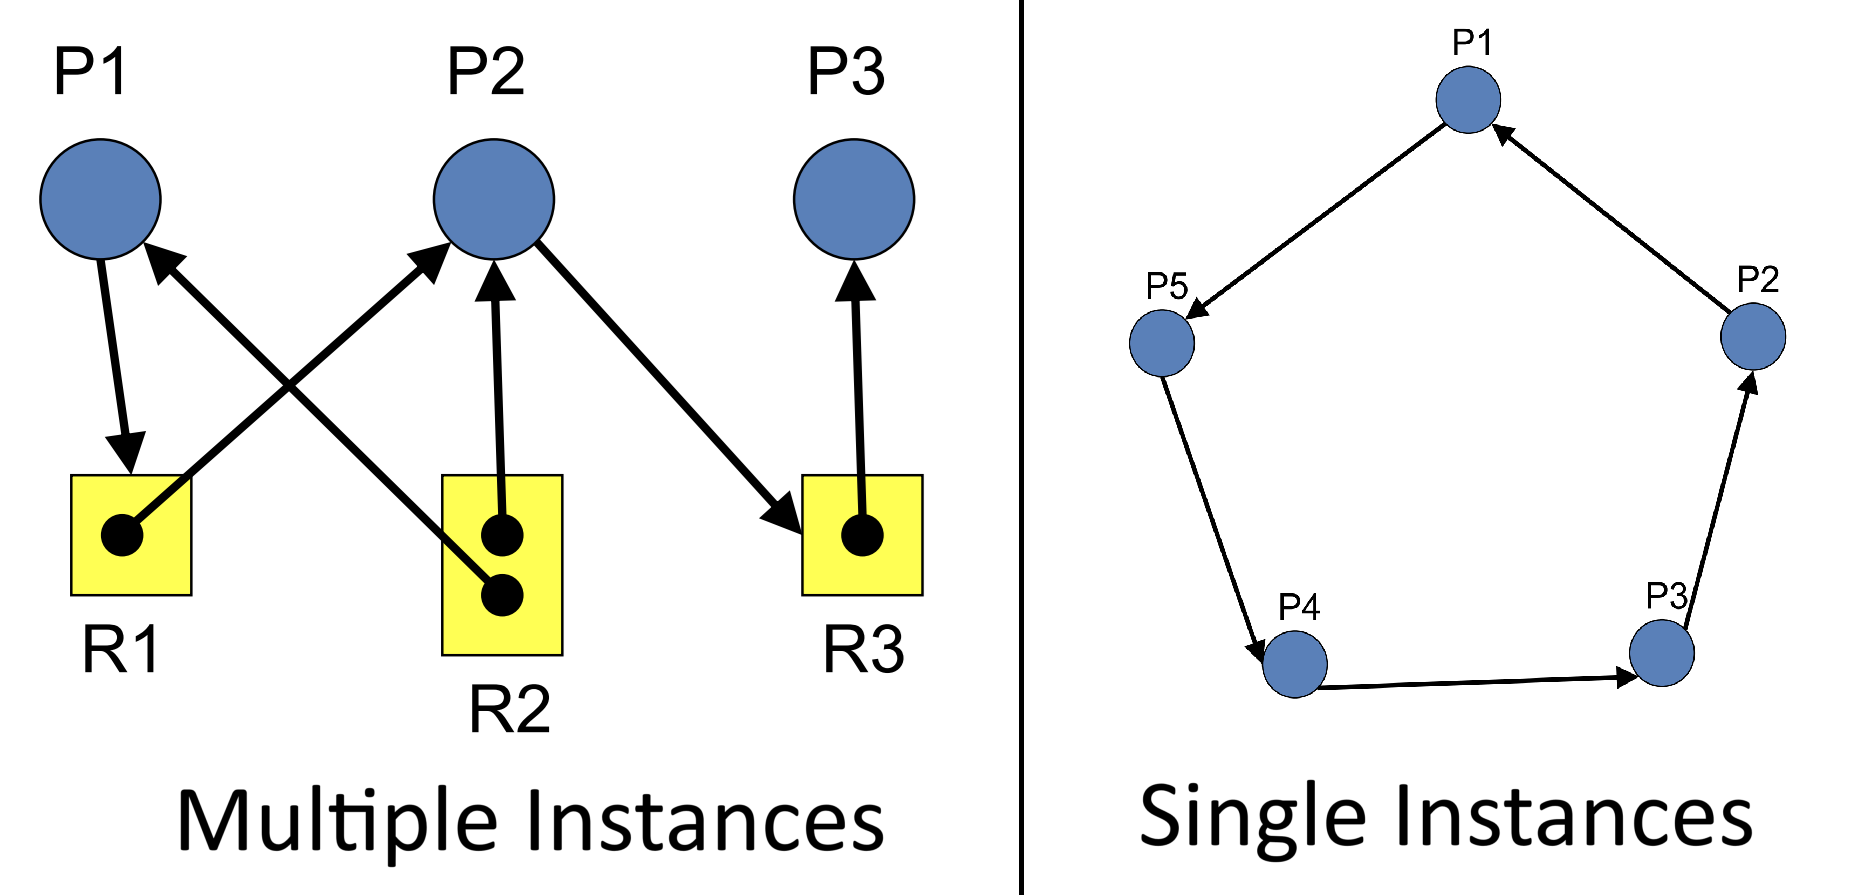
\includegraphics[width=0.6\textwidth]{ResourceGraph.png}
  \caption{Resource Allocation Graph}
  \label{fig:Resource_Allocation_Graph}
\end{figure}


\paragraph{Necessary Conditions for Deadlocks} \red{All} of the following \red{must hold} for a deadlock to occur:
\begin{enumerate}
  \item \textbf{Mutual Exclusion:} \par
        At least one resource must be held in a non-shareable mode, i.e. only one process at a time can use the resource. \gray{if every resource is shareable or used by a single process, then no deadlock can occur.}

  \item \textbf{Hold \& Wait:} \par
        Processes holding resources are allowed to request additional resources without releasing the resources they already hold. \gray{If processes must release all resources before requesting new ones or atommically request all resources, then no deadlock can occur.}

  \item \textbf{Circular Wait:} \par
        There must be a circular chain of two or more processes, each waiting for a resource held by the next process in the chain. i.e. \(P(i)\) wait for resource held by \(P((i+1)\%n)\). \gray{Otherwise there exists at least one process that doesn't need to wait}

  \item \textbf{No Resource Preemption:} \par
        Resources cannot be forcibly taken from a process holding them, they must be voluntarily released. \gray{If resources held can be released after some period of time, then no deadlock can occur.}
\end{enumerate}


\paragraph{Dealing with Deadlocks} There are \textbf{3} main strategies to deal with deadlocks:
\begin{itemize}
  \item \textbf{Deadlock Prevention:} Violate one of the 4 conditions necessary for deadlock to occur.

  \item \textbf{Deadlock Detection \& Recovery:} Allow the system to enter deadlock state, but put in place mechanisms that can detect, and then recover from this situation. Typically refers to killing one or more processes in the deadlock state, using the algorithmic resource-graph problem.

  \item \textbf{Deadlock Avoidance:} Use a resource allocation graph to detect potential deadlocks and avoid them by not allocating resources that would lead to a deadlock. (e.g. Banker's Algorithm). Requires full knowledge of the system's resource requirements and current allocation.
\end{itemize}

\paragraph{Deadlock Prevention} There are 4 conditions for deadlock to occur, and we can prevent deadlocks by violating one of them:
\begin{enumerate}
  \item \textbf{No Mutual Exclusion:} \par
        Making all resources sharable, by implementing some data structure using only hardware-supported atomic operations. These algorithms are called "lock free".

  \item \textbf{No Hold \& Wait:} \par
        Each process must request all resources it needs at once, or release all resources before requesting new ones. The system either grants all resources or none and block the process.
        \textbf{Con:} Processes will hold on to their resources for more time than they actually need them, which limits concurrency and hence limits performance.

  \item \textbf{No Circular Wait:} \gray{the most usable flexible method} \par
        Impose a strict ordering on resources, i.e. number all resources in one sequence. Processes can only request resources in increasing order, a process that wants to acquire a resource that has a lower order must first release all resources it holds that have a higher order.

  \item \textbf{No "No Resource Preemption":} \par
        When needed, choose a victim process and release its resources, allowing other processes to continue. \par
        \gray{e.g. if there isn't enough memory, we can backup the victim's state to disk and release all its memory, or just kill the process.}

\end{enumerate}

\paragraph{Deadlock Detection \& Recovery} If there is \ul{only one instance} of each resource type, then a deadlock can be detected by checking for cycles in the \textbf{simplified resource allocation graph}. In the \ul{general} case \gray{(multiple instances of each resource type)}, Necessary conditions for deadlock are not sufficient, nevertheless, we can still detect deadlocks but it is \textit{outside the scope of this course}. \par

After a deadlock is detected, we can recover from it by: \textbf{(1)} Killing one or more processes in the deadlock state until the deadlock is resolved, or \textbf{(2)} Forcibly preempting resources from one or more processes in the deadlock state. Finding the minimal set of processes to kill/preempt is a hard problem.

In literature, Detection and Recovery refer to the algorithmic problem of finding the minimal set of processes to kill/preempt in the resource graph.

\paragraph{Deadlock Avoidance} The system can avoid deadlocks by not allocating resources that would lead to a deadlock. This is achieved by the \textbf{Banker's Algorithm}, which is a resource allocation and deadlock avoidance algorithm that tests for safety before allocating resources. The algorithm maintains a \textit{safe state} and only allocates resources if it can guarantee that the system will remain in a safe state after the allocation. The algorithm requires knowledge of the maximum resource requirements of each process and the current allocation of resources.

\textbf{Safe State:} A system state where we are sure that all processes can be executed \textbf{in some order}, one after the other, such that each one will obtain all the resources it needs to finish. We assume once a process receives all the resources it needs, it will finish and release all its resources. \par

\paragraph{Rules of the Banker's Algorithm} The Banker's Algorithm works as follows:
\begin{itemize}
  \item There are \(n\) processes and \(k\) resource types \gray{(each resource can have multiple instances)}.
  \item Upon initialization, each process \(p\) \blue{declares the maximal} number of resource-instances it will need for each type, \blue{\(\max[p]\)}.
  \item While running, OS maintains how many resources are \blue{currently allocated} to each process, \blue{\(cur[p]\)}.
  \item And how many resource instances are \blue{currently available (free)}, \blue{\(avail\)}.
  \item Upon a request for resources by a process \(p\), \blue{\(R\)}, the OS allocates iff the system will stay in a safe-state after the allocation. If not, the process is blocked until the resources are available.
\end{itemize}

\textbf{Note:} The Banker's Algorithm is \blue{conservative}, i.e. it will not allocate resources even if there is possibility to allocate them without deadlocking the system. The OS doesn't take chances! With \blue{Time Complexity \(O(n^2)\)}.

\begin{lstlisting}[language=C, caption={Banker's Algorithm}, label={lst:bankers_algorithm}]
// *Assume* that request R was granted to process q
cur[q] += R;                            // vector addition
avail -= R; 
// Check if the system is in a safe state (i.e. all processes can finish in some order)
P = ... // All non-terminated processes (processes that are not finished yet)
while(P is *not* empty){
    found = false                       // true = found a process that can finish
    for each p in P {                   // find a process that can finish
        if (max[p] - cur[p] <= avail) { // can finish? (by maxing its resources)
            avail += cur[p]             // release resources (pretend p finishes)
            P.remove(p)
            found = true
        }
    }
    if (!found) return FAILURE
}
return SUCCESS
\end{lstlisting}




% =====================================================
% =========== Lecture NETWORKING ======================
% =====================================================



\newpage
\Topic{Networking}

\paragraph{Protocol} A protocol is a set of rules defining the \textit{format \& order} of messages sent \& received, and what actions are taken upon message transmission or receipt.


\begin{figure}[H]
  \centering
  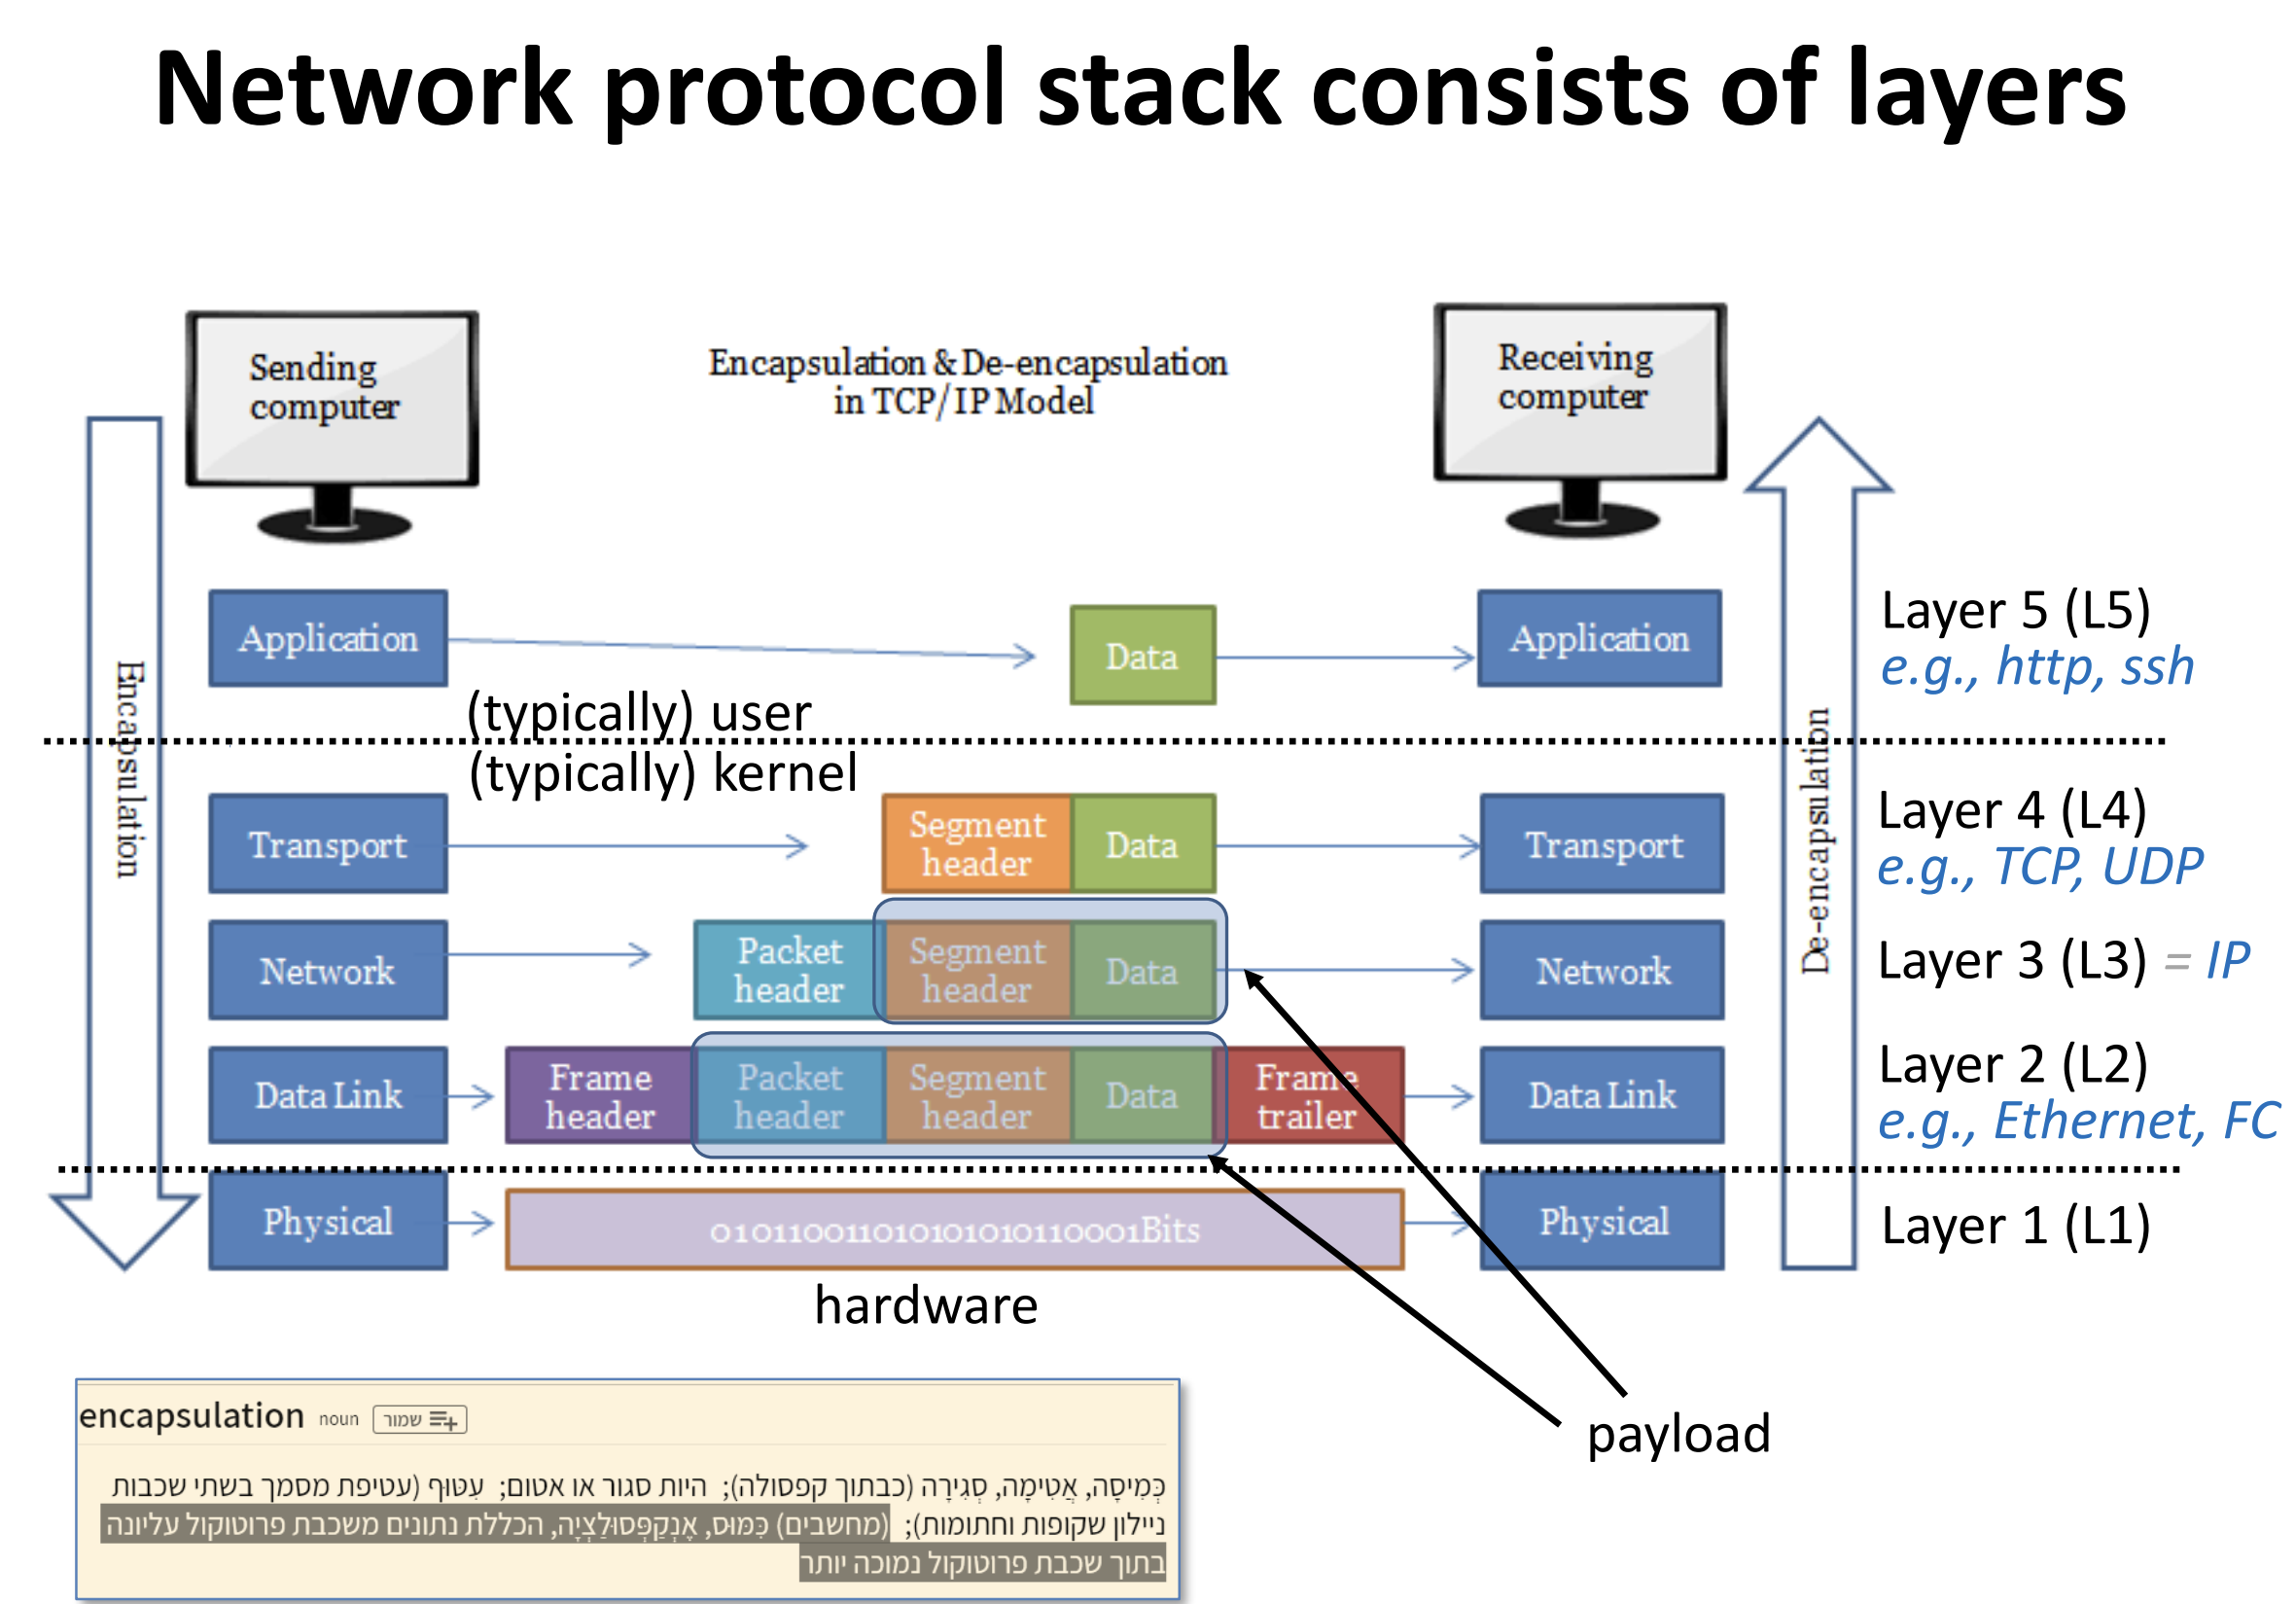
\includegraphics[width=0.8\textwidth]{NetworkLayers.png}
  \caption{Network Layers Overview}
  \label{fig:networking_overview}
\end{figure}

In a nutshell, networks can be divided into 5 layers as follows:
\begin{itemize}
  \item \textbf{Application Layer - L5:} The top layer, where applications communicate with each other. Examples include HTTP, FTP, SMTP, etc.
  \item \textbf{Transport Layer - L4:} Responsible for end-to-end communication between applications. It provides reliable or unreliable delivery of data. Examples include TCP (reliable) and UDP (unreliable).
  \item \textbf{Network Layer - L3:} Responsible for routing data between devices on different networks. It provides logical addressing and routing. Examples include IP (Internet Protocol).
  \item \textbf{Data Link Layer - L2:} Responsible for node-to-node communication within the same network. It provides physical addressing and error detection. Examples include Ethernet, Wi-Fi, etc.
  \item \textbf{Physical Layer - L1:} The lowest layer, responsible for the physical transmission of data over a medium. It includes the hardware components such as cables, switches, and network interface cards (NICs).
\end{itemize}




\begin{table}[H] % Using [H] from the 'float' package to place it here
\centering
\renewcommand{\arraystretch}{1.5} % Increases row height for better spacing

% The \rowcolors command handles the alternating colors automatically and robustly
\rowcolors{2}{white}{tableBlue} 

\begin{tabular}{|c|l|l|l|l|>{\centering\arraybackslash}p{3.5cm}|}
    % The header row still needs its own color specifications
    \rowcolor{tableBlue}
    \textbf{layer} & \textbf{name} & \textbf{protocols} & \textbf{data unit} & \textbf{addressing} & \multicolumn{1}{c|}{\cellcolor{headerRed}\color{white}\textbf{implemented by}} \\
    \hline

    % NOTE: No more \rowcolor commands needed on each line below!
    
    \textbf{5} & application & HTTP, SMTP & stream, messages & N/A & user-level code \\
    \redhline

    \textbf{4} & transport & TCP, UDP & segments, datagrams & ports & \multirow{3}{=}{\centering kernel-level code (the operating system)} \\
    \cline{1-5}

    \textbf{3} & network & IP & packets & IP & \\
    \cline{1-5}

    \textbf{2} & link & ethernet & frames & MAC & \\
    \redhline

    \textbf{1} & physical & 802.11 & bits & N/A & hardware (NIC) \\
    \hline
\end{tabular}
\caption{A five-layer network model describing protocols, data units, and implementation levels.}
\label{tab:network-layers} % It's good practice to add a label for referencing
\end{table}





\noindent\rule{\linewidth}{0.5pt}

\section*{Application Layer (L5)}

The Application Layer is the topmost layer in the network architecture. It provides network services directly to the user's applications. This layer is responsible for facilitating communication between software applications and lower layers of the network stack.

The Application Layer interacts with the Transport Layer (L4) to establish connections and manage data flow between applications on different devices. One can easily invent a new protocol as needed.

There are \textbf{Standard} protocols (determined by multiple organizations): HTTP, HTTPS, NFS, SSH, Bitcoin...
And \textbf{Proprietary} protocols (determined by a single organization): Microsoft Exchange, Skype, Zoom, Whatsapp...

\paragraph{Problems In Networking - } There are 2 main problems to consider when discussing networks:
\begin{itemize}
  \item \textbf{Lossiness:} Networks are inherently lossy, meaning that data sent won't always arrive at the destination. This can be due to various reasons such as hardware failures... But more commonly, it is due to running out of \textit{memory buffer space} in network elements.
  \item \textbf{Reordering:} Networks may mess up the order of the messages sent.
\end{itemize}





\noindent\rule{\linewidth}{0.5pt}


\section*{Transport Layer (L4)}

Protocols in Layer 4 provide host-to-host communication services \textit{for processes}, they are implemented (typically) by the OS. Two most common protocols are: \textbf{TCP} (Transmission Control Protocol) and \textbf{UDP} (User Datagram Protocol).

\paragraph{TCP} "The protocol that cares", i.e. it cares about data loss \& reordering. It ensures that data is delivered reliably and in the correct order. Provides \textbf{stream} of bytes between two processes. Said to be \textbf{connection-oriented} because it establishes a connection before transmitting data. Simplified view of TCP:
\begin{itemize}
  \item \textbf{Sender}
        \begin{enumerate}
          \item Establish a connection with the receiver by performing a \textit{3-way handshake}.
          \item Split bytes into contiguous chunks called \textit{segments}.
          \item Assign a sequence number to each segment, and keep them around until they are acknowledged by the receiver.
          \item Resend segments that are not acknowledged for some time, or receiver says they are missing.
          \item Slow down the sending rate if segments sent are not reaching the receiver.
          \item Implement \textbf{Congestion Control} = changing the rate in response to drops.
        \end{enumerate}
  \item \textbf{Receiver}
        \begin{enumerate}
          \item Send ack messages (acknowledgments) upon receiving chunks.
          \item Ask sender to resend chunks that appear to be missing for some time.
          \item "Advertise" free buffer space to the sender, so it knows how much data it can send without overflowing the receiver's buffer.
          \item Implement \textbf{Flow Control} (advertising) = Receiver controls sender transmission rate, thereby preventing its own buffer overflow.
          \item Deliver the bytes in-order to receiving user-level app.
        \end{enumerate}
\end{itemize}


\paragraph{TCP Sequence Numbers} TCP uses sequence numbers to ensure that data is delivered in the correct order. Each byte in the stream is assigned a unique sequence number, and the receiver uses these numbers to reassemble the data in the correct order. The sequence number is included in each segment header, allowing the receiver to detect missing segments and request retransmission. 

For each segment sent, the sender waits for an acknowledgment message from the receiver, if he doesn't receive any (the original message or the acknowledgment were lost) he resends the same segment with the same number. The receiver checks the number to prevent multiplicity in case of lost acknowledgment messages.

\paragraph{UDP} "The protocol that doesn't care", i.e. it \red{does not} guarantee reliable delivery nor in-order delivery of data. Provides \textbf{datagrams} (as opposed to a stream) of bytes between two processes. Chunks might get lost or be delivered out of order, \red{but} per-chunk bytes integrity is supported. Said to be \textbf{connectionless} because it does not establish a connection before transmitting data. Compared to TCP, UDP is simpler and has less overhead, lower latency, and no congestion control.

Note: To clarify, UDP still offers some level of reliability, as it uses \textit{checksums} CRC error detection to ensure that the data received is not corrupted. However, it does not guarantee that the data will be delivered or that it will be delivered in the correct order.

\paragraph{Sockets} Apps communicate with the Transport Layer through \textbf{socket file descriptors}, created via the \code{socket()} system call, instead of \code{open()}. A \textbf{\code{sockfd}} constitutes a communication endpoint.

Note: It is recommended to understand what IPs are before continuing this section (\gray{read next section - IP})

\paragraph{Ports} Ports exist on the same host, and there can be a multiple of them. Each communicating process utilizes \code{sockfd}s to identify its own communication channel, each with its own associated \textbf{port}. As IPs are not sufficient, we use a unique port for each socket, which is an \blue{unsigned 16-bit integer} that identifies it on the host. Each chunk transmitted is associated with IP-address + port.


Ports can either be \textbf{Ephemeral} (temporary, dynamically assigned by the kernel), or \textbf{Well-Known} (static, determined by standards/known values). \red{Ports \(\leq\) 1023} are reserved for well-known protocols, such as HTTP (80), HTTPS (443), etc.

Each socket is identified by a \textbf{5-tuple} consisting of: \\
1. Source IP address \\
2. Source port number \\
3. Destination IP address \\
4. Destination port number \\
5. Transport protocol (e.g. TCP, UDP)


\subsection*{Client-Server Model (TCP)}
In the client-server model, a server listens for incoming connections from clients, and clients initiate connections to the server. The \textbf{server} \blue{passively} waits for client requests and then reacts, "request-response" paradigm. The server has a well-known domain name (and/or IP address) \& port. The \textbf{client} asynchronously/intermittently connects to the server, sends requests, and waits for responses. The client may have dynamic IP, and may use ephemeral port.

Sockets are initialized using values from \code{addrinfo} structure, which contains the following info: (1) Protocol family (e.g. IPv4, IPv6), (2) Protocol type (TCP), (3) Socket type (stream), (4) server/client.


% --- Table code begins ---
\begin{samepage}
  \begin{center}
    \textbf{Creating and Using TCP Sockets}
    \rowcolors{2}{gray!15}{white}
    \begin{tabular}{|>{\raggedright\arraybackslash\ttfamily}p{4cm}|
                     >{\centering\arraybackslash}p{5.5cm}|
                     >{\raggedright\arraybackslash\ttfamily}p{4cm}|}
      \hline
      \rowcolor{blue!50}
      \textcolor{white}{\textbf{server}} &
      \textcolor{white}{\textbf{message}} &
      \textcolor{white}{\textbf{client}} \\
      \hline
      srvfd = socket(...) & & sockfd = socket(...) \\
      
      bind( srvfd , port ) & & \\
      
      listen( srvfd ) & & \\
      
      \normalfont\textit{loop:} & & \\
      
      clifd = accept( srvfd ) &
      \red{$\xleftarrow{\text{\textcolor{black}{request service (transport)}}}$ } &
      connect( sockfd , host+port ) \\
      
      read(clifd ) &
      \red{$\xleftarrow{\text{\textcolor{black}{request (application)}}}$ } &
      write( sockfd ) \\
      
      write( clifd ) &
      \red{$\xrightarrow{\text{\textcolor{black}{response (application)}}}$ } &
      read( sockfd ) \\
      \hline
    \end{tabular}
  \end{center}
\end{samepage}
% --- Table code ends ---



\paragraph{Event Oriented Programming - \code{select()}} In the client-server model, the server can handle multiple clients simultaneously by using the \code{select()} system call. This allows the server to monitor multiple sockets for incoming data and handle them as they arrive, without blocking on any single specific socket (we block on them all together until one is available). The server can use \code{select()} to wait for data on multiple sockets, and when data is available, it can read from the corresponding socket and respond accordingly.

\begin{lstlisting}[language=C]
int select(int nfds, fd_set *readfds, fd_set *writefds, fd_set *errorfds, struct timeval *restrict timeout);
\end{lstlisting}

\begin{itemize}
  \item nfds: The highest-numbered file descriptor in any of the three sets, plus one.
  \item readfds: A set of file descriptors to be monitored for reading.
  \item writefds: A set of file descriptors to be monitored for writing.
  \item errorfds: Not part of the course material.
  \item timeout: A pointer to a \code{timeval} structure that specifies the maximum time to wait for an event. If \code{NULL}, it will block indefinitely until an event occurs.
\end{itemize}






\noindent\rule{\linewidth}{0.5pt}



\section*{Network Layer (L3) - IP}

The Network Layer is responsible for routing data between devices on different networks. It provides logical addressing and routing. The most common protocol in this layer is the Internet Protocol (IP).

\paragraph{Domain \& Host Names} Computers are associated with hierarchical human-readable "domain" names, sometimes referred to as host names, e.g. \textit{www.google.com}. Each domain names can be backed by one or more host machines, but we will use the term host name assuming it corresponds to a single host machine.


\paragraph{IP Address} Domain names are only for humans to read, but computers need to know the \textbf{IP address} of the host they want to communicate with. An IP address is a unique identifier assigned to each device connected to a network. Each host is mapped to a 32-bit IP address obtained via a domain name resolution protocol called \textbf{DNS} (Domain Name System). \gray{"IP" for us stands for IPv4 (Internet Protocol version 4), but there is also IPv6 which is a 128-bit address space which we will ignore.}

Each IP address corresponds to a single host, unlike domain names. Domain names can point to multiple IP addresses (e.g. load balancing), while each IP address is unique to a specific host. The opposite is also not true, i.e. one host can have multiple IP addresses. For simplicity we will assume there's a 1-to-1 host-to-IP mapping.

Note: IP is used to identify host machines, while ports are used to identify individual communication channels of processes on the host.



% --- Start of the example ---
\vspace{0.5em} % Adds a little vertical space before the table
\begin{center}
  For example, the IP of \texttt{csa.cs.technion.ac.il} is
  \begin{tabular}{ll}
    \toprule
    \textbf{Notation}      & \textbf{IP address}                                                              \\
    \midrule
    Decimal                & 2219057153 \textcolor{gray}{(not terribly convenient)}                           \\[1.5ex]
    Binary (8x4 = 32 bits) &
    $\overset{132}{\texttt{10000100}} \enspace | \enspace
      \overset{68}{\texttt{01000100}} \enspace | \enspace
      \overset{32}{\texttt{00100000}} \enspace | \enspace
    \overset{1}{\texttt{00000001}}$                                                                           \\[1.5ex]
    Dot-decimal            & \textcolor{blue!80!black}{132.68.32.1} \textcolor{gray}{(a bit more convenient)} \\
    \bottomrule
  \end{tabular}
\end{center}
% --- End of the LaTeX code for the table ---



\noindent\rule{\linewidth}{0.5pt}


\section*{Physical-Layer (L1) \& Link Layer (L2)}

\paragraph{LAN (Local Area Network)} A LAN is a network that connects devices within a limited geographical area, such as a home, office, or campus. It typically uses Ethernet or Wi-Fi technologies to connect devices. Each LAN device is equipped with \textbf{Network Interface Card (NIC)}, which is a hardware component that allows the device to connect to the network. 

We will focus on Ethernet, which is the most common LAN technology. 

\paragraph{Ethernet} Ethernet is a protocol that combines hardware, firmware, and software (OS). Ethernet is both a link-layer protocol (L2) as it allows nodes to communicate within the LAN by sending \textbf{frames} (byte chunks in layer L2), and a physical-layer protocol (L1) as it defines raw bits are transmitted over the physical medium.

\paragraph{MAC (Media Access Control) Address} Each device on a LAN has a unique identifier called a \textbf{MAC address}. It is a 48-bit address that is assigned to the NIC by the manufacturer. The MAC address is used to identify devices on the same LAN and is used by Ethernet to deliver frames to the correct destination. The 48-bits are usually represented as 6 hexadecimal numbers separated by colons, e.g. \texttt{00:1A:2B:3C:4D:5E}, where the first 3 bytes are the device's manufacturer ID and the last 3 bytes are the device's unique identifier.




\paragraph{Ethernet Frame Structure} An Ethernet frame is the basic unit of data transmission in Ethernet networks. It consists of several fields that provide information about the frame and its contents. The structure of an Ethernet frame is as follows:

\begin{figure}[H]
\centering
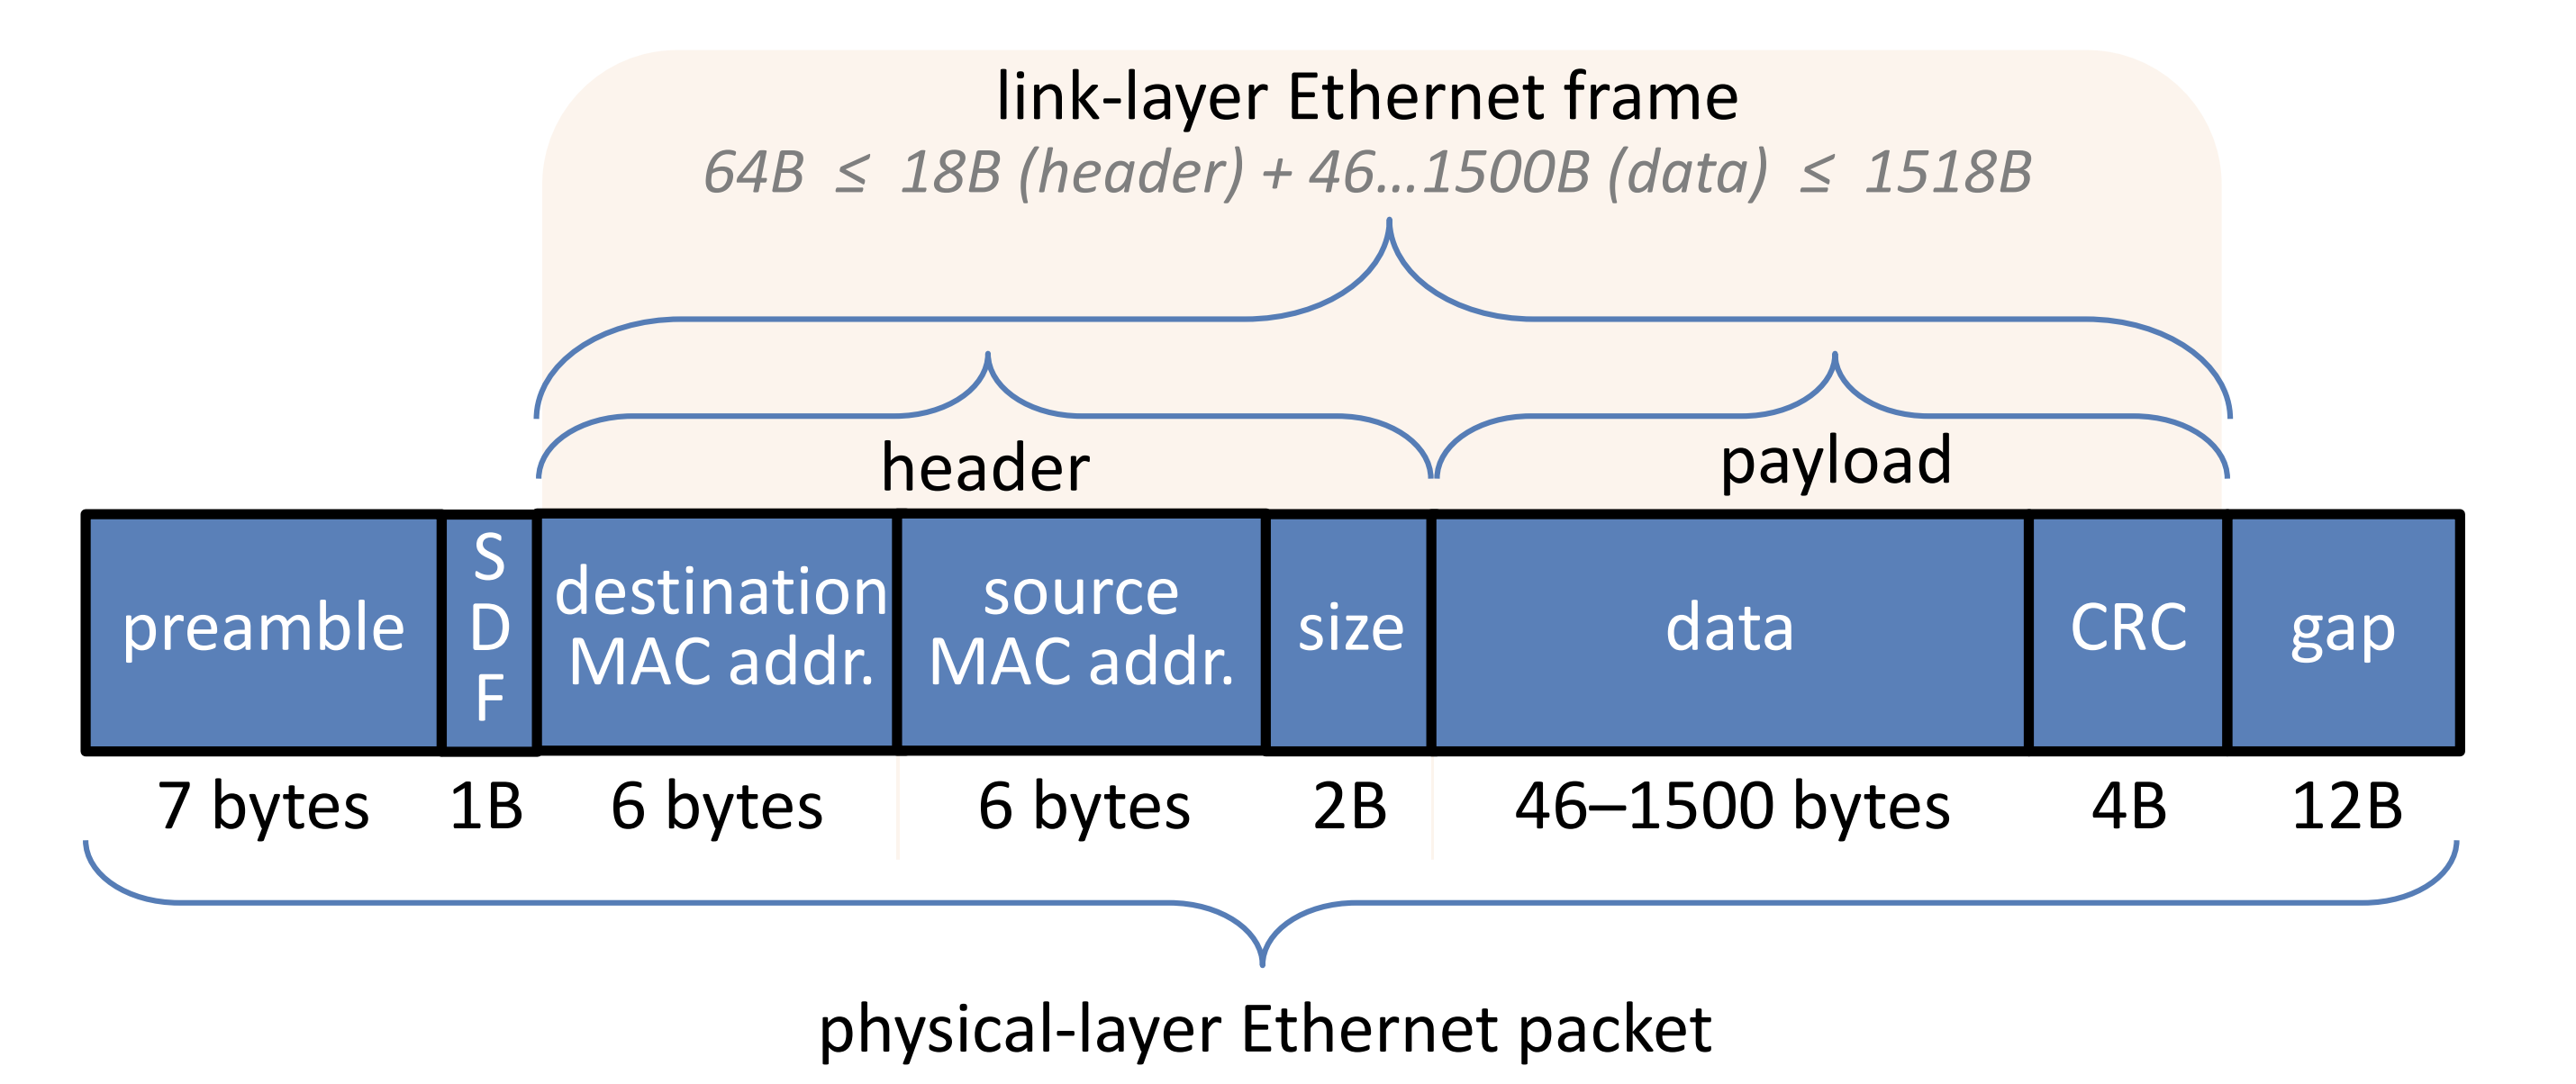
\includegraphics[width=0.7\textwidth]{EthernetFrame.png}
\caption{Diagram of an Ethernet Frame Structure.}
\end{figure}

\begin{enumerate}
    \item \textbf{Preamble:} Its purpose is purely for timing and synchronization. 

    \item \textbf{Start Frame Delimiter (SFD):} The actual frame starts with the very next bit.

    \item \textbf{Destination/Source MAC Address:}
    This is the MAC of the NIC that the frame is \textit{intended for} (Destination) and the MAC of the NIC that \textit{sent} the frame (Source).

    \item \textbf{Size:} Represents the length of the frame.

    \item \textbf{data:} Contains the actual data from the upper layers, such as an IP packet from the Network Layer (L3).

    \item \textbf{Cyclic Redundancy Check (CRC):} It is an \red{error-detection code}. i.e. the frame is dropped in case of a CRC error.

    \item \textbf{Gap:} After a frame is sent, devices on the network must wait for a brief period before any device is allowed to send the next frame. This gives device interfaces time to process the frame they just received and prepare for the next one.
\end{enumerate}


\noindent\rule{\linewidth}{0.5pt}


\section*{The Internet}

\paragraph{IP \& Routers} The problem for now is LAN hardware communicate through L2, meaning two different LANs cannot communicate with each other. The solution is to use \textbf{routers}, which are devices that connect different networks and \textbf{forward} packets between them. Thus the internet is a inter-network of networks, where each inter-network is connected by routers. This is made possible using the IP (L3) protocol, which provides a way to route packets between different networks. The routers "peel off" the L2 headers of the source LAN and re-encapsulate the data within L2-headers of the destination LAN.  

\begin{figure}[H]
    \centering
    \begin{subfigure}[b]{0.5\textwidth}
        \centering
        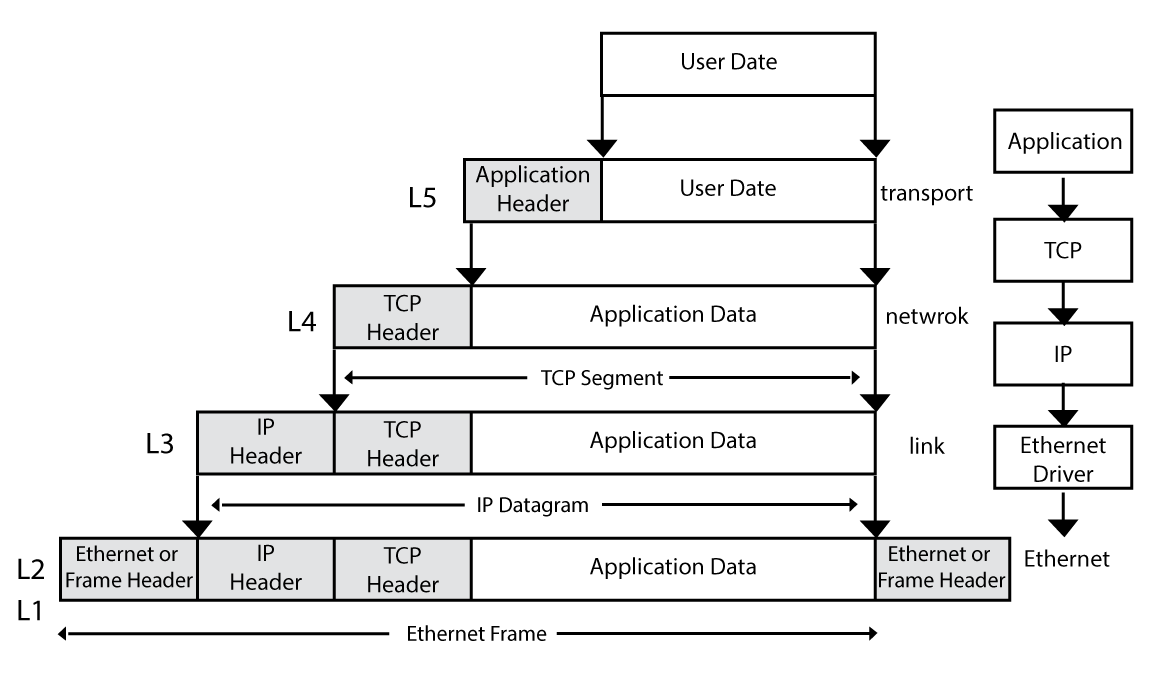
\includegraphics[width=\textwidth]{network-layers.png}
        \caption{The Internet Layers and Encapsulation.}
        \label{fig:network-layers}
    \end{subfigure}
    \hfill % This creates a horizontal space between the images
    \begin{subfigure}[b]{0.4\textwidth}
        \centering
        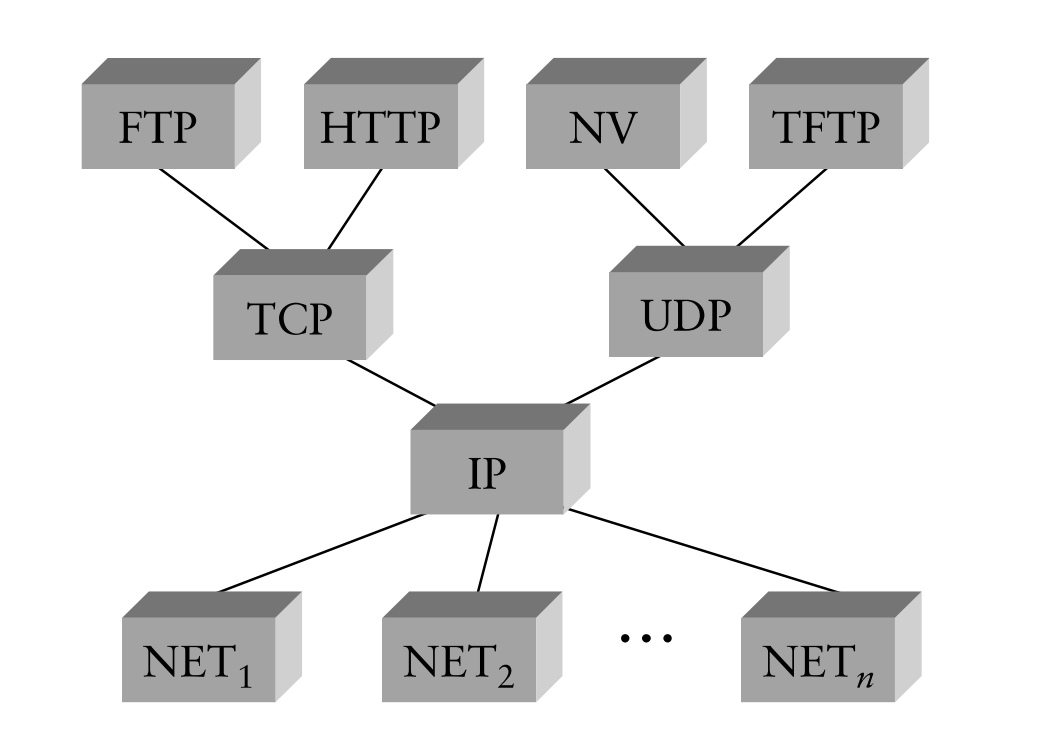
\includegraphics[width=\textwidth]{hourglass.png}
        \caption{Hourglass Model of the Internet.}
        \label{fig:hourglass}
    \end{subfigure}
\end{figure}

\paragraph{Hourglass Model} The hourglass model is a conceptual framework that illustrates how the Internet is structured. It shows that the Internet has a narrow waist, which is the IP protocol, and that all other protocols (e.g. TCP, UDP, HTTP) are built on top of it. The model emphasizes the importance of IP as the foundation of the Internet, allowing different protocols to coexist and communicate with each other.



\paragraph{IP address structure} An IP consists of two parts: \textbf{\blue{Subnet} Part} (high order bits) and \textbf{\blue{Host} Part} (low order bits). The subnet part identifies the network, while the host part identifies the specific device within that network. The subnet part is determined by the \textbf{subnet mask}, which is a 32-bit number that specifies how many bits are used for the subnet part and how many bits are used for the host part. An IP address is \red{always} coupled with a subnet mask; e.g. \code{192.168.1.1/24} means that the first 24 bits are the subnet part and the last 8 bits are the host part. \textbf{Meaning of subnet} is that all devices in the same subnet can communicate with each other directly, without going through a router. i.e. it defines the boundaries of the Ethernet LAN.


\paragraph{ARP (Address Resolution Protocol):} \blue{IP \(\Longrightarrow\) MAC} \\
ARP is a protocol used to map IP addresses to MAC addresses. When a device wants to communicate with another device on the same local network, it needs to know the MAC address of the destination device. If it only knows the IP address, it \blue{broadcasts} an ARP query packet (containing the destination IP and -1 as the MAC) to the local network, asking "Who has IP address X.X.X.X? Tell me your MAC address." The device with the matching IP address responds with its MAC address, allowing the sender to encapsulate the data in a frame and send it to the correct destination. If the destination is not on the same local network, the sender will get the MAC to \textbf{its default gateway (router)}, its first-hop router, which will then forward the packet to the correct destination network.

\paragraph{NAT (Network Address Translation):} \gray{private IPs} \\
NAT is a technique used to allow multiple devices on a local network to share a single public IP address. NAT defines new private IP addresses for each device on the local network, allowing them to communicate with each other using these private addresses. When a device wants to communicate with the outside world, NAT translates its private IP address to the public IP address, allowing the device to access the internet. This helps conserve the limited pool of public IP addresses and provides an additional layer of security by hiding the internal network structure from external entities. To do so, NAT maintains a mapping between pairs of (private IP addresses + port) and (public IP address + port).


\paragraph{DHCP (Dynamic Host Configuration Protocol):} \blue{get an IP} \\
DHCP is an \red{L5 protocol} used to dynamically assign IP addresses to devices on a network. The goal of DHCP server is to \blue{allow client's host to dynamically get IP address when joining LAN}, which can provide: \ul{(1) subnet mask, (2) Default gateway (first hop router), (3) Name + IP of DNS server for client}. DHCP uses \textbf{UDP} to communicate allowing the ability to broadcast to all hosts in LAN. When a device connects to a network, it sends a DHCP request to the DHCP server, which responds with an available IP address and other configuration information. 






% =====================================================
% =========== Lecture Virtual Memory ==================
% =====================================================



\newpage
\Topic{Virtual Memory}

\red{NOTE:} ALWAYS say if you are talking about \textbf{physical memory} (RAM) or \textbf{virtual memory} in your answers.

\section*{Virtual Memory Concepts}

\paragraph{Virtual Memory} Virtual memory is the abstraction of physical memory, allowing processes to "think" they have access to the entire memory space, even if the physical memory is limited. The motivation for virtual memory (vmem): 
\begin{itemize}
  \item \textbf{Per-Program Contiguous Memory Illusion:} Each process has its own virtual address space, which is contiguous simplifying memory management and allowing processes to use the same address space without conflicts.
  
  \item \textbf{Isolation:} Virtual memory provides isolation between processes, ensuring that one process cannot access the memory space of another process. 
  
  \item \textbf{Dynamic Growth:} Virtual memory allows processes to grow their heap/stack (and \code{mmap} regions) as needed.
  
  \item \textbf{Illusion of Large Memory:} Virtual memory allows processes to use more memory than is physically available. Allowing for memory \blue{overcommitment}. 
  
  \item \textbf{Access Control} Deciding if individual memory chunks (pages) can be read/written/executed.
\end{itemize}


\paragraph{Fragmentation} Virtual memory also solves the problems of fragmentation: (1) External fragmentation - wasting external chunks of data due to lack of contiguity, caused by spreaded allocations and deallocations, (2) Internal fragmentation - wasting internal chunks of data within allocated pages, due to allocating too much memory for a process, which is not used.


\paragraph{Terminology} \textbf{Virtual Address (VA)} is the address used by a process (\& programmer) to access its own memory space, the CPU processes VAs. \textbf{Physical Address (PA)} is the actual address in RAM where data is stored. \textbf{Page} = chunk of contiguous data (in virutal or physical space), \textbf{Frame} = physical memory exactly big enough to hold one page. \blue{\(|\text{Page}|=|\text{Frame}|=2^k\)}, typically \blue{4KB (k=12)}.


\paragraph{The basic idea} The OS maps virtual addresses to physical addresses using a \textbf{page table}, such that VA spaces are contiguous. Pages can be mapped to: (1) memory, (2) disk, (3) unallocated yet \gray(allocated on-demand).all programs are written using VAs, OS sets the VA\(\Longrightarrow\)PA mapping (governs control plane), HW does on-the-fly translation from VA to PA (governs data plane). 


\begin{figure}[h!]
  \centering
  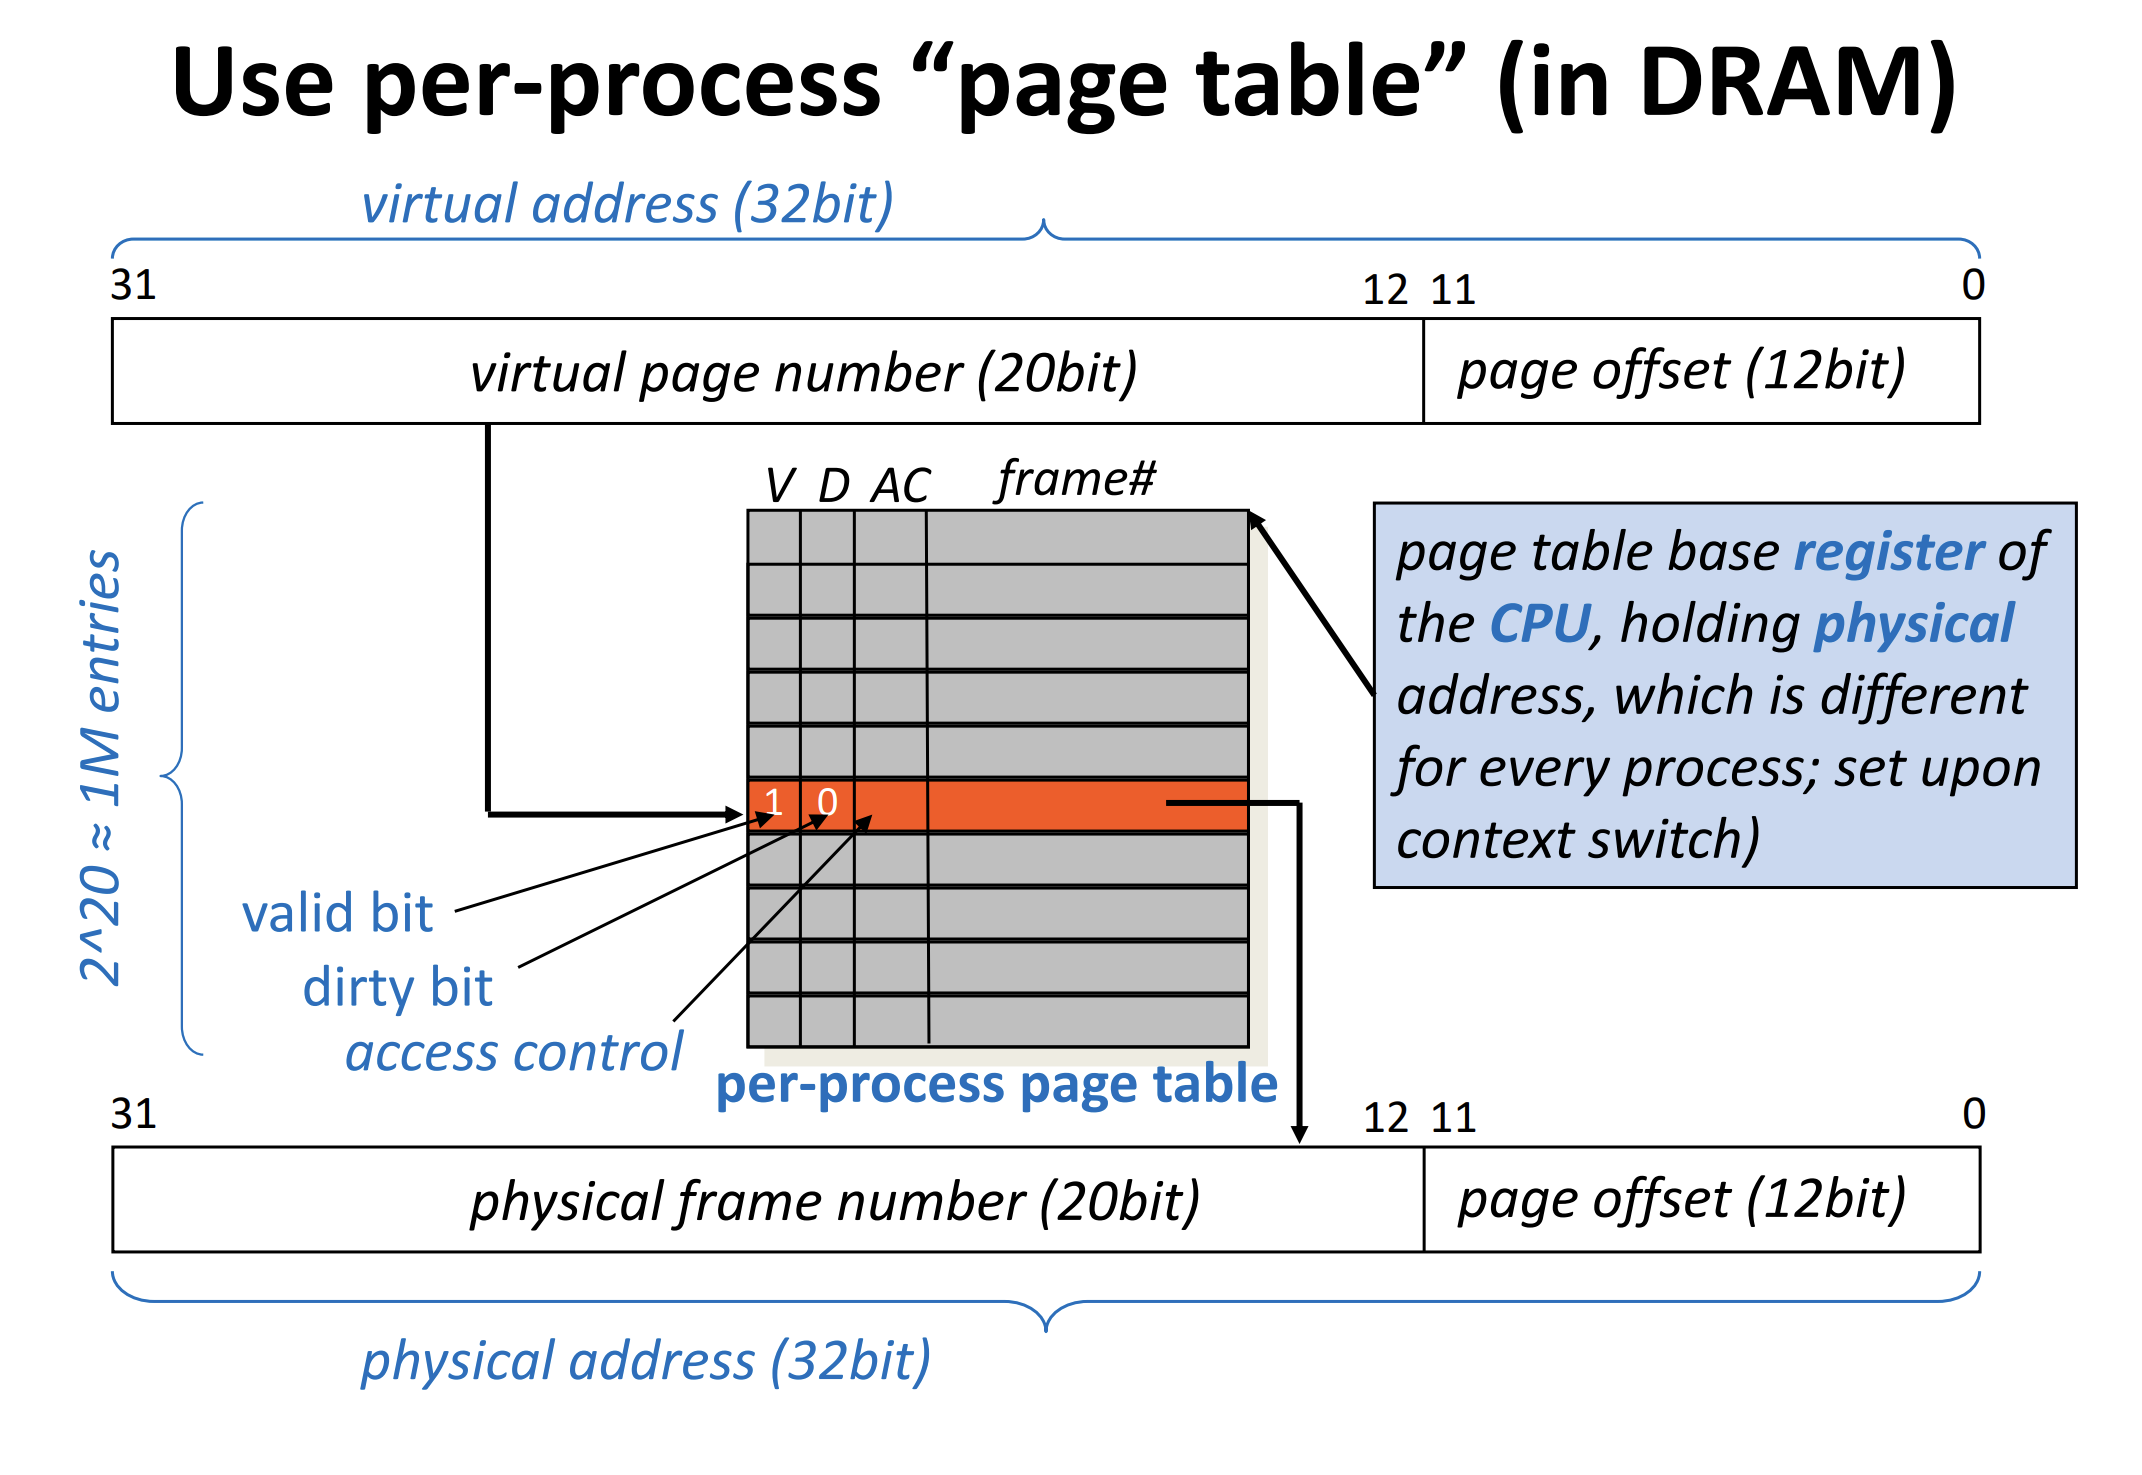
\includegraphics[width=0.6\textwidth]{page-table.png}
  \caption{Virtual Memory Page Table}
\end{figure}


The basic premise of \textbf{page tables} is that each process has its own page table, which maps virtual pages to physical frames. Using the virtual page number (VPN) we check the page table entry \blue{(PTE)} associated with it to find the physical frame number (PFN) it is mapped to, in addition to other flags. One important flag is the \textbf{valid bit}, which indicates whether the page is currently mapped to a physical frame or not. If the valid bit is set, the page is mapped to a physical frame, and the OS can access it. If the valid bit is not set, then if all other bits are zero it means the page has \red{not} been allocated yet. Otherwise it means it resides on the disk in the written address. 



\paragraph{Memory Access steps} the following is the basis of how the CPU accesses memory:
\begin{lstlisting}[language=C, caption={Memory Access Steps in Virtual Memory}, label={lst:memory_access}]
if (valid == 1)                       // Otherwise HW raises a page fault interrupt
    page is in main memory @ PA stored in table \(\Longrightarrow\) data can be used
else if (page resides on disk)        // "Major" page fault
    OS suspends process
    Fetches page from disk and adds VA\(\Longrightarrow\)PA mapping to page table
    Resumes process, which will re-execute faulting instruction
else if (should be but still is not allocated ||
         in page cache but not in page table) // "Minor" page fault
    OS allocates page if needed & adds VA\(\Longrightarrow\)PA mapping to page table
else if (some other legal situations for which OS is responsible)
    Resolve (example: CoW; see later)
else                          // process performed an illegal memory ref
    OS (which handles the page fault interrupts) delivers a signal
    (SIGSEGV/SIGBUS) to the offending process
    The matching signal handler terminates process by default
\end{lstlisting}

If access type is incompatible with specified access rights, then a protection violation fault happens raising an interrupt, which the OS resolves if it is its fault, or delivers a signal to the offending process.


\paragraph{Major Page Fault Flow} Major = need to fetch page from disk.
\begin{enumerate}
  \item \textbf{CPU detects} the situation (valid bit = 0)
  \item \textbf{CPU generates interrupt} and transfers control to the OS
  \item \textbf{OS regains control}, realizes page is on drive, initiates I/O read ops
  \item \textbf{OS suspends the process} \& context switches to another process
  \item \textbf{Upon read completion}, OS makes the process runnable again
  \item When the \textbf{process is scheduled} again, it \ul{re-executes the faulting instruction (which will succeed this time)}
\end{enumerate}


\paragraph{Minor Page Fault} Minor = NO need to go to drive to resolve.
Examples: (1) \textbf{CoW (Copy on Write)} which is used to implement fork for example, (2) \textbf{Demand-based (Lazy) memory allocation}, (3) reading a file content that already is found in the \textbf{page cache}, possibly by other processes.

Note: Minor page faults may cause access to disk if there is not enough memory on DRAM (will cause swapping).

\paragraph{Page in \& out} a chunk of data: \textbf{Paging} is the process of swapping pages in and out of physical memory to disk storage.
$$
\text{Page in} \Longleftrightarrow \text{Copy page from disk to DRAM (read)}
$$
$$
\text{Page out} \Longleftrightarrow \text{Copy page from DRAM to disk (write)}
$$


\paragraph{mmap syscall} The \code{mmap} syscall is used in one of two ways: (1) map a given file to a given virtual address range in the process's memory space. (2) allocate a new \gray{annonymous} memory region in the process's memory space. 
\begin{enumerate}
  \item \textbf{Named Pages:} When mapping a file, the OS maps the file's as if it was an "array of bytes" (backed by the disk) in the VA space of the process. Reads/writes to the mapped region will read/write the file's content, and the OS will update the file accordingly every few seconds, in batches. To force the OS to write the changes to disk, the process can use \code{fsync(fd)} syscall. This helps making programming easier, and saves on the overhead of syscalls to \code{read}/\code{write} \gray(as reads/writes to the \code{mmap} are equivalent to memory reading/writing), which in turn saves on I/O copying.

  \item \textbf{Anonymous Pages:} are heap/stack pages, or pages of \code{mmap} with \blue{\code{fd=-1}, \code{flag=MAP\_ANONYMOUS}} which are \red{not} backed by any file/disk. i.e. we can implement \code{malloc} using \code{mmap} \gray{(for heap we use} \blue{sbrk} \gray{syscall)}.
\end{enumerate}
We also divide the \code{mmap} pages into two types: (1) \textbf{MAP\_SHARED} = changes affect the actual file (\& visible to other processes), (2) \textbf{MAP\_PRIVATE} = changes don't affect the actual fiile; rather, there will be a CoW for the process (other processes will not see changes)

\paragraph{Swapping} \textbf{Swap Space} is a disk area where \red{anonymous} pages are written, if the OS decided they have no room in DRAM (memory is full). Pages are said to be "swapped out" when this occurs (and "swapped in" on return). Nowadays we don't distinguish between the terms swapping and paging.
  

\textit{NOTE:} Kernel memory \red{never swaps out}, it is always in DRAM, and it is not paged in/out. 

Exceptions (for page faults) are divided to: (1) illegal access rights, (2) user access to kernel memory, (3) access to address that is not mapped to any page. The kernel decides the exception using bits for each one and the CPU loads the virtual address to register CR2 (not to be confused with CR3).

\paragraph{On-demand Paging} A memory management technique where pages are loaded into memory only when they are needed, rather than preloading all pages at once. i.e. pages are allocated/brought into DRAM only when the process attempts to access it for the first time (resulting in a page fault)

The steps are: (1) Update the memory region list, (2) Set the page table entry (PTE) present bit as 0, (3) The page is allocated/copies from disk upon first access.

\paragraph{Readahead Prefetching} When \code{read()} identifies sequential accesses to file, the \code{read()} reads ahead pages not yet requested, prefetching them, so they would be ready, in an attempt to minimize page faults. (same with the on-demand paging page fault handler)


\paragraph{Deduplication} A technique to save on physical memory by allocating a single shared page for all processes who use the same data as \textit{read only}.



\paragraph{TLB (Translation Lookaside Buffer)} The TLB is a cache used by the CPU to reduce the time taken to access memory locations. It stores recent translations of virtual memory addresses to physical memory addresses, allowing the CPU to quickly find the physical address corresponding to a virtual address without having to go through the entire page table. When a virtual address is accessed, the CPU first checks the TLB; if the translation is found (a TLB hit), the physical address is retrieved quickly. If not (a TLB miss), the CPU must consult the page table, which is slower. TLBs are typically small and fast, and they use various replacement policies to manage the limited space. 

Typically, HW fills TLB automatically by reading the page table on its own (without SW help), and OS invalidates TLB entries (upon context switches, for non-global entries).





\noindent\rule{\linewidth}{0.4pt}


\section*{Virtual Memory Implementation}

\subsection*{Intel x86 Architecture}

\paragraph{32-bit x86 address translations} 32-bit address means \(2^{32}\) virtual addresses, which is \blue{4GB} of virtual memory space. The virtual address space is divided into pages, typically \(4KB\) in size. The page table maps these virtual pages to physical frames in memory.

\vspace*{0.5em} 

The job of the x86 virtual memory subsystem is to translate 20-bits (=virtual page number - VPN) to 20-bits (= physical frame - PFN). Every process holds a \textbf{Page Directory} (= 4KB page) holding 1024 PDEs (page directory entries) each containing a pointer to a \textbf{Page Table} (= 4KB page) holding 1024 PTEs (page table entries) each containing a point to a \textbf{Page Frame} (= 4KB page). The offset is the last 12 bits of the virtual address, which is used (as is) to access the data in the page frame (same offset). This structure is called \blue{Radix Trees}.

\vspace*{0.5em} 

Each PDE/PTE holds additional flags, such as \textbf{P}resent, \textbf{A}ccessed, \textbf{D}irty, \textbf{U}ser, \textbf{W}riteable, Cache \textbf{D}isabled, etc. 

\paragraph{CR3 Register} The CR3 register holds the \red{physical address} of the page directory for the currently running process. When a context switch occurs, the operating system updates the CR3 register to point to the new process's page directory. (Or more generally, the CR3 register holds the physical address of the first layer of page tables).


\begin{figure}[H]
    \centering
    \begin{subfigure}[b]{0.6\textwidth}
        \centering
        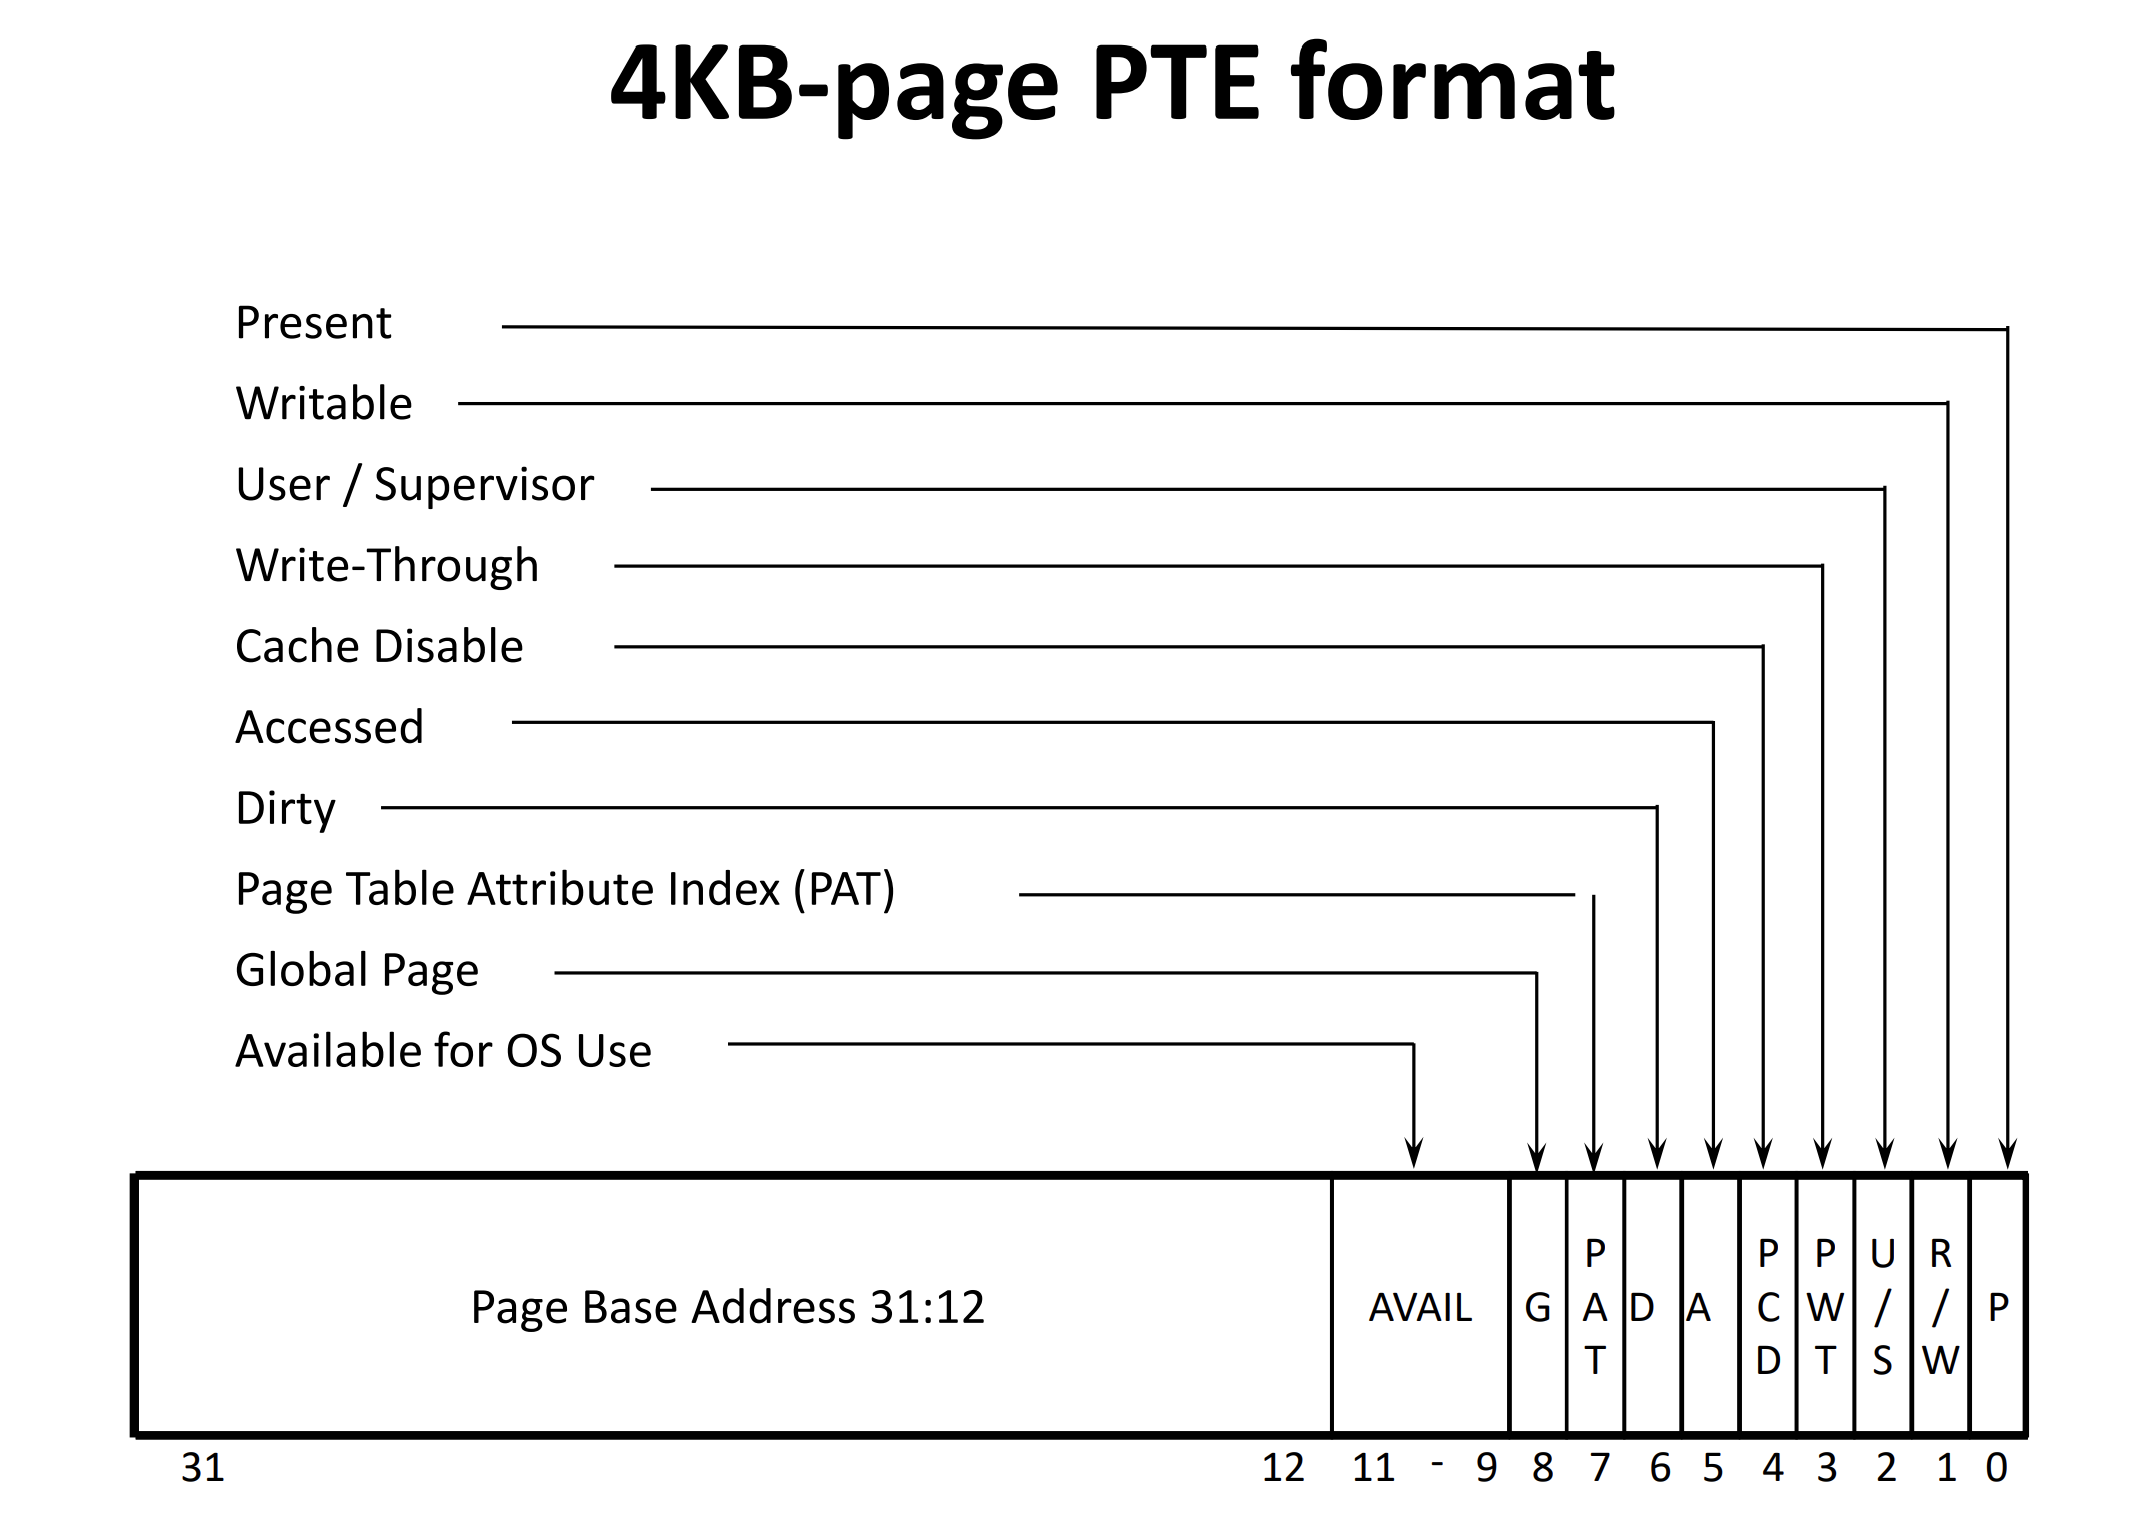
\includegraphics[width=\textwidth]{PTE-format.png}
        \caption{Page Table Entry Format for x86.}
        \label{fig:PTE-format}
    \end{subfigure}
    \hfill % This creates a horizontal space between the images
    \begin{subfigure}[b]{0.3\textwidth}
        \centering
        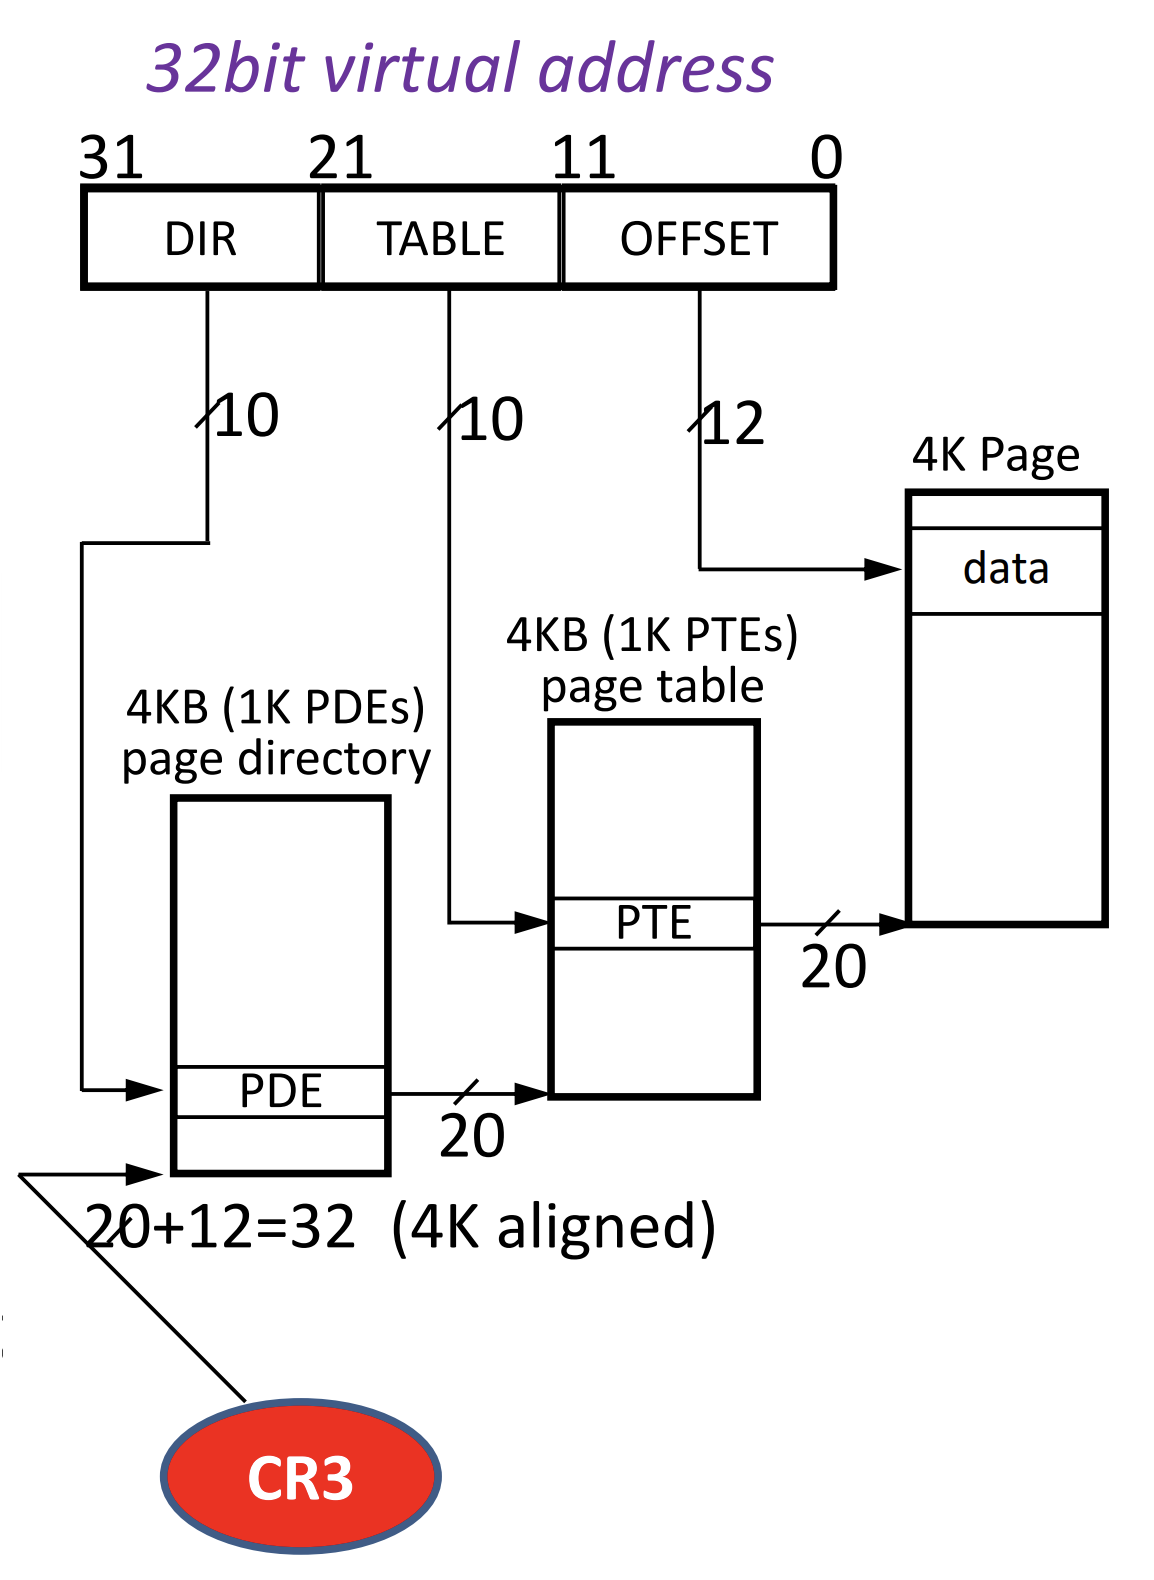
\includegraphics[width=\textwidth]{32bit-virtual.png}
        \caption{32-bit Page Tables}
        \label{fig:32bit-virtual}
    \end{subfigure}
\end{figure}


\paragraph{Global + User/Supervisor bits} The "user/supervisor" bit is used to indicate that only the OS (ring 0) can access the page, while user processes (ring 3) cannot. The "global" bit is used to indicate that the page is shared across all processes and should not be flushed from the TLB on context switches. This is used to implement shared kernel space across all memory spaces. 


\paragraph{HW/OS Cooperation} HW defines the data structures (hierarchy, PTE bits, etc.). While the OS determines most of the content of page directories \& page tables (setting the values \& mappings). The HW sets the bits of dirty and accessed, and does the \blue{table walk} automatically:
\begin{enumerate}
  \item If VA\(\Longrightarrow\)PA translation not found in TLB, "TLB miss"
  \item HW knows where to find the root page directory (CR3 register)
  \item HW walks the tables, hierarchially, until it reaches the data page
  \item It inserts the VA\(\Longrightarrow\)PA mapping into the TLB
\end{enumerate}
The HW populates the TLB, and the OS invalidates TLB entries when needed (e.g. on context switches, or when a page is evicted from memory). The OS is also responsible for Synchronizing between TLBs of different cores (TLB shootdown).


\subsection*{64-bit x86 address translations}
\paragraph{64-bit x86 address translations} 64-bit address means \(2^{64}\) physical addresses, which is \blue{16 Exabytes} of physical memory space. The virtual address is only 48-bits, which is \(2^{48}\) virtual addresses, which is \blue{256TB} of virtual memory space. The page size is still \(4KB\), but the PTE is now 8 bytes (64 bits) instead of 4 bytes (32 bits). The page table structure is similar to the 32-bit x86 architecture, but with additional levels of indirection.

\begin{figure}[H]
    \centering
    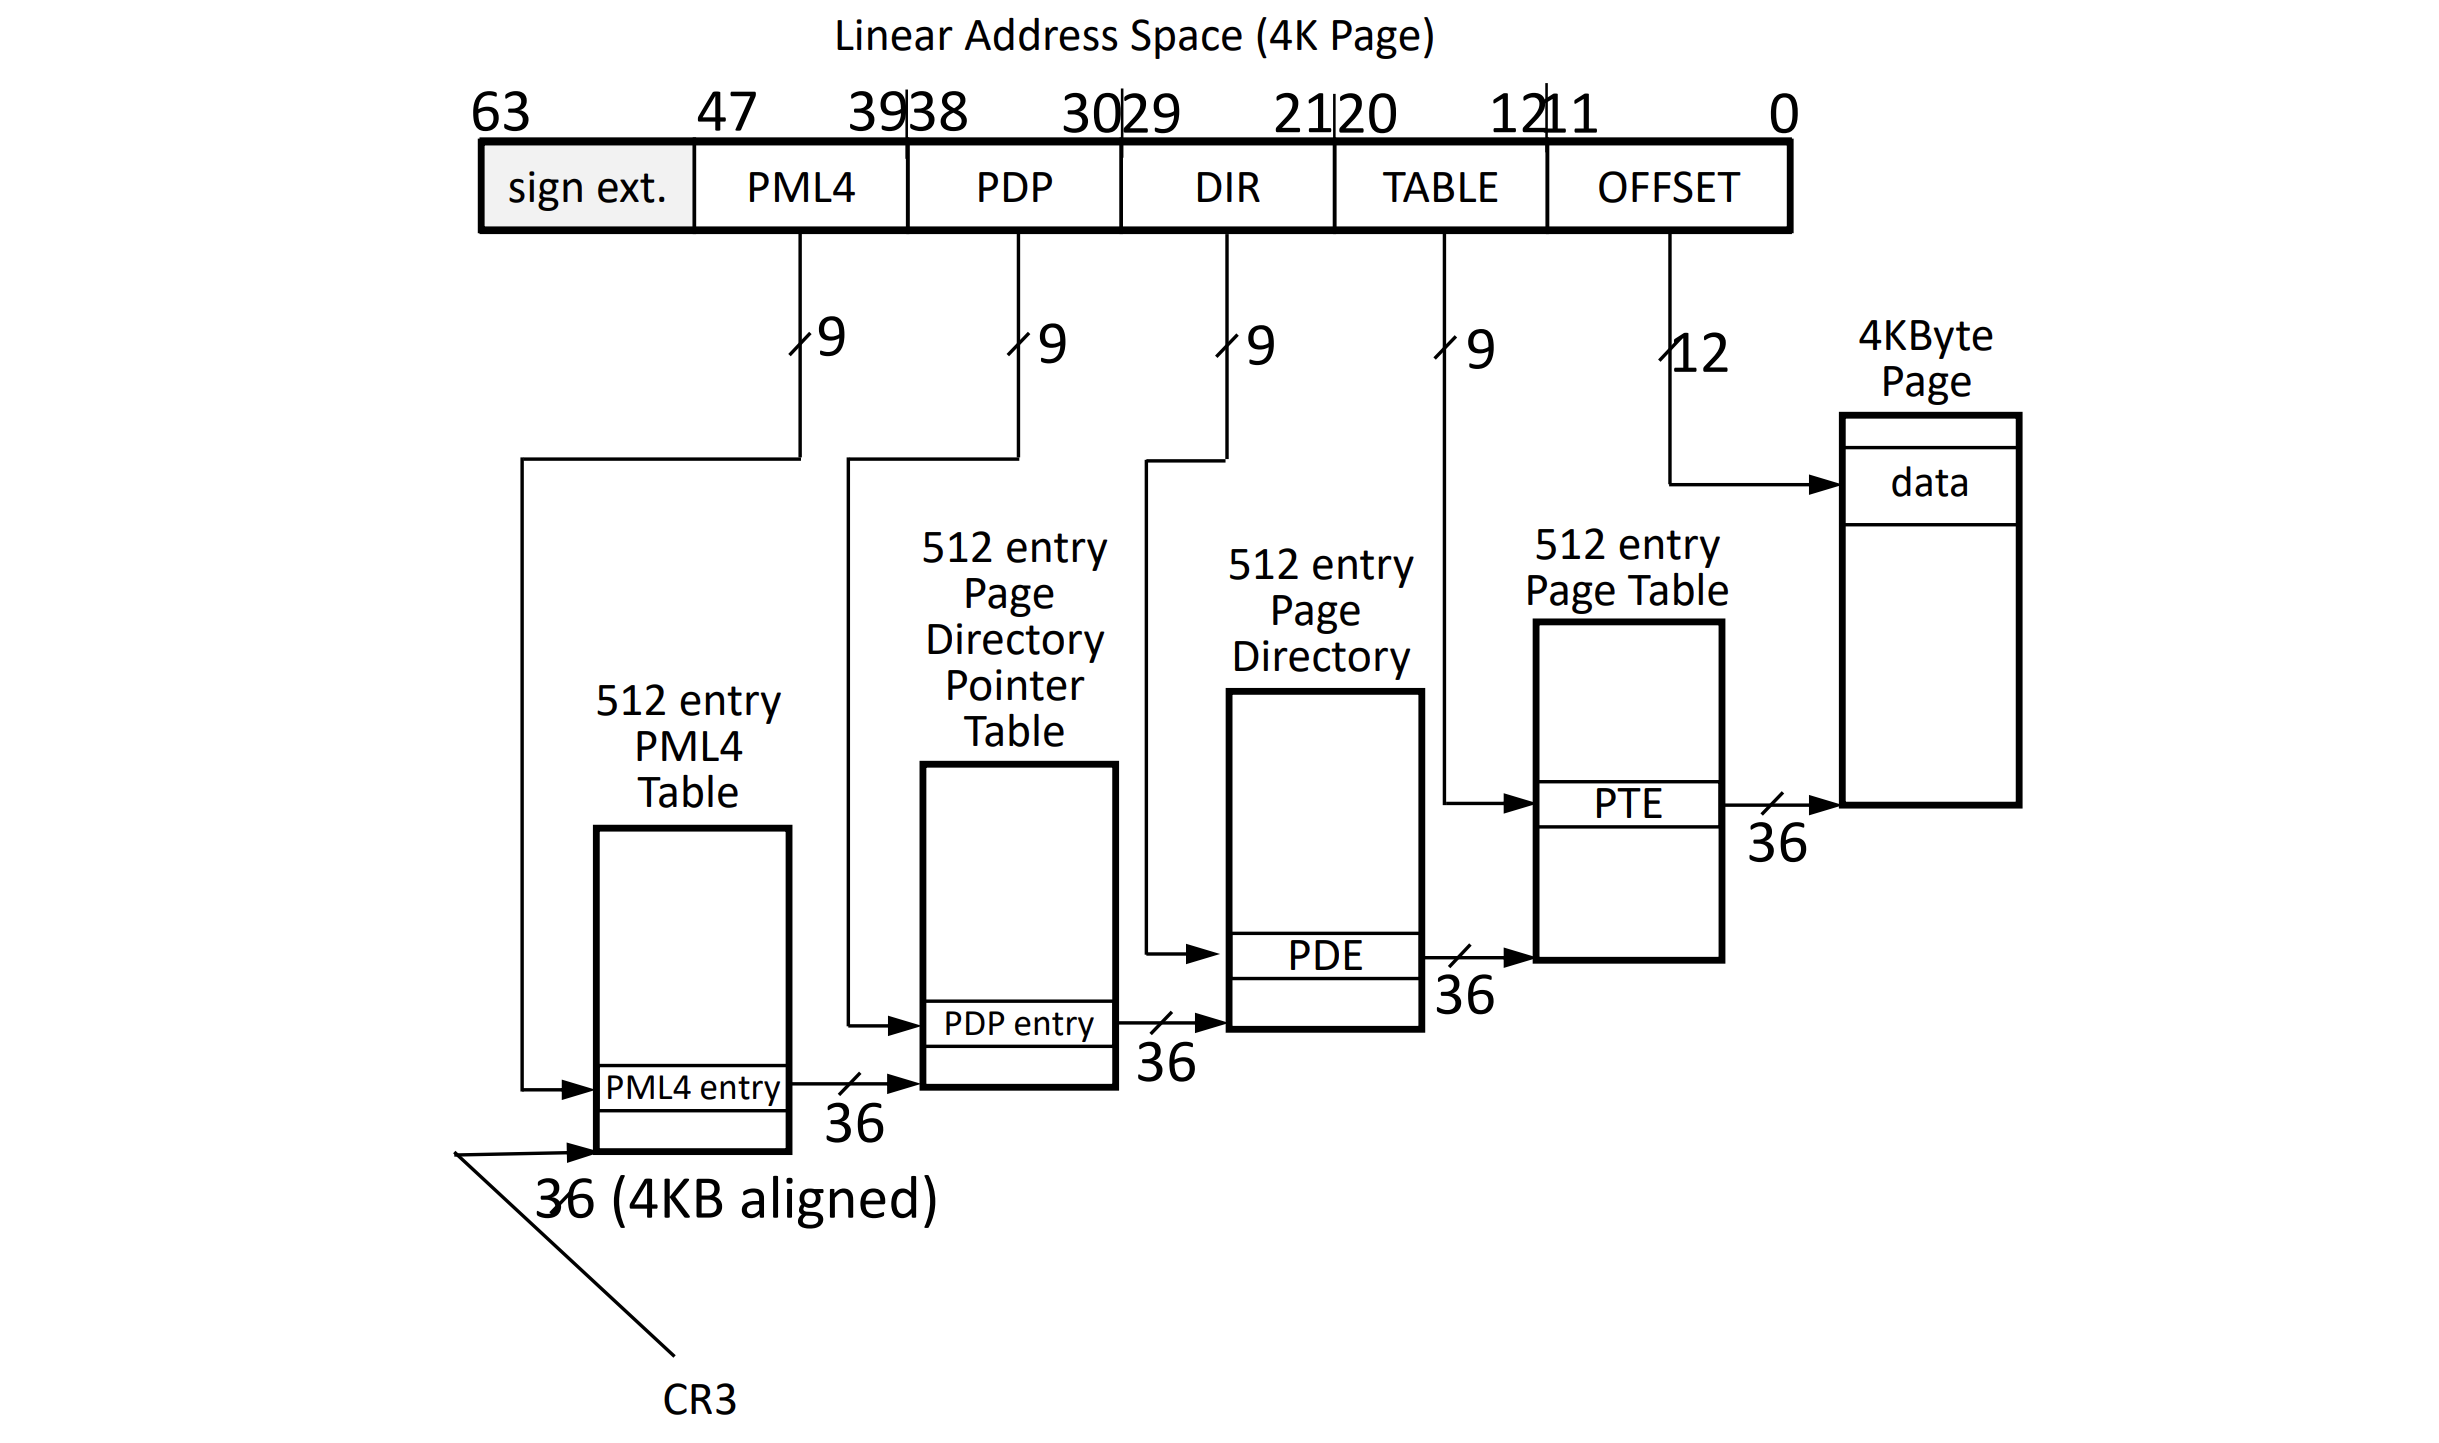
\includegraphics[width=0.8\textwidth]{64bit-tables.png}
    \caption{64-bit Page Tables}
\end{figure}



\paragraph{Increased TLB convergence} To make the TLB more useful we use two concepts:
\begin{itemize}
  \item TLB hierarchy: We use multiple TLB caches (like the L1, L2, ...) each bigger but slower than the last. Usually we use only two levels.
  
  \item \textbf{Superpages/Hugepages:} Different sizes are supported by different architectures;
  \begin{itemize}
    \item 32-bit x86: 4KB, 4MB pages
    \item 64-bit x86: 4KB, 2MB, 1GB pages
  \end{itemize}
  We merge the last \(N\) levels of page table bits in the VA into one offset of the superpage, allowing us to have fewer page table levels but larger pages.
\end{itemize}


\subsection*{64-BIT Power-PC (PPC) Virtual Memory}

A completely different architecture, but similar concepts, used in IBM PowerPC processors. 


\paragraph{3 Address Types} effective \(Longrightarrow\) virutal \(Longrightarrow\) real
\begin{itemize}
  \item \textbf{Effective:} Each process uses \blue{64-bit} effective addresses, which are not unique across processes. The equivalent of virtual addresses in x86.
  \item \textbf{Virtual:} A huge \blue{80-bit} address space, which is unique and shared by all processes. If two processes have the same effective address, they will can different virtual addresses, but if they have the same virtual address, they will have the same real address.
  \item \textbf{Real:} The actual physical address in memory, which is \blue{62-bit} addresses.
\end{itemize}

\paragraph{PPC Segments} Effective \& virtual spaces are partitioned into \textbf{segments}, which are \blue{256MB} in size. Each segment is contiguous in the per-process effective address space, and each segment is contiguous in the virtual address space. 


\paragraph{PPC SLB (Segment Lookaside Buffer)} The SLB is a cache used to speed up the translation of effective addresses to virtual addresses. \red{OS} manages the SLB, and HW searches the SLB for the effective address. Upon a miss, the OS is notified, and it will insert right segment table entry (STE) to SLB. Upon context switch, the OS invalidates the SLB entries. 

\paragraph{PPC TLB (Translation Lookaside Buffer)} The TLB is a cache used to speed up the translation of virtual addresses to real addresses. The TLB is managed by both OS \& HW. The virtual addresses are shared so no need to invalidate the TLB upon context switch.

\paragraph{PPC ERAT (Effective-to-Real Address Translation)} The ERAT is a cache used to speed up the translation of effective addresses to real addresses. Analogous to the TLB (in x86). 

\paragraph{PPC HTAB (Hash Table)} The HTAB is a hash table used to store the mappings between virtual addresses and physical addresses. Each PTE contains both PPN \& VPN, and the OS uses a hash function to map the VPN to a PPN. PTEs are divided into \textbf{PTEG} (Page Table Entry Groups), each containing 16 PTEs. Each PTE can either reside in a "primary" or a "secondary" PTEG. If a PTE is missing, a page-fault interrupt is raised, and the OS will place the PTE in either the primary or secondary PTEG.




\begin{figure}[H]
\centering
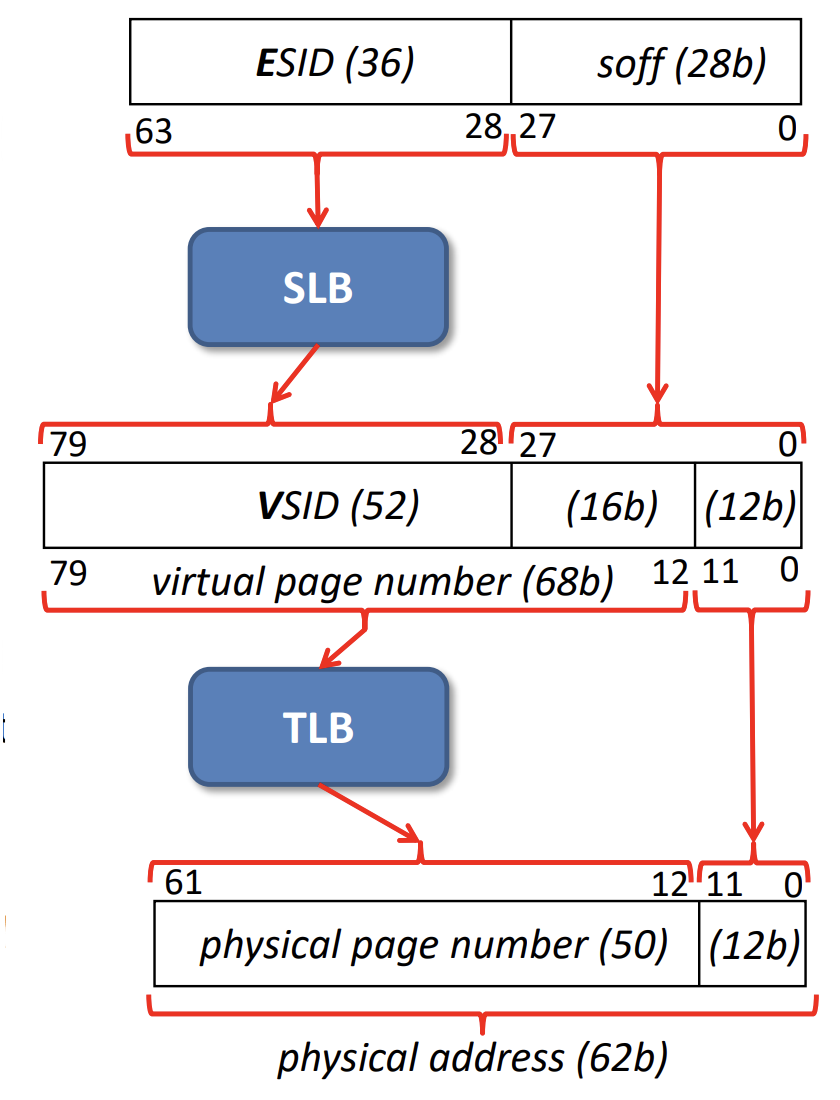
\includegraphics[width=0.4\textwidth]{PPC-Caches.png}
\caption{PPC Virtual Memory Architecture}
\label{fig:PPC-virtual-memory}
\end{figure}













\section*{Linux Implementation (OS)}


\paragraph{Memory Descriptor} The memory descriptor \blue{(\code{mm\_struct})} is a data structure used by the Linux kernel to manage a process's memory. It contains information about the process's virtual memory layout, including the location and size of each memory region. \ul{Threads share} the same memory descriptor, while processes have their own memory descriptor.  

\begin{figure}[H]
\centering
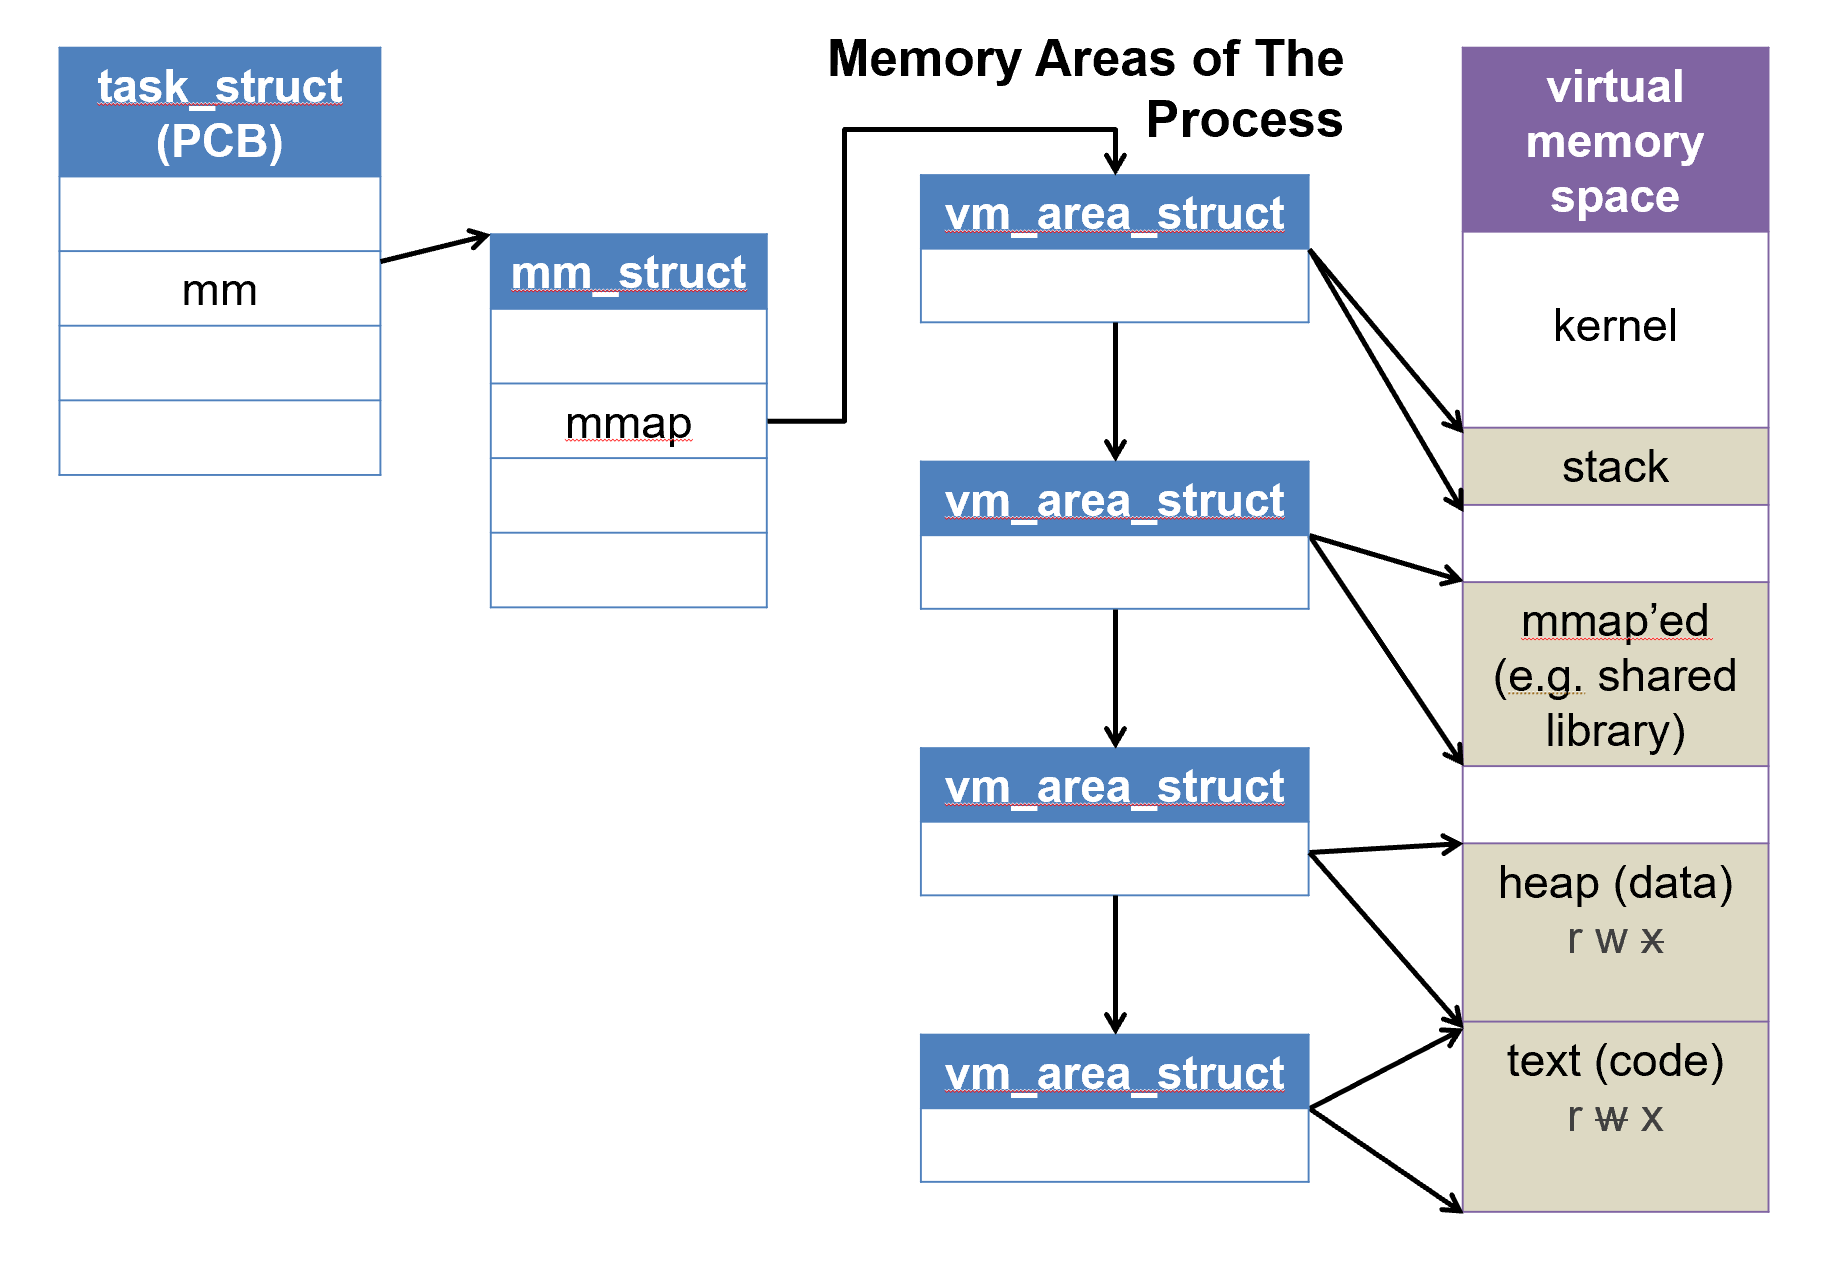
\includegraphics[width=0.6\textwidth]{memory_struct.png}
\caption{Memory Descriptor Structure in Linux}
\label{fig:memory-descriptor}
\end{figure}


\paragraph{Kernel Threads} are threads created by the operating system to execute specific tasks in the kernel space. E.g \code{kswapd} thread is responsible for managing memory by swapping pages in and out of physical memory. Kernel threads \red{do not have their own memory descriptor}, they point to \red{NULL}, so they keep the memory descriptor of the last process that was running (in CR3).

\blue{Every} kernel thread has his \blue{own kernel stack} in the kernel space, thus it does not need a memory descriptor of its own. They use the page tables of the last process, since \ul{kernel space exists (the same) in all user spaces}.


\paragraph{Kernel vs User Space} In x64-bit intel we use 48-bit virtual memory (256TB) and 52-bit physical memory (4PB). The kernel space is the upper half of the virtual address space, while the user space is the lower half. The kernel space is reserved for the operating system and its kernel threads, while the user space is reserved for user processes. The kernel space is not accessible by user processes, and vice versa. The kernel space is shared by all processes thus ensuring it can be accesses at any point from the kernel, using the page tables of the user process.







\paragraph{Memory Descriptor Fields} The memory descriptor contains several fields, including:
\begin{itemize}
  \item \textbf{\code{mm\_users}} - The number of \textit{*user*} processes that share this memory descriptor. 

  \item \textbf{\code{mm\_count}} - The number of \textit{*kernel*} threads + (all user process counter together as 1, if exist) that share this memory descriptor.

  \begin{itemize}
    \item If \code{mm\_users==0} then the OS frees all memory regions of the user (stack, heap, etc)

    \item If \code{mm\_count==0} then the OS frees the memory descriptor, and the page tables.
  \end{itemize}

  \item \textbf{\code{mmlist}} - Pointer (of type \code{list\_head}) to the global list of all memory descriptors.

  \item \textbf{\code{pgd}} - The root addresss of the page tables, the value loaded to CR3.

  \item \textbf{\code{mmap}} - Sorted linked list of the memory regions used (fig. \ref{fig:memory-descriptor}). 

  \item \textbf{\code{rss}} - The number of frames \textit{in use} by the process in the DRAM.

  \item \textbf{\code{total\_vm}} - The total number of virtual pages allocated by the process, including those that are not in DRAM (e.g. not allocated yet, or swapped out).
\end{itemize}



\paragraph{Memory Regions} The memory descriptor contains a linked list of memory regions, each represented by a \code{vm\_area\_struct} structure. Memory regions structs contain the following fields:
\begin{enumerate}
  \item \textbf{\code{vm\_start}} -  The starting virtual address of the memory region.
  
  \item \textbf{\code{vm\_end}} - The ending virtual address + 1 of the memory region.

  \item \textbf{\code{vm\_next}} - Pointer to the next memory region in the linked list.

  \item \textbf{\code{vm\_mm}} - Pointer back to the memory descriptor that this region belongs to.

  \item \textbf{\code{vm\_flags}} - Flags that describe the memory region, such as:
  \begin{itemize}
    \item VM\_READ, VM\_WRITE, VM\_EXEC - Access rights for the region (read, write, execute).

    \item VM\_MAYREAD, VM\_MAYWRITE, VM\_MAYEXEC - Upper values of the access rights, indicating whether the region can have these rights or not (can their access rights be set or not).

    \item VM\_SHARED - Indicates that the memory region is shared between processes 

    \item VM\_LOCKED - Prevents swapping out the memory region, ensuring it remains in physical memory.
  \end{itemize}

  \item \textbf{\code{vm\_page\_prot}} - The bit values to be set in all PTEs of this region.
\end{enumerate}





\begin{samepage}
\begin{center}
    
    % Define a custom column type for the content cells to ensure text wraps
    % and has consistent formatting.
    \newcolumntype{L}{>{\raggedright\arraybackslash}p{6.5cm}}
    
    % Set the row spacing to make the table less cramped
    \renewcommand{\arraystretch}{2.5}
    
    % Start alternating row colors from the first data row (the second row overall)
    \rowcolors{2}{gray!15}{white}
    
    \begin{tabular}{| l | L | L |}
        \hline
        % --- Header Row ---
        % This row is colored manually to override the \rowcolors command
        \rowcolor{blue!50}
        \multicolumn{1}{|c|}{\textcolor{white}{}} & 
        \multicolumn{1}{c|}{\textcolor{white}{\textbf{Anonymous}}} & 
        \multicolumn{1}{c|}{\textcolor{white}{\textbf{Named (File-Backed)}}} \\
        \hline

        % --- Row 1: Private ---
        \blue{\textbf{Private}} & 
        Not backed by any file + Exclusive to a single process.
        \newline\newline\textbf{Use Case:} A process's heap (\texttt{malloc}) and stack. On \texttt{fork()}, these pages are handled with Copy-on-Write (CoW).
        & 
        The page is initialized with data from a file, but modifications are private to the process and are not written back to the original file (Copy-on-Write).
        \newline\newline\textbf{Use Case:} Loading a file into memory using \texttt{mmap} with \texttt{MAP\_PRIVATE}.
        \\
        \hline

        % --- Row 2: Shared ---
        \blue{\textbf{Shared}} &
        Shared between multiple processes but not associated with any file on the filesystem. All processes see the same physical page of memory.
        \newline\newline\textbf{Use Case:} Inter-Process Communication (IPC) where processes need a fast shared memory segment without needing a temporary file, E.g \textit{pipes}.
        &
        The page is initialized with data from a file, and it is shared among multiple processes. Any modifications are visible to all processes and are written back to the underlying file.
        \newline\newline\textbf{Use Case:} Created with \texttt{mmap} with \texttt{MAP\_SHARED}. The disk updates every few seconds, in batches, to avoid performance issues, or using \texttt{fsync(fd)} to force immediate write.
        \\
        \hline
    \end{tabular}
    \textbf{Classification of Memory Pages}
\end{center}
\end{samepage}


Note: Heap + Stack pages are always \textit{anonymous} pages, and they are always \textit{private} to the process. Code (text) region is always \textit{named} (file-backed) and \textit{shared} between processes.


Note 2: \code{execv()} replaces the current process's memory with a new program, effectively replacing all \code{vm\_area\_struct}s in the memory descriptor with new ones.


\paragraph{More on CoW (Copy on Write)} 
When a process forks, the OS creates a new memory descriptor for the child process, and new page tables. For each memory region, the OS copies the \code{vm\_area\_struct} of the parent to the child process, then copies the PTE from the parent to the child. For each frame used by the parent process (\ul{that is private + writable}), the OS adds the counter of threads using the frame and unsets the write access for this page from everyone.

Upon write access we hit a page fault, if the \code{vm\_area\_struct} allows writing (\code{VM\_WRITE} is on), then the OS copies the frame to a new one to allow writing (if this was the last thread then it doesn't copy as there is no need, it just sets the write access on).

Note: CoW doesn't always improve performance, as if we copy all of the memory page by page, it would have been more efficient to copy it all at once.





% =====================================================
% =============== Lecture Interrupts ==================
% =====================================================



\newpage
\Topic{Interrupts}

\paragraph{Interrupts \& Exceptions} Our intterupts are Intel's interrupts and exceptions, such that: exceptions = internal (synchronous) implicit interrupts, and interrupts = all the rest. There are two sources for intterupts:
\begin{enumerate}
  \item \textbf{External / Asynchronous} - Triggered by devices external to the core's compute circuitry. Assynchronous because they can occur at any time.

  \item \textbf{Internal / Synchrounous} - Triggered by the core's compute ciruitry (CPU intructions). Sometimes called "Software interrupts" as they are triggered by the CPU executing an instruction.
\end{enumerate}

\paragraph{Internal Interrupts} Internal interrupts can be further divided into:
\begin{itemize}
  \item \textbf{Explicit} - Triggered by the CPU executing an instruction that deliberately causes an interrupt, such as \code{int} instruction, or \code{syscall} instruction, or \code{Ptrace}-ing.

  \item \textbf{Implicit} - Triggered by the CPU executing an instruction that causes an error or \blue{exception}, such as division by zero, invalid memory access, or illegal instruction. i.e. the CPU can't complete the instruction so it transfers control to the OS. Two types of exceptions:
  \begin{itemize}
    \item \textbf{Error condition} tells the OS that the app did something illegal.
    \item \textbf{Temporary problem} such as a page fault, which can be resolved by the OS.
  \end{itemize}
\end{itemize}


\paragraph{Interrupt Handling} Each interrupt is associated with a Number (called \blue{interrupt vector}), which is used to identify the \blue{interrupt handler}. Handlers are pointed to by and \blue{\code{array[256]} of pointers-to-functions}. The interrupt handler saves the state of the current running procesess and then executes the handler.

\paragraph{Context Type} If the interrupt is \red{asynchronous} then the kernel is said to be in \blue{interrupt context}, meaning it doesn't server the process that has just been stopped. If the interrupt is \red{synchronous} then the kernel is in \blue{process context} as it needs to provide some service to the process that invoked it.


\vspace*{0.5em}

\red{NOTE:} interrupt handlers are not schedulable entities, they run immediately (without invoking the scheduler), unless the interrupt is masked. We can mask using a bitmap, incase of maksing an interrupt the HW will remember at most \red{2} instances of each interrupt that was blocked by the mask (the rest get lost, if they exist).


\paragraph{Top \& Bottom Halves} Interrupt handling is often divided into two parts: the \textbf{top half} and the \textbf{bottom half}. The top half is the part of the interrupt handler that runs in response to the interrupt and does the minimal amount of work necessary to handle the interrupt. The bottom half is the part of the interrupt handler that can be deferred and run later, allowing the top half to return quickly and minimize the impact on the system's responsiveness.


\paragraph{Resuming an interrupted process} We split to multiple cases:
\begin{itemize}
  \item \textbf{Asynchronous (external) interrupts:} Resume in the next process instruction, right after the last instruction that was exectued. Note that asynchronous interrupts are caught and handled between instructions.

  \item \textbf{Synchronous (=internal) + explicit:} Likewise, resume in the next instruction.

  \item \textbf{Synchronous (=internal) + implicit:} Resume in the \red{same} instruction that caused the HW failure, called \blue{restartable instruction}. For temporal problems the OS will fix the problem, but for error conditions it doesn't make sense so a signal will also be sent to the process.
\end{itemize}


\paragraph{Interrupt handling in multicores} Internal (synchronous) interrupts are always handled by the core that executed the instruction that caused the interrupt. External (asynchronous) interrupts can be handled by any core, so we can do any kind of partition between the cores (static/dynamic/...).


\paragraph{Polling} Polling is a technique used to check the status of a device or resource at regular intervals. In the context of interrupts, polling can be used as an alternative to interrupts for handling events. Instead of relying on the hardware to generate interrupts, the CPU actively checks the status of devices and resources to determine if they require attention. This can be useful in situations where interrupts are cause an \blue{interrupt storm} (too many interrupts in a short time), leading to performance degradation. 


\paragraph{Interrupt Coalescing} The hardware tries to not create an "interrupt storm" by coalescing multiple events into a single interrupt. And the Software also temporarily switches to polling mode when the flow of incoming intterupts exceeds a certain thershold.

\paragraph{DMA \& interrupts} DMA = Direct memory access, which is when an I/O device can directly read/write to memory without involving the CPU. Conceptually devices fire an interrupt when a DMA operation is finished, not only when reciving (reading) data, but also when sending (writing) data. This allows to notify OS when the send buffer has become free.


\red{Note:} All interrupts are handled in \blue{kernel mode}, CPL=0, including the timer interrupt.




\begin{samepage}
  \begin{center}
  \rowcolors{2}{gray!15}{white}
  \begin{tabular}{|>{\raggedright\arraybackslash}p{6.5cm}|
  >{\raggedright\arraybackslash}p{6.5cm}|}
  \hline
  \rowcolor{blue!30}
  \textbf{System Calls / Exceptions} & \textbf{Hardware Interrupts} \\
  \hline
  If the processor is running user code, a system call or exception transitions control to the kernel for handling.
  &
  The kernel immediately handles any incoming hardware interrupt, even if it is already in the middle of handling an exception, system call, or another interrupt.
  \\
  \hline
  System calls can be blocking and cause the process to yield the processor (e.g., \texttt{read()}, \texttt{wait()}).
  &
  A hardware interrupt handling routine never yields the processor.
  \\
  \hline
  Handling for a system call or exception can be preempted by an incoming hardware interrupt.
  &
  An interrupt handler will not make system calls or cause exceptions (with the exception of a page fault). After handling the interrupt, the kernel may switch to a different process than the one that was previously running.
  \\
  \hline
  \end{tabular}
  \end{center}
 \end{samepage}




\paragraph{Kernel Control Paths} A kernel control path is block of instructions that the kernel uses to handle: (1) Syscalls, (2) Hardware Interrupts, (3) Exceptions. Different control paths can interleave with each other as follows:



\begin{samepage}
  \begin{center}
    \rowcolors{2}{gray!15}{white}
    \begin{tabular}{|>{\raggedright\arraybackslash}p{6.5cm}|
      >{\raggedright\arraybackslash}p{6.5cm}|}
      \hline
      \rowcolor{blue!30}
      \textbf{System Calls / Exceptions} & \textbf{Hardware Interrupts} \\
      \hline
      A handler for a system call or exception will \red{not} cause a new exception (with the notable exception of a page fault).
      &
      An interrupt handler will \red{not} make a system call or cause an exception (other than a page fault). After handling is complete, the kernel may schedule a different process to run.
      \\
      \hline
      \textbf{Single Processor:} the handler can be preempted by a hardware interrupt, and it can interleave with all other control paths.
      &
      \textbf{Single Processor:} the handler can only interleave a different hardware interrupt handler.
      \\
      \hline
      \textbf{Multi-Processor:} the handlers can interleave with each other, from all control paths.
      &
      \textbf{Multi-Processor:} the handlers can interleave with each other, from all control paths.
      \\
      \hline
    \end{tabular}
  \end{center}
\end{samepage}


\paragraph{Disabling Interrupts} Disabling interrupts is a technique used to prevent the kernel from being interrupted by hardware interrupts while executing critical sections of code. This is typically done to ensure that the code can execute atomically without being preempted. However, disabling interrupts can lead to performance issues and should be used sparingly.

To disable an interrupt we set the flag \blue{\code{IF}} in the \code{RFLAGS} register to 0, and to enable it we set the flag to 1. In critical code, we turn off the \code{IF}, but at the end we set it back to the \ul{previous value}. 




\begin{figure}[H]
\centering

% Define common styles for both TikZ pictures to ensure consistency
\tikzset{
    % Set distances between nodes: vertical and horizontal
    node distance=1cm and -0.5cm,
    % Style for decision boxes (blue rectangles)
    decision/.style={
        rectangle, 
        draw, 
        thick,
        fill=blue!20, 
        text width=3.5cm, 
        text centered, 
        minimum height=2cm,
        font=\sffamily
    },
    % Style for action boxes (green rounded rectangles)
    answer/.style={
        rectangle, 
        rounded corners, 
        draw, 
        thick,
        fill=green!20, 
        text width=3.5cm, 
        text centered, 
        minimum height=2cm,
        font=\sffamily
    },
    % Style for arrows
    arrow/.style={
        draw,
        thick,
        -Stealth % Arrow tip style
    }
}

%---------------------------------
% First Diagram (Original Image)
%---------------------------------
\begin{minipage}{0.48\textwidth}
    \centering
    \textbf{One Core CPU}
    \vspace{0.5cm} % Add some space below the header
    
    % The 'scale' option makes the entire figure smaller
    \begin{tikzpicture}[scale=0.75, transform shape]
        % Layer 1
        \node[decision] (q1) {Is the data structure accessible to hardware interrupts?};

        % Layer 2
        \node[answer, below left=of q1] (a1) {Disable local interrupts}; 
        \node[decision, below right=of q1] (q2) {Is the data structure accessible to exceptions or system calls?};

        % Layer 3
        \node[answer, below=of q2] (a2) {Semaphore lock};

        % Arrows
        \path[arrow] (q1) -- node[above, sloped] {Yes} (a1);
        \path[arrow] (q1) -- node[above, sloped] {No} (q2);
        \path[arrow] (q2) -- node[left] {Yes} (a2);
    \end{tikzpicture}
\end{minipage}%
\hfill % Adds flexible space between the two diagrams
%---------------------------------
% Second Diagram (New Image)
%---------------------------------
\begin{minipage}{0.48\textwidth}
    \centering
    \textbf{Multi-Core CPU}
    \vspace{0.5cm} % Add some space below the header
    
    % The 'scale' option makes the entire figure smaller
    \begin{tikzpicture}[scale=0.75, transform shape]
        % Layer 1
        \node[decision] (q1) {Is the data structure accessible to hardware interrupts?};

        % Layer 2
        \node[answer, below left=of q1] (a1) {Disable local interrupts + \red{spinlock}};
        \node[decision, below right=of q1] (q2) {Is the data structure accessible to exceptions or system calls?};

        % Layer 3
        \node[answer, below=of q2] (a2) {Semaphore lock};

        % Arrows
        \path[arrow] (q1) -- node[above, sloped] {Yes} (a1);
        \path[arrow] (q1) -- node[above, sloped] {No} (q2);
        \path[arrow] (q2) -- node[left] {Yes} (a2);
    \end{tikzpicture}
\end{minipage}

\end{figure}

























% =====================================================
% ==================== Page Cache =====================
% =====================================================



\newpage
\Topic{Page Cache}

\paragraph{Page Cache} The page cache is a memory area used by the operating system to cache disk pages in RAM. It is used to speed up disk I/O operations by keeping frequently accessed pages in memory, reducing the need to read from or write to the disk. The page cache is managed by the operating system and is transparent to user processes.


Every I/O operation on the disk is done via the page cache; If the page is already on the page cache (in DRAM) (either from the process, or a different process) then it will use said page, else it will obtain the page from the disk and place it in the page cache.


\paragraph{Write-Back} write ops to the disk are delayed and done in batches. This allows for minimising the number of disk access ops, but at the cost of validicy since data on the disk is not correct at all times.


\paragraph{Read-Ahead} If the kernel recognizes a sequential pattern of accesses to the file, it will preemptively read the next few pages into the page cache. This allows for less page-faults, but might waste memory on wrong predections.



\paragraph{Frame Table} The frame table is a data structure used by the operating system to manage physical memory pages. It keeps track of which physical pages are in use, which are free, and their associated metadata. Each entry in the frame table corresponds to a physical page frame in memory and contains information as follows:
\begin{itemize}
  \item \textbf{\code{refcount}} - How many memory spaces point to this frame.

  \item \textbf{\code{mapping}} - Pointer to the inode this frame belongs to, NULL in case of anonymous frame.

  \item \textbf{\code{index}} - The offset in the file this frame corresponds to, empty in case of anonymous frame.

  \item \textbf{\code{flags}} - Flags that describe the frame, such as: PG\_dirty, PG\_active, PG\_referenced.

  \item \textbf{\code{next\_hash}, \code{prev\_hash}} - Pointers to the next/previous frames in the page hash table (explained next).
\end{itemize}



\paragraph{Page Hash Table} The page hash table is a data structure used by the operating system to manage the mapping (\code{mapping} + \code{index}) to frames in the DRAM. All conflicting hashes are connected using chain-hashing, with the pointers \code{next\_hash},\code{prev\_hash} from the frame table.



\begin{figure}[h!]
\centering
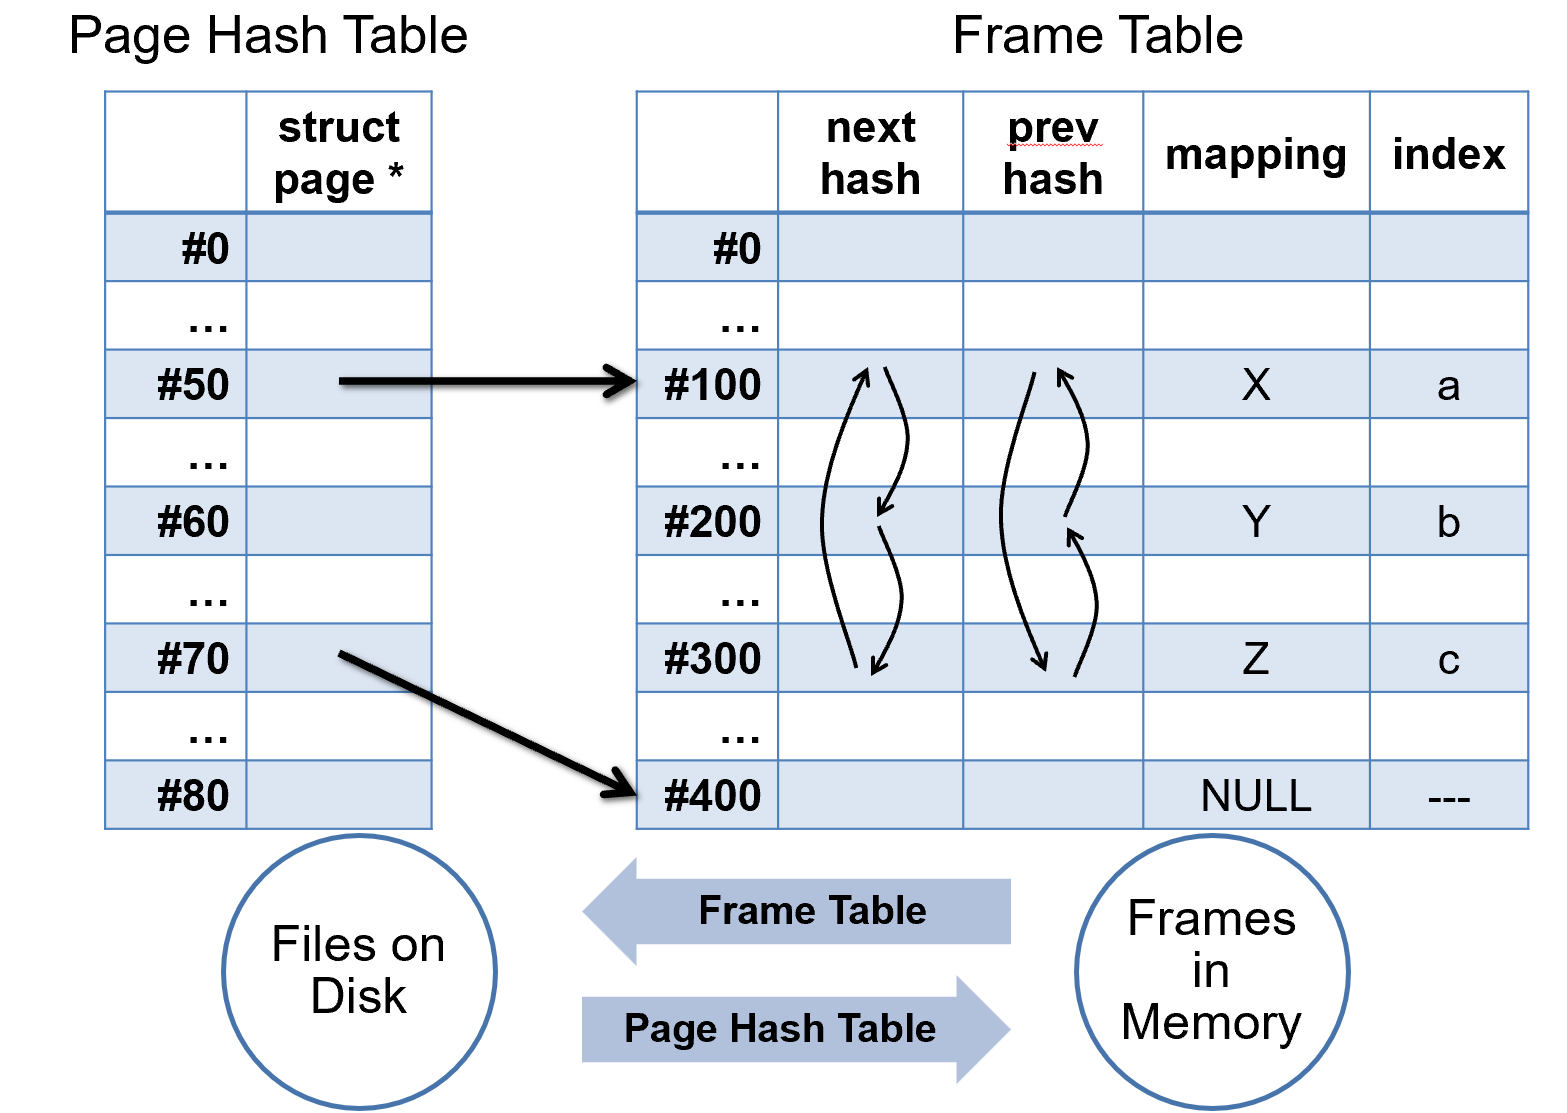
\includegraphics[width=0.7\textwidth]{Frame-Table.png}
\caption{Frame Table + Page Hash Table; Note: that both structures are implementted in software, not in hardware}
\label{fig:frame-table}
\end{figure}






\paragraph{mmap vs read/write} \texttt{mmap} and traditional \texttt{read/write} operations are two different methods for performing file I/O.

\begin{itemize}
    \item \textbf{read/write System Calls}:
    \begin{itemize}
        \item The system call brings data from the disk into the page cache.
        \item It then copies the relevant data from the page cache to the user's buffer.
    \end{itemize}

    \item \textbf{mmap System Call (File Mapping)}:
    \begin{itemize}
        \item The system call creates a new memory region but does not read data from the disk at that time.
        \item It uses lazy/deferred memory management.
        \item An attempt to access the mapped memory region will cause a page fault. This fault prompts the system to read the data from the disk into the page cache and then updates the page table to point directly to the frames within that page cache.
    \end{itemize}
\end{itemize}


\paragraph{PFRA (Page Frame Reclaim Algorithm)} The PFRA is a mechanism used by the operating system to manage the page cache and reclaim memory when needed:
\begin{itemize}
  \item Page cache pages (named pages): If the page is dirty (modified), it is written back to the disk before being reclaimed. If it is clean, it is simply removed from the page cache.
  \item Anonymous pages: These pages are not backed by any file and therefore must be backed to the swap area before removing them, whether dirty or clean.
\end{itemize}


\red{Note:} PFRA only reclaims (frees) \ul{user} pages, and \ul{never kernel} pages.

Note 2: Multiple swap areas can exist, improving performance by parallelizing the swap operations. 

Note 3: As mentioned earlier, the swap area is the only area in the disk that is partitioned to slots of 4KB isntead of blocks of 512B.


\paragraph{When to Swap?} PFRA runs according to the amount of the free pages in the memory based on:
\begin{itemize}
  \item if \(free\_pages > pages\_high\): Stop running PFRA. Reason: To not free too many pages and hurt performance.

  \item if \(free\_pages < pages\_low\): Start running PFRA in background asynchronously (\blue{\texttt{kswapd} thread}). Reason: To lower the time of new allocation requests (making available space in advance)

  \item if \(free\_pages < pages\_min\): Start running PFRA synchronously, in foreground, blocking processes that try to allocate memory until enough pages are reclaimed. Reason: PFRA requires memory to run, if the number of free pages is below a certain threshold, the kernel might crash.
\end{itemize}




\begin{figure}[H]
  \centering
  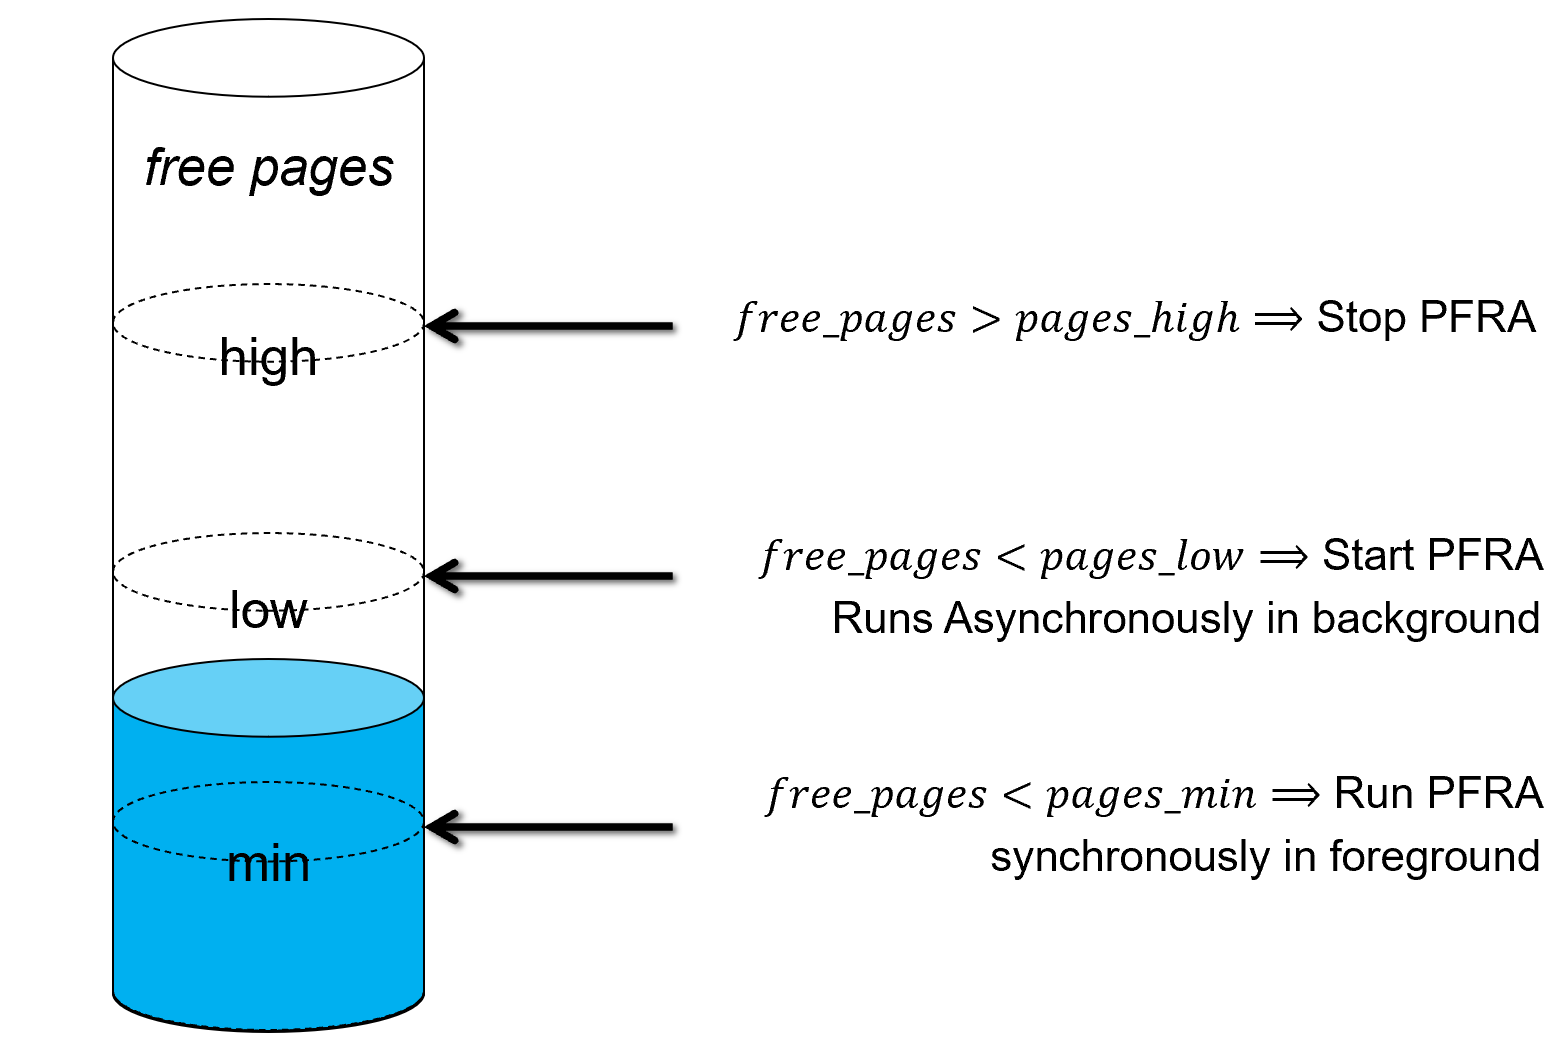
\includegraphics[width=0.7\textwidth]{PFRA.png}
  \caption{PFRA swap limits}
  \label{fig:PFRA}
\end{figure}



\paragraph{PFRA Rules} The PFRA uses the following rules to decide which pages to reclaim:
\begin{enumerate}
  \item Prefer freeing \textit{page cache pages} that are not in use by any process (i.e., pages with a \code{refcount} of 0) or/and clean pages (not dirty).

  \item Dynamically follow the level of activity of the pages, and prefer freeing "cold" pages (i.e., pages that have not been accessed recently).

  \item Freeing shared frames must be done atomically at once from all processes that share the frame.
\end{enumerate}

Note: Anonymous pages can't be "not pointed to by processes" because they will be freed as soon as they are not used anymore.




\paragraph{Page Replacement Algorithms} using an intelligent page replacement policy helps with virtual memory performance:
\begin{itemize}
  \item \textbf{Belady - Optimal} - (theoretical) Replace the page that will not be used for the longest period of time in the future. 

  \item \textbf{LRU (least recently used)} - (impractical) Replace the page that has not been used for the longest period of time in the past. 

  \item \textbf{Clock} - (practical LRU) A circular list of pages in memory, where each page has a reference bit. When a page is accessed, its reference bit is set to 1. When a page needs to be replaced, the algorithm checks the pages in a circular manner, clearing the reference bit of each page until it finds a page with a reference bit of 0, which is then replaced.

  \item \textbf{NRU (not recently used)} - (practical more sophisticated LRU) Keep to bits for each page, dirty \& referenced, and periodically turn off referenced (as in clock). Replace victim page with the lowest class from the following: (class 0) not referenced, not dirty, (class 1) not referenced, dirty, (class 2) referenced, not dirty, (class 4) referenced, dirty. 

  \item \textbf{PFRA (page frame reclaim algorithm)} - (used) As mentioned, each frame keeps flags for \code{PG\_referenced} and \code{PG\_accessed} (the latter is set by the hardware on each access). Both bits together define a level of activity (as seen in fig. \ref{fig:PFRA}), where lower activity pages are more likely to be reclaimed. At each access, the kernel increments the activity level, and we periodically decrement the activity (to prevent long history). We keep all frames in an \code{active} list and an \code{inactive} list, and we move frames between the lists based on their activity level.

\end{itemize}


\begin{figure}[H]
  \centering
  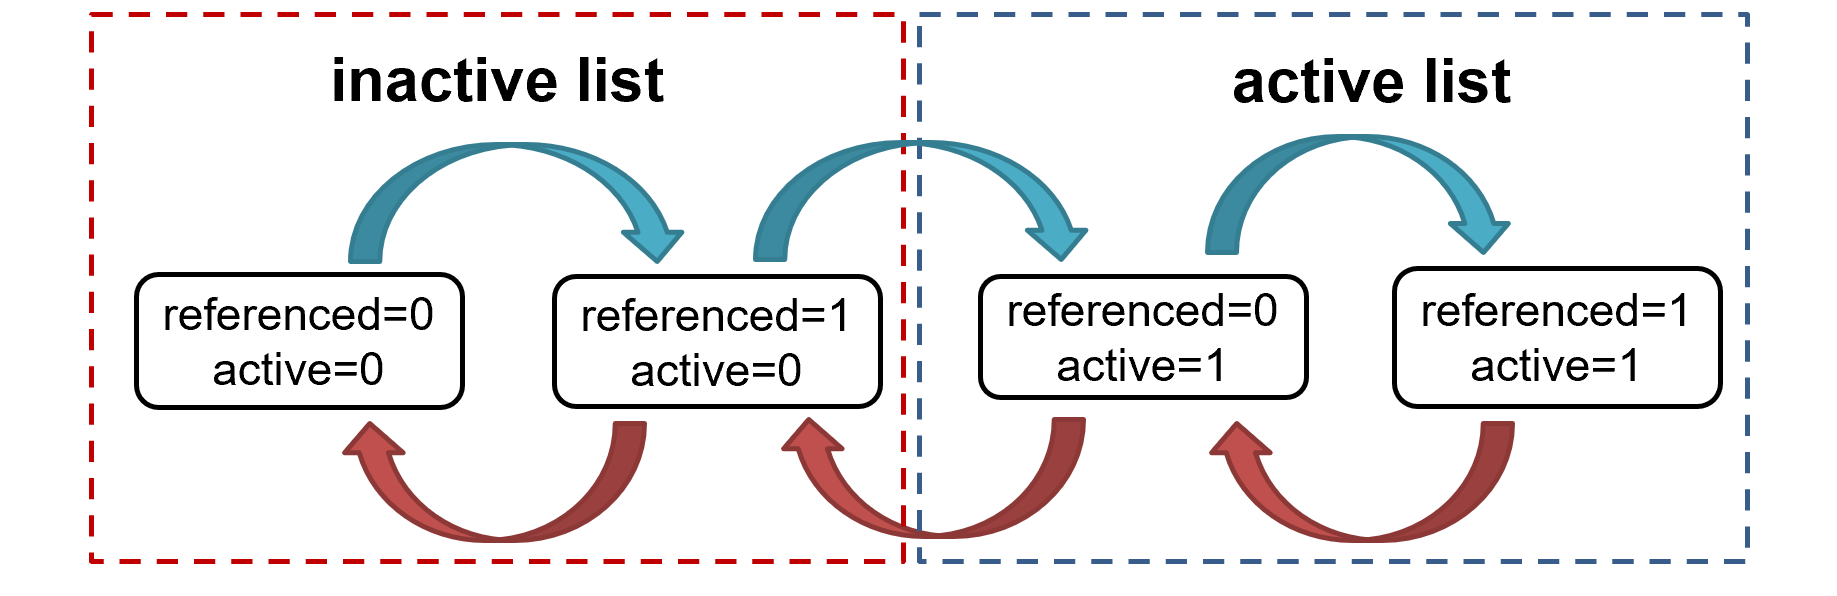
\includegraphics[width=0.9\textwidth]{PFRA-Lists.png}
  \caption{PFRA swap limits}
  \label{fig:PFRA-lists}
\end{figure}





% =====================================================
% ================= Lecture Storage ===================
% =====================================================



\newpage
\Topic{Storage}


\section*{Files \& Directories}

\paragraph{File} A file is a logical unit of information which is an ADT (abstract data type), with a name, content, metadata, and can be manipulated via operations (read, rename,...)

\paragraph{File Metadata} Metadata is information about the file and its content, such as: (1) file name, (2) file size, (3)  owner, (4) permissions, (5) timestamps (creation, modification, access), (6) physical location, (7) file type.

\paragraph{File Descriptors} A file descriptor (FD) is a nonnegative integer that uniquely identifies an open file within a process. An FD is an index into a per-process file descriptor table (FDT), which maps the FD to a file object in the kernel. \blue{Threads share} the FDT of their process. Some POSIX syscalls operate on FDs and others operate on file names (chmod, unlink, ...).

\paragraph{File Operations} The following are the most common file operations:
\begin{itemize}
    \item \textbf{Creation} (syscalls: \texttt{creat}, \texttt{open}; C: \texttt{fopen})
    \begin{itemize}
        \item Associate with a name; allocate physical space (at least for metadata)
    \end{itemize}

    \item \textbf{Open} (\texttt{open}; C: \texttt{fopen}, \texttt{fdopen})
    \begin{itemize}
        \item Load required metadata to allow process to access file
    \end{itemize}

    \item \textbf{Deletion} (\texttt{unlink}, \texttt{rmdir}; C: \texttt{remove})
    \begin{itemize}
        \item Remove name/file association \& (possibly) release physical content
    \end{itemize}

    \item \textbf{Close} (\texttt{close}; C: \texttt{fclose})
    \begin{itemize}
        \item Mark end of access; release associated process resources
    \end{itemize}

    \item \textbf{Rename} (\texttt{rename}; -)
    \begin{itemize}
        \item Change associated name
    \end{itemize}

    \item \textbf{Stat} (\texttt{stat}, \texttt{lstat}, \texttt{fstat}; -)
    \begin{itemize}
        \item Get the file's metadata (timestamps, owner, etc.)
    \end{itemize}

    \item \textbf{Chmod} (\texttt{chmod}, \texttt{fchmod}; -)
    \begin{itemize}
        \item Change readable, writable, executable properties
    \end{itemize}
    
    \item \textbf{Chown} (\texttt{chown}, \texttt{fchown}; -)
    \begin{itemize}
        \item Change ownership (user, group)
    \end{itemize}

    \item \textbf{Seek} (\texttt{lseek}; C: \texttt{fseek}, \texttt{rewind})
    \begin{itemize}
        \item Each file is typically associated with a "current offset"
        \item Pointing to where the next read or write would occur
        \item \texttt{lseek} allows users to change that offset
    \end{itemize}

    \item \textbf{Read} (\texttt{read}, \texttt{pread}, \texttt{readv}; C: \texttt{fscanf}, \texttt{fread}, \texttt{fgets})
    \begin{itemize}
        \item Reads from "current offset"; \texttt{pread} gets offset from caller
        \item Need to provide buffer \& size
        \item "v" = vector of buffer+size; this version is called "scatter-gather" (why?)
    \end{itemize}

    \item \textbf{Write} (\texttt{write}, \texttt{pwrite}, \texttt{writev}; C: \texttt{fprintf}, \texttt{fwrite}, \texttt{fputs})
    \begin{itemize}
        \item Change content of file; \texttt{pwrite} gets the offset explicitly; v=vector
        \item Likewise, need to provide buffer \& size
        \item If the current offset (or the given offset in the case of \texttt{pwrite}) points to end of file, then file grows
    \end{itemize}

    \item \textbf{Sync} (\texttt{sync<fs>}, \texttt{fsync<fd>}; $\neq$ C: \texttt{fflush})
    \begin{itemize}
        \item Recall that
        \begin{itemize}
            \item All disk I/O goes through OS "page cache", which caches the disk
            \item OS sync-s dirty pages to disk periodically (every few seconds)
        \end{itemize}
        \item Use this operation if we want the sync now
        \item `sync` is for all the filesystem, and `fsync` is just for a given FD
        \item Sync $\neq$ fflush; the latter flushes user-space (\texttt{fprintf}, \texttt{cout}) buffers to the kernel
    \end{itemize}

    \item \textbf{Lock} (\texttt{flock}, \texttt{fcntl}; C: \texttt{flockfile})
    \begin{itemize}
        \item "Advisory" lock (= processes can ignore it, if they wish)
        \item There exists mandatory locking support (in Linux and other OSes)
        \begin{itemize}
            \item E.g., every open implicitly locks; and can't open more than once
        \item But that's not POSIX
        \end{itemize}
    \end{itemize}
\end{itemize}

\paragraph{File Types} In UNIX (POSIX) we classify files into:
\begin{itemize}
  \item \textbf{Regular files} - Contain user data, such as text files, binary files, etc. They are the most common type of file.
  \item \textbf{Directories} - Special files that contain a list of files and
  \item \textbf{Symbolic links (soft links)} - Special files that point to another file or directory, allowing for easy access to files in different locations.
  \item \textbf{FIFOs (named pipes)} - Special files that allow for inter-process communication (IPC) by providing a way for processes to communicate with each other through a named pipe.
  \item \textbf{Sockets} - Special files that allow for communication between processes over a network. They are used for network communication and can be either stream-oriented (TCP) or datagram-oriented (UDP).
  \item \textbf{Device files} - Special files that represent hardware devices, such as disks, printers, and terminals. They allow processes to interact with hardware devices as if they were regular files. Can be either character devices (e.g., terminals) or block devices (e.g., disks).
\end{itemize}


\paragraph{Magic Numbers} Magic numbers are a semi-standard Unix way to tell the type of a file by looking at the first few bytes of the file. Each file type has a unique magic number that identifies it. For example, a PDF file starts with the ASCII string: \code{\%PDF}. Not all files have magic numbers, but many do, since nowadays it is a more complex scheme. 


\paragraph{File Protection (Ownership \& Mode)} For each file, POSIX divides users into 3 classes: "User" (the owner of the file), "group", "all" (all other users). Each class has 3 permissions: "read", "write", "execute". The file mode is a 9-bit number, where each bit represents a permission for a class. The first 3 bits are for the user, the next 3 bits are for the group, and the last 3 bits are for all users. \blue{Note:} Users can belong to several groups, but not files.

Other operating systems (NOT POSIX) use \blue{Access Control Lists (ACLs)}, where it allows a finer more detailed control of what each user/group can do (delete, rename,...).


\paragraph{Directories} A filesystem has a hierarchial (tree) structre of directories, where each directory can contain files and subdirectories. Each directory is a special file that contains a list of files and subdirectories, along with their metadata. 

\paragraph{Absolute \& Relative File Paths} \blue{File name = File path = path}. Every process has its own "working directory" (WD). A path is \blue{absolute} if it starts with \blue{"/"} (the root directory)\gray{, e.g. "/users/admin/jon"}. A path is \blue{relative} (to the WD) otherwise\gray{, e.g. if WD="/home" then "admin/jon" is the relative to "/home/admin/jon".}


\paragraph{Directory Operations} Each directory contains 2 special subdirectories, \blue{"."}=Current directory, \blue{".."}=Parent directory. To create a directory we use \code{mkdir}, and to remove an empty one \code{rmdir}.



\paragraph{Hard Links} \red{File \(\neq\) file name}. They are \red{not} the same thing, in fact, the name is \red{not} even part of the file's metadata! A file can have multiple names, and therefore appearing in multiple unrelated places. Every file has a "reference count" to keep track of how many hard links it has, once it reaches zero, \textit{if no process is using it through FDs}, then and only then we can remove the file's content. 

Hard links to directories are usually disallowed, since it causes infinite circular looping and nesting. However, remember that each directory contains "." \& ".." hence each directory has a minimum of 2 hard links, and a maximum depending on the number of subdirectories it contains.

\red{Note:} Hard links can only exist on the same filesystem, as they use the same \code{file\_object} \gray{or as seen later, same \code{inode}}.

\paragraph{Symbolic Links} A symbolic link (or soft link) is a special file that points to another file or directory. It is a way to create a shortcut to a file or directory, allowing you to access it from a different location. Symbolic links are not hard links, and they can point to files or directories that do not exist. \textbf{Soft links contain target file path, and not a pointer to a file object like hard links}. They are no counted in the target file's ref count, they can refer to files, directories, and even files outside the filesystem. (since they only save a path)


When applying a syscall to a symlink, the syscall is applied to the target file. Except, (1) unlink, which removes the soft link. (2) symlink-specific syscall, such as symlink \gray{(create a symlink)} and readlink \gray{(read the content of the symlink, i.e. the path of the target file)}.



\paragraph{inode} An inode (index node) is a data structure used to represent a file in a filesystem. Each file has its own (single) inode, which can be thought of as the "file". File names (hard links) point to inodes, and the inode contains all metadata of the file.

Note: file objects (which represent open files) are not the same as inodes, as they contain additional information such as the current offset, number of file descriptors pointing to it, etc. However, file objects point to the inodes, as they are the ones holding to the actual data.

\paragraph{inode \code{*stat} syscall} POSIX gurantees that at leas the following fields will be found in the stat structure and have meaningful values:

\begin{tabular}{r l l}
1. & \texttt{st\_dev} & ID of device containing file \\
2. & \texttt{st\_ino} & inode number, unique for st\_dev \\
3. & \texttt{st\_mode} & specifies file type \& permissions (S\_ISREG(m), ... \\
4. & \texttt{st\_nlink} & number of hard links to the file \\
5. & \texttt{st\_size} & file size in bytes \\
6. & \texttt{st\_uid} & user ID of owner \\
7. & \texttt{st\_gid} & group ID of owner \\
8. & \texttt{st\_ctime} & last time \blue{metadata (=inode) or data \textbf{changed}} \\
9. & \texttt{st\_mtime} & last time \blue{data \textbf{modified}}  \\
10. & \texttt{st\_atime} & last time \blue{metadata (=inode) or data \textbf{accessed}} \\
11. & \texttt{st\_blksize} & block size of this file object (preferred size for I/O ops) \\
12. & \texttt{st\_blocks} & number of sectors allocated for this file object \\
\end{tabular}

\textbf{\code{lstat}} is like \code{stat} but it applies to the symbolic links when used on one, i.e. it returns the metadata of the symlink, not the target file. The only guaranteed metadata fields to be found are: \code{st\_mode} \gray{(which will specify it is a symlink)} and \code{st\_size} \gray{(which will be the length of the symlink's target path)}.

\red{It is not} specified in POSIX whether a symlink gets an inode or not (could be either
 depending on implementaion).


\paragraph{Dirents (Directory Entries)} A directory file is compromised of directory entries (dirents), which point to the inodes of the files and subdirectories it contains. Each dirent contains the following fields: (1) inode number, (2) file type, (3) file name, (4) offset to the next dirent, (5) length of the dirent. In \textbf{FAT} \gray{(more on that later)} dirents are the actual files as there are no inodes, preventing multiple hard links.


\paragraph{Path Resolution} Resolving a path means finding the inode of the file or directory that the path points to. The algorithm that syscalls use to resolve paths is called \textbf{\blue{"namei"}}. Each path is compromised of "atoms", where an atom is a single file or directory name in the path. The algorithm works as follows:
\begin{lstlisting}[language=C, caption={Path Resolution Algorithm (namei)}, label={lst:namei}]
int my_open(char *fname) {
  if (fname is absolute){
    // Start from the root directory
    chdir("/");
    make fname relative;
  }
  foreach atom in fname do // e.g. atoms of "x/y" are "x" and "y"
    if (is symlink) SYS (fd = my_open(atom symlink target))
    else            SYS (fd = open(atom)) // this checks permissions too

    if (!terminal){
      // If not the last atom, change the current directory to the opened one
      chdir(fd directory);
      close(fd);
    }
    else
      // If terminal, return the file descriptor of the last opened file
      break;
  return fd;
}
\end{lstlisting}

For each non-symlink atom in the path, a user must be able to \ul{search} all directories leading to the file. This means that the user must have the appropriate permissions to access each directory in the path. \blue{x} bit = \textbf{search} allows the user to search for files in the directory. \blue{r} bit = allows the user to list the contents of the directory (with \code{ls} for example). \blue{w} bit = allows the user to create or delete files in the directory.


\paragraph{FDT \& GFDT} Each process has a \textbf{File Descriptor Table (FDT)}, which is an array of file descriptors that the process has opened. The FDT is indexed by file descriptor numbers, and each entry in the FDT points to a \textbf{File Object} in the kernel, which contains information about the open file, such as the current offset, the inode, and the file operations that can be performed on it. 

All opened files for every process in the system are saved in one global table, GFDT.

By default, every process has the following three standard FDs: (\code{fd=0}) STDIN, the standard input channel, (\code{fd=1}) STDOUT, the standard output channel, (\code{fd=2}) STDERR, the standard error channel.

\paragraph{file object} A file object is a kernel data structure that contains all the information about an open file, including its current offset, the inode it refers to, and the file operations that can be performed on it, the number of file descriptors pointing to it, the mode it was opened with, etc. 

\section*{File Systems}

Note: The CPU can't directly access/process data on the disk, it must reside on the DRAM.

\paragraph{HDD Latency} HDD latency is \textbf{seek time} + \textbf{rotational latency}. Seek time is the time it takes for the read/write head to move to the correct track on the disk. Rotational latency is the time it takes for the disk to rotate to the correct sector. 


\paragraph{Sectors \& Blocks} A disk is divided into \textbf{sectors}, which are the smallest addressable units on the disk. Each sector is typically \blue{512 bytes}\gray{ or 4096 bytes in size}. Sectors are grouped into \textbf{blocks}, which are the equivalent of pages in memory, thus each block is \blue{4KB} in size, and \blue{8 sectors}.

Note: Only the \ul{swap area} is divided into frames (like the memory) instead of sectors.

Note 2: The disk gurantees that operations on sectors are atomic, meaning that a read or write operation on a sector will either complete successfully or fail without leaving the sector in an inconsistent state.


\paragraph{Partitions \& Mounts} A disk can be divided into \textbf{partitions} using \code{fdisk}, which are contiguous disjoint part of the disk that can host a filesystem. Disks are typically names "/dev/sda","/dev/sdb", while partitions are named "/dev/sda1", "/dev/sda2", etc. 

To create an empty filesystem on a partition we use \blue{\code{mkfs}}, which then after it need to be \blue{\code{mount}}ed to make it accessible. Mounitng is done using \blue{\code{mount -t <filesystem> <partition> <path>}} which will then make the filesystem reachable from \code{<path>}. If any files existed at \code{<path>} before mounting, they will become unavailable until we unmount the filesystem.




\paragraph{\blue{VSFS} (Very Simple File System)} Blocks are divided into 5 categories:
\begin{itemize}
  \item \textbf{Superblock (S)} - Contains metadata about the filesystem, such as the magic number of the filesystem, the inode of the root directory "/", amount of inodes and data blocks, start of inode table, etc. It is used when mounting the filesystem.

  \item \textbf{Inode Table (I)} - Contains the inodes of all files in the filesystem.

  \item \textbf{Data Blocks (D)} - Contains the actual data of the files in the filesystem.

  \item \textbf{bitmap of allocated inodes (i)} - A bitmap that indicates which inodes are allocated and which are free. Each bit corresponds to an inode.

  \item \textbf{bitmap of allocated data blocks (d)} - A bitmap that indicates which data blocks are allocated and which are free. Each bit corresponds to a data block.
\end{itemize}

\begin{figure}[H]
    \centering
    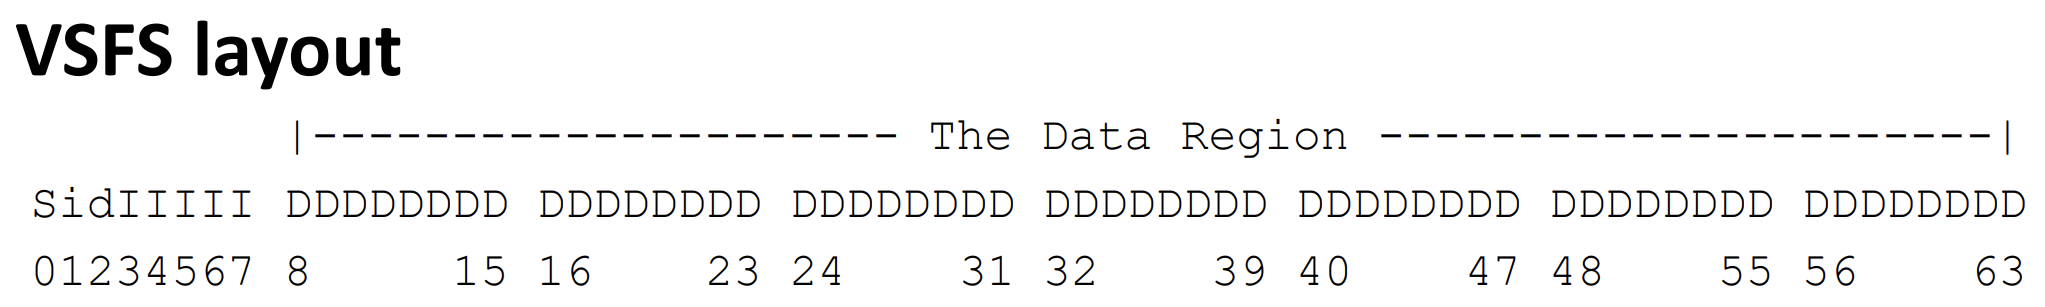
\includegraphics[width=0.8\textwidth]{VSFS_layout.png}
    \caption{VSFS File System Layout}
    \label{fig:vsfs}
\end{figure}

\paragraph{VSFS - Finding an inode} to find the address of an inode, we can simply do
\begin{equation*}
  \text{inodeAddr} = \text{inodeStartAddr} + \text{inodeSize} \times \text{inodeIndex}
\end{equation*}
and to find the block:
\begin{equation*}
  \text{blockAddr} = \text{inodeAddr}/\text{blockSize}
\end{equation*}

\paragraph{Pointers to data} in VSFS could be:
\begin{itemize}
  \item \textbf{Direct:} An array of pointers pointing directly to all data blocks (limited amount \(\Longrightarrow\) limits file size)

  \item \textbf{Indirect:} Multi-level array, like in virutal memory page tables.

  \item \textbf{Linked List:} Linked list of pointers from one data block to the next
\end{itemize}




\begin{center}
  \begin{minipage}[t]{0.6\textwidth}
    \vspace{0pt} % force top alignment
    \textbf{Multi-Level Index:} Each inode will have an array of \blue{15} pointers such that: (0-11) The first twelve are \blue{direct} pointers to data blocks, (12) a \blue{single-indirect} pointer that points to a block completely comprised of pointers to data blocks, (13) a \blue{double-indirect} pointer that points to a block that contains pointers to single-indirect blocks, and (14) a \blue{triple-indirect} pointer that points to a block that contains pointers to double-indirect blocks. \red{Note:} each indirect access requires an additional disk access, so it is slower than direct access. 
  \end{minipage}%
  \hspace{1em}
  \begin{minipage}[t]{0.35\textwidth}
    \vspace{0pt} % force top alignment
    \centering
    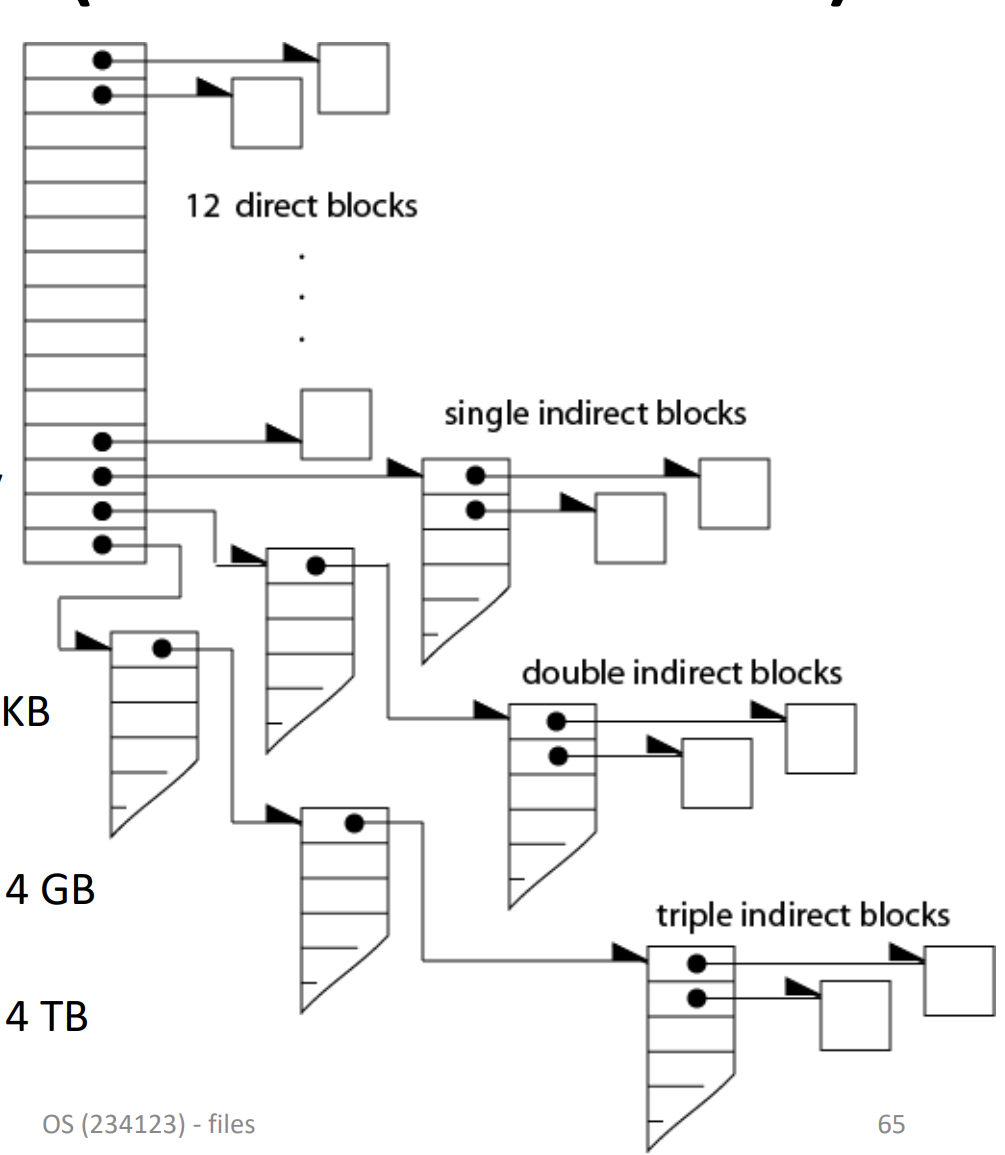
\includegraphics[width=0.8\textwidth]{multi-level-index.png}
  \end{minipage}
\end{center}




\paragraph{Extents} An extent is a contiguous block of data blocks that are allocated together. Instead of having a separate pointer for each data block, an extent is a single pointer that points to the first block of the extent and contains the length of the extent. This allows for more efficient allocation and reduces fragmentation. Extents are used in modern filesystems such as ext4. 

\begin{itemize}
  \item ext2 = the "extended file system", does not support extents, instead uses the multi-level index.
  \item ext3 = ext2 + journaling. journaling = keeping track of uncommitted changes.
  \item ext4 = ext3 + extents. (so "ext" name unrelated to "extent")
\end{itemize}


\paragraph{FAT (File Allocation Table)} Keeping track of a linked list using the data blocks is inefficient. So to solve that, FAT keeps a file allocation table that for each data block, it registers that pointer to the next data block from the same file. The starting block for the file is pointed to by the dirent, which holds all of the metadata too, so no inodes are needed! (but no multipicity of hard links is allowed)

The \green{advantage} for FAT is that it will be copied to (cached in) the memory, which allows fast lookup in the table. The \red{disadvantage} is that it can become huge.

In the FAT, 0=Free block, (-1)=Broken block (can't be used), (FF)=End of chain, (Other numbers)=Next block in the chain.



\section*{RAID}

\paragraph{RAID (Redundant Array of Independent Disks)} RAID is a technology that allows us to combine multiple physical disks into a single logical disk. It is based on \blue{striping}, which is the process of dividing data into blocks and distributing them across multiple disks. And \blue{redundancy}, which is the process of storing multiple copies of data to protect against disk failures. 


\begin{itemize}
  \item \textbf{RAID 0} - Striping without redundancy.\\
  \begin{itemize}
    \item   Files are stripped in \textbf{block} resolution.
    \item   Pros: Increased performance, as multiple disks can be accessed in parallel.
    \item   Cons: No redundancy, if one disk fails, all data is lost. and increased chance of failure.
  \end{itemize}

  \item \textbf{RAID 1} - Mirroring.\\
  \begin{itemize}
    \item Files are striped across half the disks, and each block is mirrored on the other half. 
    \item Pros: Increased reliability, as data is stored on multiple disks. Read performance is as good as RAID 0.
    \item Cons: Write performance is slower than RAID 0, as data must be written to multiple disks.
  \end{itemize}

  \item \textbf{RAID 4} - Dedicated parity disk.\\
  \begin{itemize}
    \item Data blocks are striped across multiple disks, and a dedicated parity disk is used to store parity information. \gray{RAID 2 is bit resolution, RAID 3 is byte resolution.}
    \item Pros: Improved read performance, as data can be read from multiple disks in parallel. Fault tolerance, as data can be reconstructed from parity information.
    \item Cons: \textbf{"small write problem"}, as writing to a single block requires reading the old data + the parity block, computing the new parity, and writing both the data and the parity block. However, if we write to the entire stripe (whole block on each disk) then we don't have to read the parity to update it, hence "small write problem".
  \end{itemize}

  \item \textbf{RAID 5} - Distributed parity.\\
  \begin{itemize}
    \item Data is striped across multiple disks, and parity block is distributed each time on a different disk.
    \item Pros: Like RAID 4 + No hotspot disk.
  \end{itemize}

  \item \textbf{RAID 6} - Double distributed parity.\\
  \begin{itemize}
    \item Data is striped across multiple disks, and two independent parity blocks are distributed across the disks.
    \item Pros: Fault tolerance for up to two disk failures, as data can be reconstructed from the remaining disks. 
    \item Cons: wastes \(2/N\) instead of \(1/N\) of the disk space for parity (compared to RAID 5).
  \end{itemize}

  \item \textbf{RAID n+k} - n data blocks and k parity blocks (in each stripe).
\end{itemize}

\paragraph{Erasure (n+k) vs. Replication (r)} Erasure is the "k parity" blocks, which allows us to reconstruct the data from the remaining blocks. Replication is duplicating the data \(r\) times. Erasure is less wasteful but slower, while replication is faster but more wasteful.







% ==================================================== 
% ==================================================== 
% ==================================================== 
% ----------------- Summary Section ------------------
% ==================================================== 
% ==================================================== 
% ==================================================== 
\newpage
\part{Overall Summary}




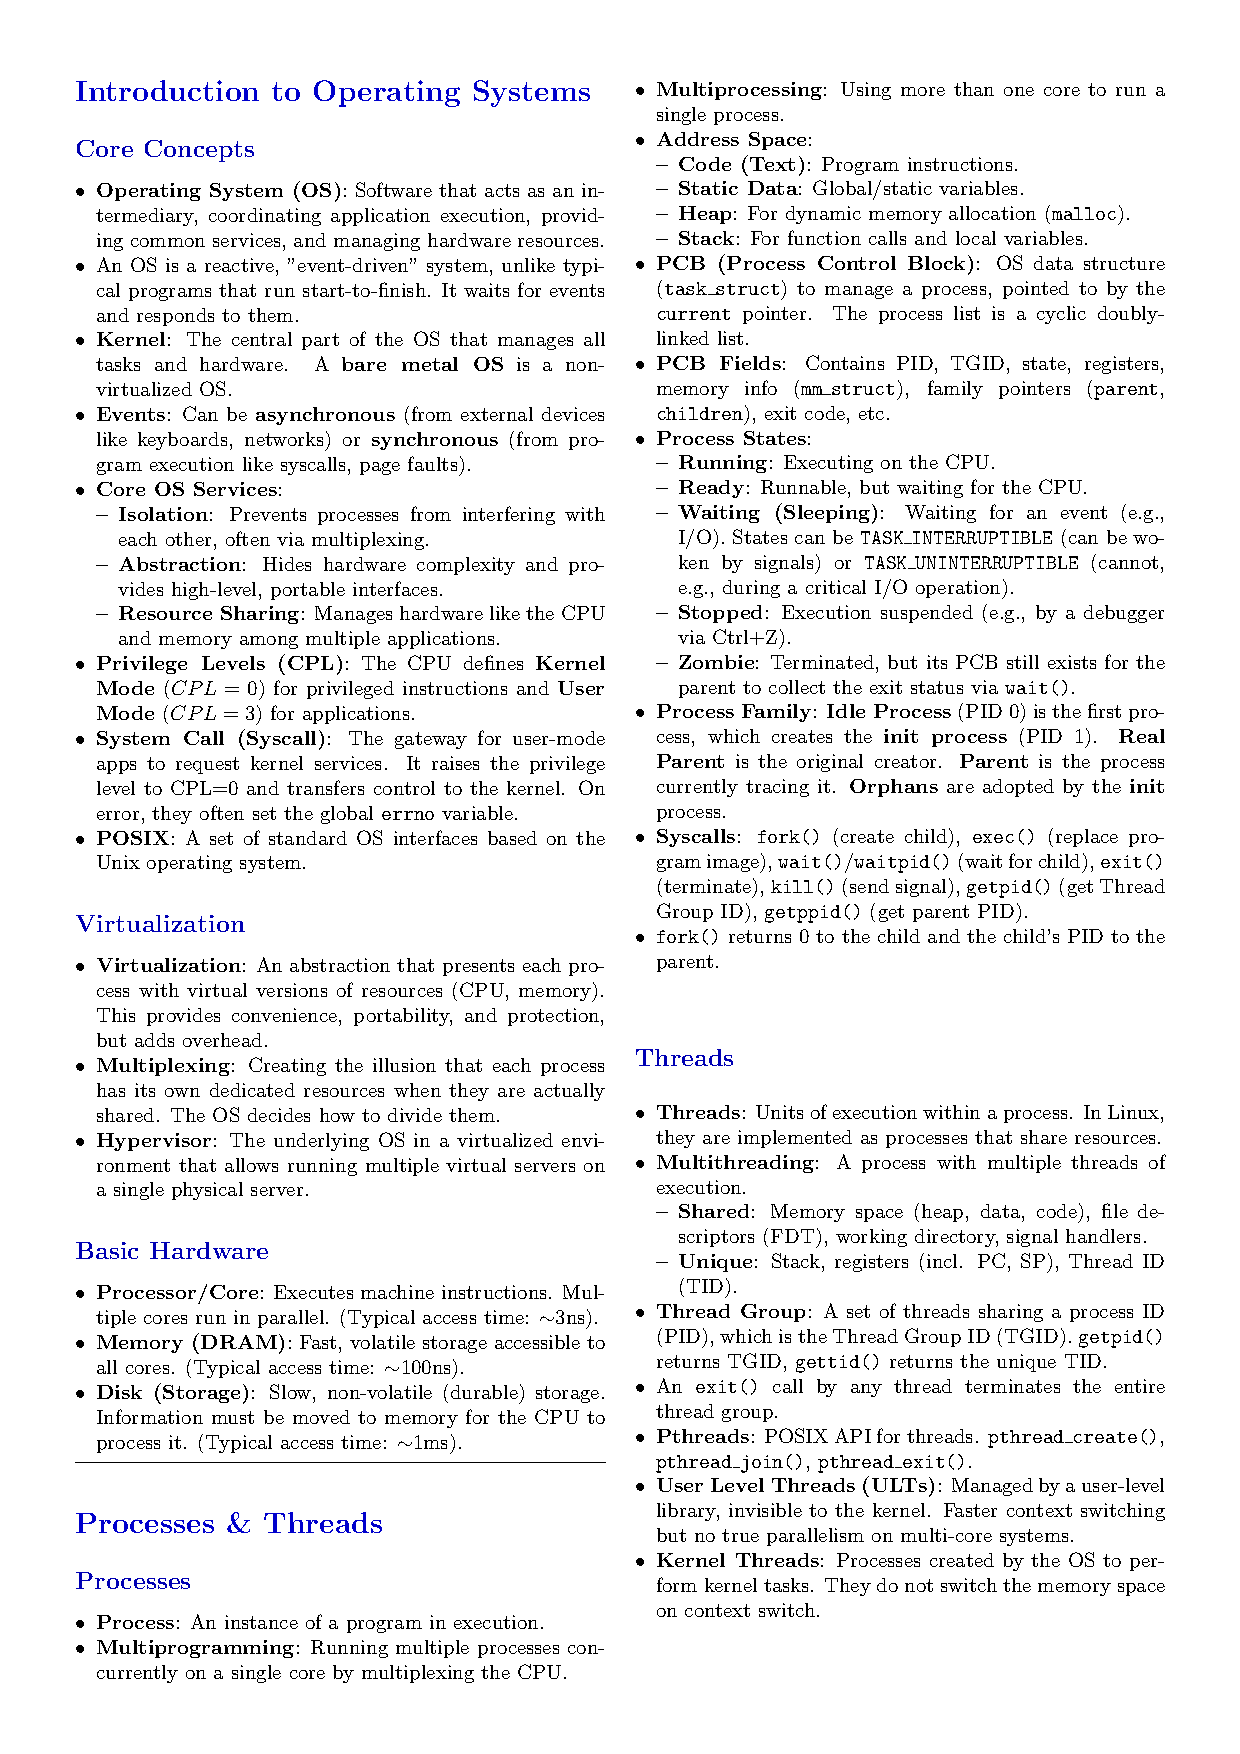
\includepdf[pages=-]{../Compressed Summary/compressed summary.pdf}








% ==================================================== 
% ==================================================== 
% ==================================================== 
% --------------- Highlights Section ----------------=
% ==================================================== 
% ==================================================== 
% ==================================================== 
\newpage
\part{Highlights and Notes}





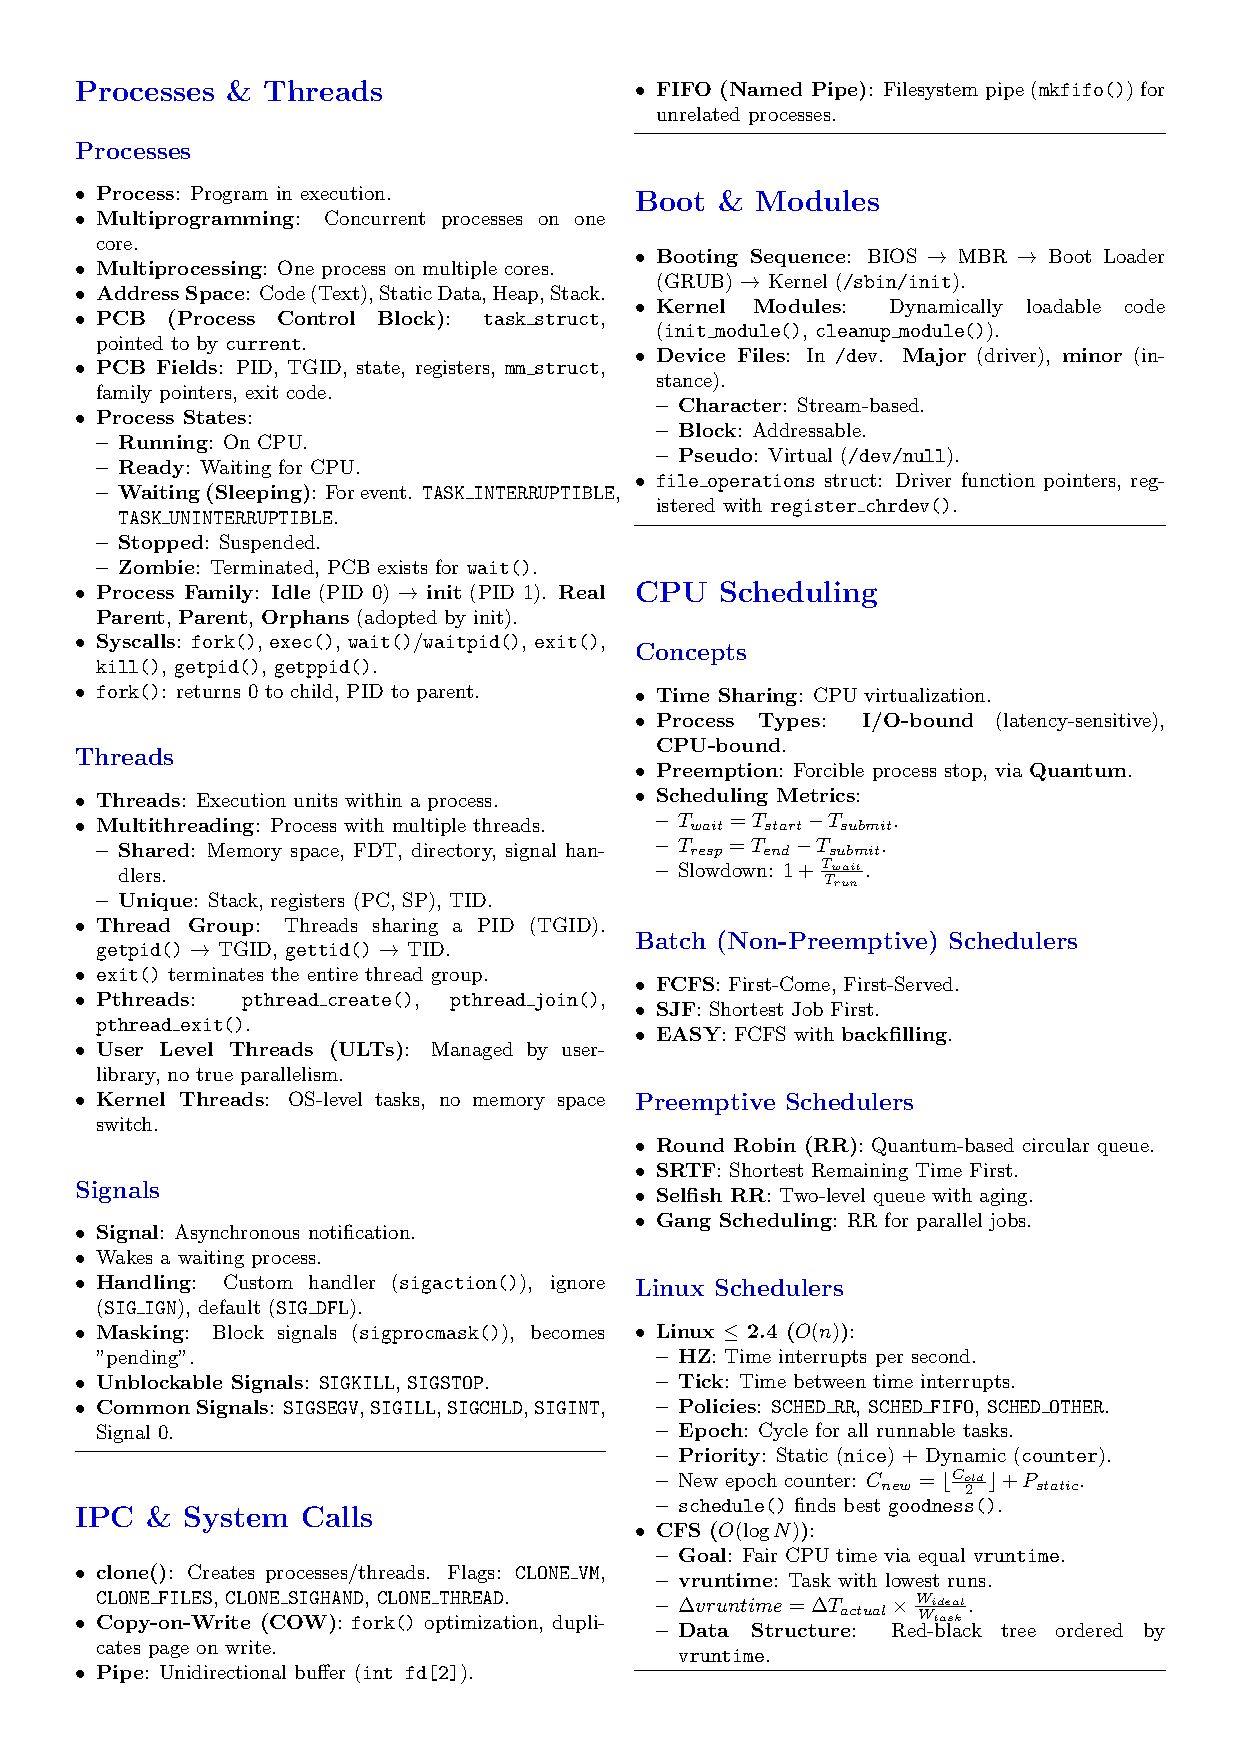
\includepdf[pages=-]{../Cheat Sheet/cheat sheet.pdf}




\end{document}